\documentclass{beamer}
\usetheme[subsectionpage=progressbar, background=white]{metropolis}
\usepackage[utf8]{inputenc}
\usepackage{graphicx,color}
\usepackage{amsfonts}
\usepackage{amsmath}
\usepackage{amssymb}
\usepackage{verbatim}
\usepackage{fancyhdr}
\usepackage{epigraph}
\usepackage{caption}
\usepackage{psfrag}
\usepackage{afterpage}
\usepackage[backend=biber, style=nature]{biblatex}
\addbibresource{../bibTex/thesis-library.bib}
\useinnertheme{circles}
\graphicspath{{../figures/}}
%\setbeamercovered{transparent}
\newcommand{\Note}[1]{{\bf \color{red}#1}}    %Anotaciones
\newcommand{\esc}{\!\cdot\!}
\newcommand{\llangle}{\left\langle}
\newcommand{\rrangle}{\right\rangle}
\newcommand{\llg}{\left\lgroup}
\newcommand{\rlg}{\right\rgroup}
\newcommand{\bra}{\llbracket}
\newcommand{\ket}{\rrbracket}
\newcommand{\cc}{\!\parallel\!}
\newcommand{\GK}[2]{\langle#1 \cc #2\rangle}
\newcommand{\GKrest}[2]{\langle#1 \cc #2\rangle^0}




\title{Nanoscale hydrodynamics near solids}
\date{June 2019}
\author{Diego Duque Zumajo}
\institute{Departamento Física Fundamental \\Universidad Nacional de Educación a Distancia}

% logo of my university
\titlegraphic{%
\begin{picture}(0,0)
\put(308,-119){\makebox(0,0)[rt]{
\includegraphics[width=1.5cm]{logo}}}
\end{picture}}

\begin{document}
\maketitle

\begin{frame}{Motivation}
\end{frame}

\end{document}
%\begin{frame}
%\frametitle{Agenda}
%\tableofcontents
%\end{frame}

%\section{Introduction}
%\begin{frame}{Roadmap}
%  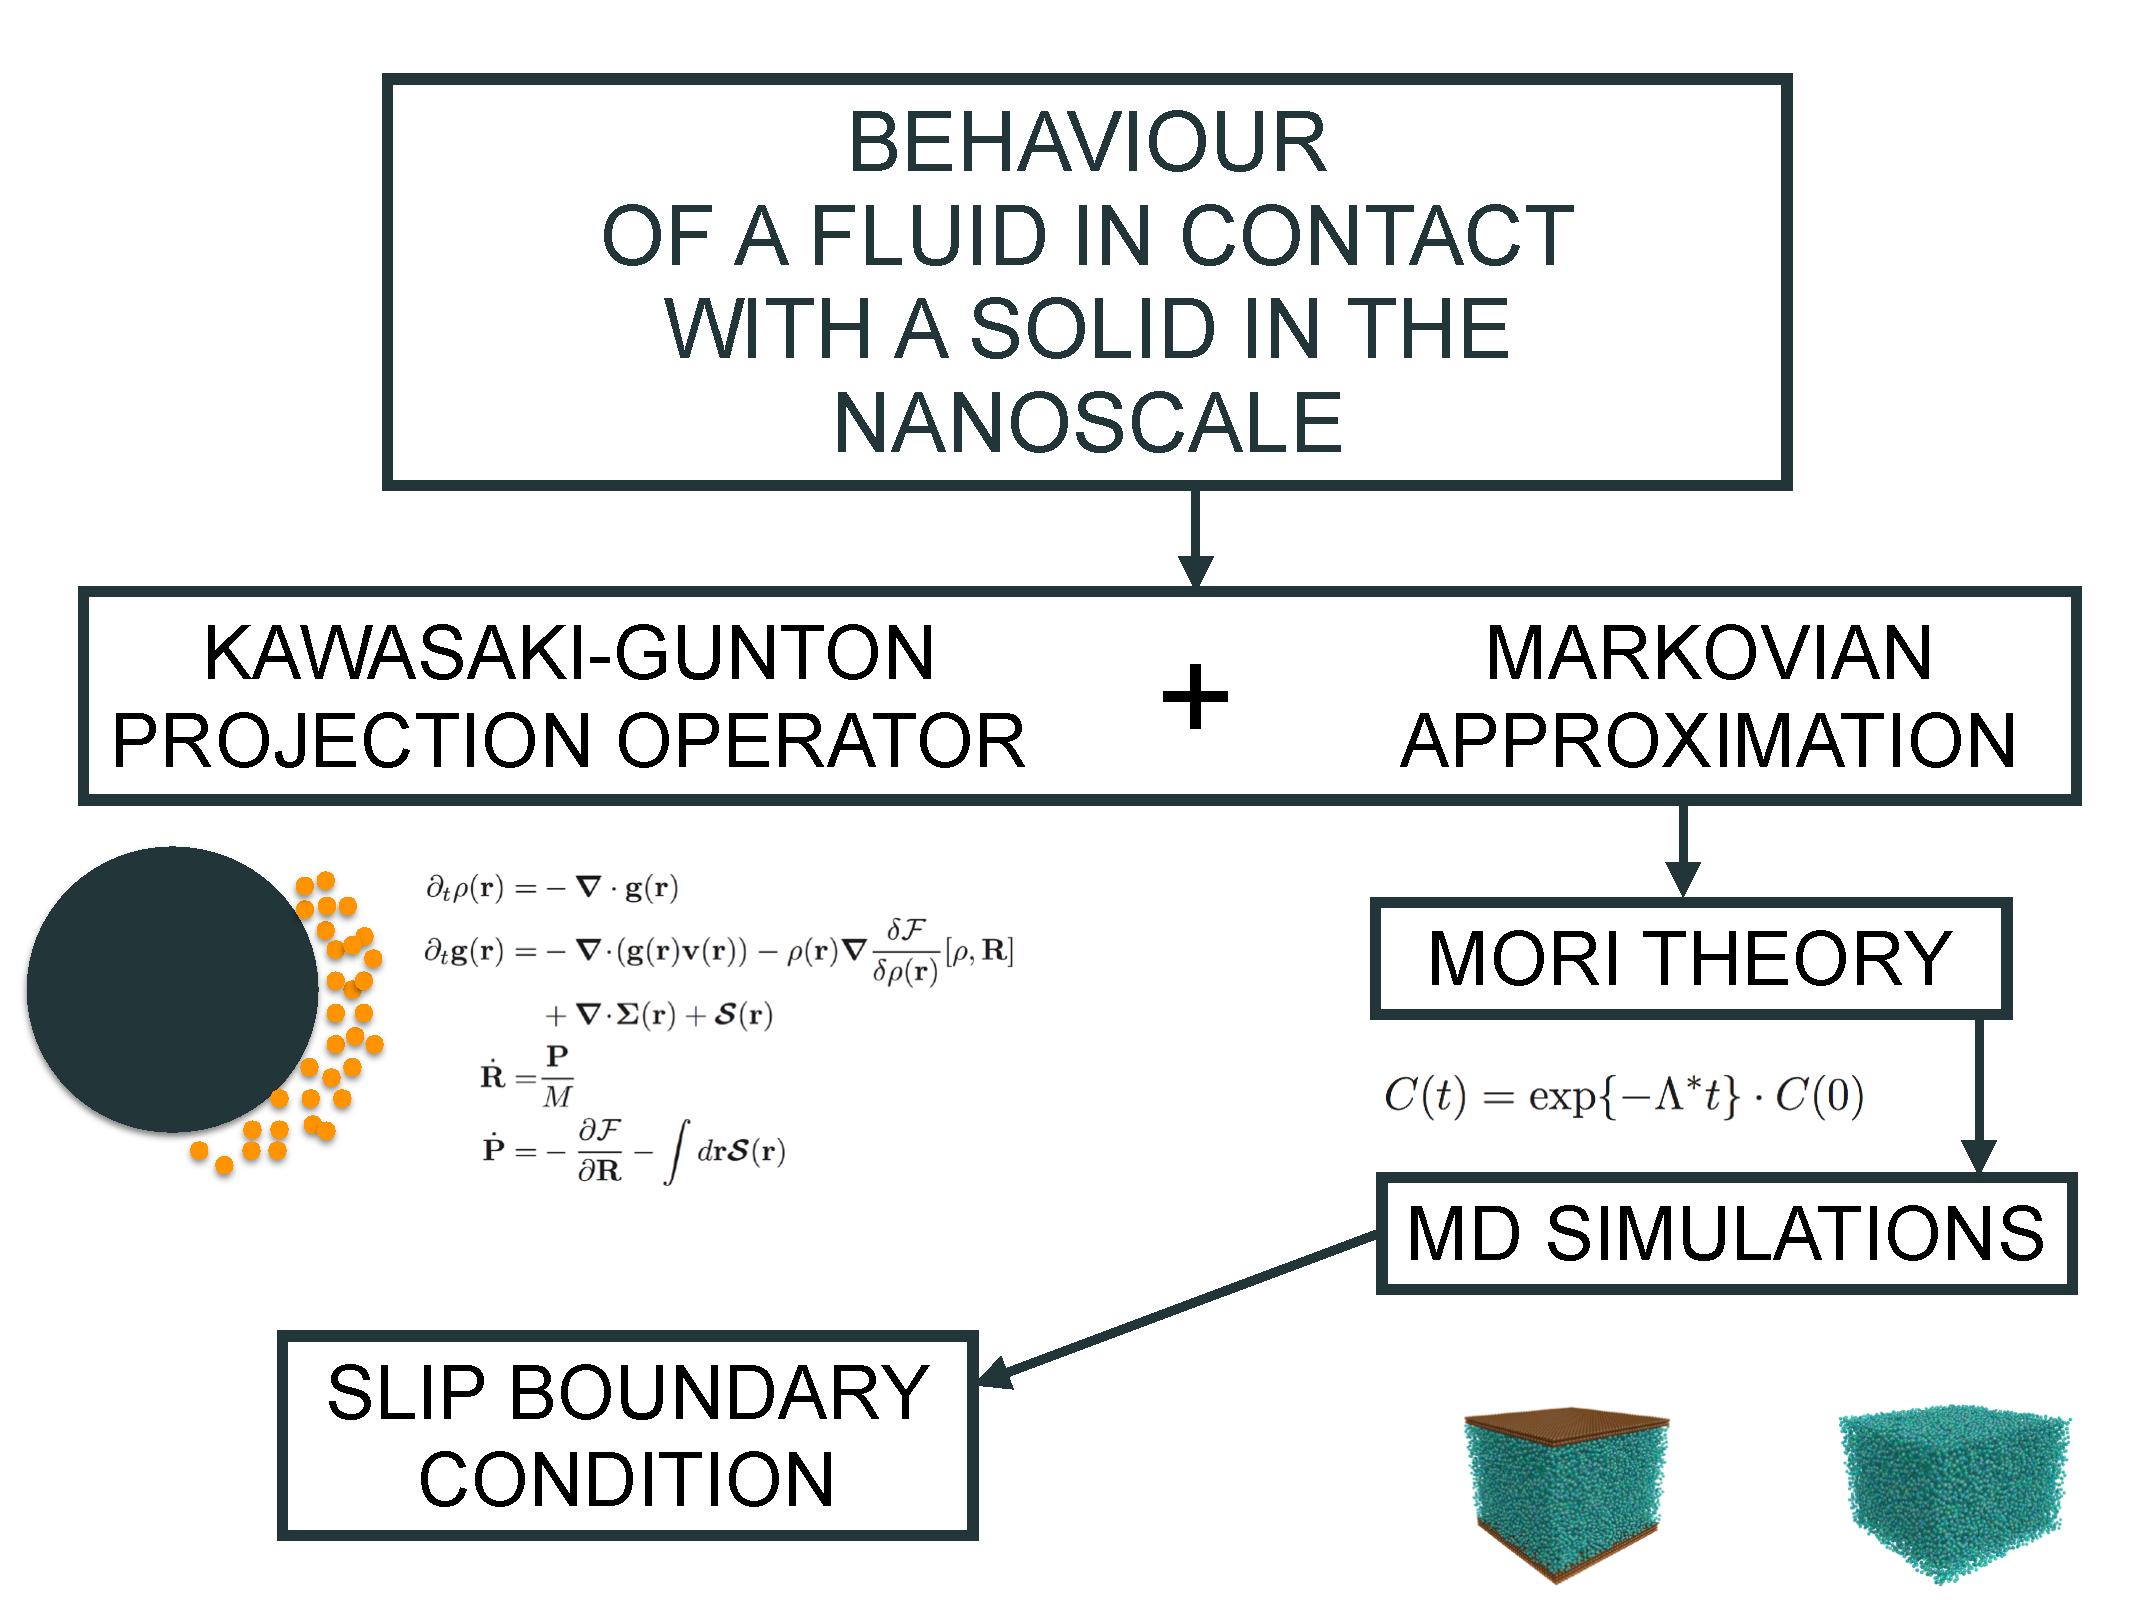
\includegraphics[width=\linewidth]{scheme-thesis}
%\end{frame}
%
%\begin{frame}{Derivation of the slip boundary condition}
%\begin{itemize}
%\item Through the  measurement of the correlation of
%the  transverse  momentum  and  comparison  with  the  predictions  of
%continuum  (local) hydrodynamics  \cite{Bocquet1993,Chen2015}.
%\item Through
%linear  response theory  relating  the  force on  the  walls with  the
%velocity   of  the   fluid   \cite{Bocquet1993,Petravic2007}.
%\item By formulating  linear,  in  general  non-Markovian,  conections  between
%friction forces and velocities \cite{Hansen2011}, where the meaning of
%this quantities is often understood implicitly.
%\end{itemize}
%\end{frame}
%
%\begin{frame}{The slip problem from first principles}
%  \begin{itemize}
%\item Hydrodynamic equations from the microscopic dynamics of a fluid \cite{Piccirelli1968}.
%\item Molecular Dynamics simulations in order to measure the transport coefficients that appear in the hydrodynamic equations in order to validate the theory.
%\item The slip boundary condition is measured from a microscopic definition of the slip lenght and the position of the atomic wall. 
%\end{itemize}
%\end{frame}
%
%\section{Nonequilibrium Statistical Mechanics}
%\begin{frame}{The Theory of Coarse-Graining (ToCG)}
%\begin{itemize}
%\item The ToCG consists on eliminate the ``useless'' information about a system. 
%\item We select the relevant variables or Coarse grained (CG) variables.
%%Selected variables with timescales much larger than the typical molecular scales. 
%\item Levels of description depending on the amount of information which one retains macroscopically.
%  \begin{itemize}
%    \item Macroscopic level.
%    \item Microscopic level.
%    \item Mesoscopic level.
%    \end{itemize}
%\end{itemize}
%\end{frame}
%
%\begin{frame}{The entropy}
%  \begin{itemize}
%    \item The average of the CG variables $\hat{A}$
%  \begin{align}
%    a = {\rm Tr}[{\hat{A}}\rho]
%    \nonumber
%\end{align}
%  \item 
%The trace symbol is given by
%\begin{align}
%  {\rm Tr}\left[\cdots\right]&=\sum_{N=0}^\infty \frac{1}{N!h^{3N}}
%\int dz'\cdots
%\nonumber
%\end{align}
%\item Gibbs-Jaynes entropy functional 
%\begin{align}
% {\cal S}[\rho]&=-{\rm Tr}\left[\rho\ln\frac{\rho}{\rho_0}\right]
%\nonumber
%\end{align}
%%where  $\rho_0=\frac{1}{N!h^{3N}}$
%\item \alert{The relevant ensemble} takes the form
%\begin{equation}
%\overline{\rho}(z) = \frac{1}{Z[\lambda]} \rho_0\exp\{-\lambda\!\cdot\!\hat{A}(z)\}
%\nonumber
%\end{equation}
%with $Z[\lambda]$ the partition function and $\lambda$ the set of conjugate variables.
%\end{itemize}
%\end{frame}
%
%\begin{frame}{The entropy}
%  \begin{itemize}
%    \item The average $a$ with respect to the relevant ensemble is
%   \begin{align}
%  a =\langle \hat{A}\rangle^\lambda ={\rm Tr}[\overline{\rho}\hat{A}]
%     \nonumber
%\end{align}
%\item If we introduce the thermodynamic potential $\Phi[\lambda]=-\ln Z[\lambda]$
%\begin{equation}
%a =\frac{\partial \Phi}{\partial
%\lambda}[\lambda]
%\nonumber
%\end{equation}
%\item One to one connection between $\lambda$ and $a$.
%\item The entropy is the Legendre transform of $\Phi[\lambda]$
%\begin{align}
%  {\cal S}[a] =-\Phi[\lambda[a]]+\lambda[a] a
%\nonumber
%\end{align}
%which is related to the Gibbs-Jaynes entropy functional ${\cal S}[\rho]$ as
%  \begin{align}
%{\cal S}[a]={\cal S}[\overline{\rho}]
%\nonumber
%\end{align}
%\item The averages \alert{$a$ and $\lambda$ are related through the entropy}
%\begin{align}
%  \frac{\partial S}{\partial a}&=\lambda
%\nonumber
%\end{align}
%    \end{itemize}
%\end{frame}
%
%\begin{frame}{The dynamics}
%  \begin{itemize}
%    %\item Set of CG variables $\hat{A}_i(z)$ and their averages $a_i(z)$
%%\begin{align}
%%    a = {\rm Tr}[{\hat{A}}\rho]
%%    \nonumber
%%\end{align}
%    \item The aim is to \alert{derive equations of motion} for the time dependent average $a_i(t)$ of the CG variables $\hat{A}_i(z)$
%      \begin{align}
%        a_i(t)={\rm Tr}\left[\hat{A}_i(z)\rho_t\right]
%        \nonumber
%      \end{align}
%\item $\rho_t$ is the nonequilibrium solution of the Liouville equation
%\begin{align}
%    \rho_t(z) = {\rm exp}\{-i{\cal L}t\}\rho_0(z)
%    \nonumber
%\end{align}
%\item We use two techniques:
%  \begin{enumerate}
%    \item The Kawasaki-Gunton projection operator.
%    \item Mori theory.
%    \end{enumerate}
%  \end{itemize}
%\end{frame}
%
%\begin{frame}{The dynamics. The Kawasaki-Gunton projection operator}
%    For isolated systems with a time-independet Hamiltonian,the averages evolves according to the following equation \cite{Grabert1982}
%      \begin{equation}
%\frac{\partial }{\partial t} a_i(t)
%= v_i(t) + \int_0^t dt' \sum_j K_{ij}(t,t') \lambda_j(t')
%\nonumber
%\end{equation}
%\end{frame}
%
%\begin{frame}{Kawasaki-Gunton projection operator. The reversible term}
%\begin{itemize}
%  \item The reversible term is given by
%\begin{equation}
%  v_i(t) = {\rm Tr}[\overline{\rho}_t  i{\cal L} \hat{A}_i]
%  \nonumber
%\end{equation}
%where $i{\cal L}$ is the Liouville operator and $\overline{\rho}_t$ is the \alert{relevant ensemble} which maximizes the Gibbs-Jaynes entropy functional
%\begin{align}
% {\cal S}[\rho]&=-{\rm Tr}\left[\rho\ln\frac{\rho}{\rho_0}\right]
%\nonumber
%\label{entropy}
%\end{align}
%
%\item The form of $\overline{\rho}_t$ is
%\begin{equation}
%\overline{\rho}(z) = \frac{1}{Z[\lambda]} \rho_0\exp\{-\lambda\!\cdot\!\hat{A}(z)\}
%\nonumber
%\end{equation}
%where $Z[\lambda]$ is the partition function and $\rho_0=\frac{1}{N!h^{3N}}$,   with  $h$  being   the  Planck's constant.
%\end{itemize}
%\end{frame}
%
%\begin{frame}{Kawsaki-Gunton projection operator. The irreversible term}
%\begin{itemize}
%    \item The irreversible
%      term involves the \alert{memory kernel}
%\begin{equation}
%K_{ij}(t,t') =
%{\rm Tr}\left[\overline{\rho}_{t'} 
%  \left({\cal Q}_{t'} i{\cal L}\hat{A}_j\right) G_{t't}
%\left({\cal Q}_{t } i{\cal L}\hat{A}_i\right)\right]
%\nonumber
%\label{ker}
%\end{equation}
%where   the  Kawasaki-Gunton   projection  operator   ${\cal  Q}_{t'}$
%applied  to an  arbitrary  function
%$\hat{F}(z)$ is
%\begin{align}
%  {\cal Q}_{t'}\hat{F}(z) &= \hat{F}(z)- {\rm Tr}[\overline{\rho}_{t'} \hat{F}]
%-\sum_i(\hat{A}_i(z)-a_i(t'))\frac{\partial }{\partial a_i(t')}
%{\rm Tr}[\overline{\rho}_{t'} \hat{F}]
%\label{Q}
%\nonumber
%\end{align}
%
%\item The time ordered projected propagator $G_{t't}$ is given by
%\begin{align}
%  G_{t't}&=1
%+\sum_{n=1}^\infty \int_{t'}^tdt_1\cdots\int_{t'}^{t_{n-1}}dt_n
%i{\cal L}{\cal Q}_{t_n}\cdots  i{\cal L}{\cal Q}_{t_1}
%\nonumber\\
%&\equiv T_+\exp\left\{\int_{t'}^t dt''  i{\cal L}{\cal Q}_{t''}\right\}
%\nonumber
%\end{align}
%where $T_+$ ensures that the operators are ordered from left to right as time increases.
%\end{itemize}
%  
%\end{frame}
%
%\begin{frame}{Kawasaki-Gunton projection operator. Markovian equation}
%  \begin{itemize}
%     \item Clear separation of timescales between the evolution of the averages and the decay of the memory kernel 
%\begin{equation}
%  \frac{\partial}{\partial t}a_i(t) = v_i(t) + \sum_j D_{ij}(t) \lambda_j(t)
%\nonumber
%\end{equation}
%\item The  dissipative matrix  is  given  by  the Green-Kubo  formula
%\begin{equation}
%D_{ij}(t)=\int_0^{\Delta t} dt'\left\langle 
%{\cal Q}_t i{\cal L}\hat{A}_j\exp\{i{\cal L}t'\}{\cal Q}_t i{\cal L}\hat{A}_i
%\right\rangle^{\lambda(t)}
%\label{dij}
%\nonumber
%\end{equation}
%\item $\left\langle\cdots\right\rangle$ denotes an equilibrium average.
%\end{itemize}
%\end{frame}
%
%\begin{frame}{The dynamics. Mori theory}
%    The \alert{Mori's exact Generalized Langevin equation} \cite{Mori1965} is
%\begin{align}
%  \frac{d}{dt}\hat{A}(t)= & -L\esc C^{-1}(0)\esc \hat{A} (t) 
%  -\int_0^tdt'\Gamma(t-t')\esc  C^{-1}(0)\esc \hat{A} (t') +F^+(t)
%\nonumber
%\end{align}
%where the following matrices have been introduced
%\begin{align}
%  L&=\langle \hat{A}i{\cal L}\hat{A}^T\rangle \nonumber \\
%  C(0)&=\langle \hat{A}\hat{A}^T\rangle \nonumber \\
%\Gamma(t)&=\langle F^+(t)F^{+T}(0)\rangle
%\nonumber
%\end{align}
%\end{frame}
%
%\begin{frame}{Mori theory. Projected forces and projection operator}
%  \begin{itemize}
%\item The projected forces are given by
%\begin{align}
%F^+(t)&= \exp\{{\cal Q}i{\cal L}t\} {\cal Q}i{\cal L}\hat{A}  
%\nonumber
%\end{align}
%\item $F^+(t)$ have zero mean and are uncorrelted from preivous values of the CG variables
%\begin{align}
%\langle  F^+  (t)\rangle&=0  
%\nonumber\\
%\langle \hat{A} F^+ (t)\rangle&=0 \quad\quad t\ge 0
%\nonumber
%\end{align}
%\item The projection operator ${\cal Q}$ is defined as ${\cal Q}=1-{\cal P}$
%  where  ${\cal P}$  is \alert{Mori's  projector} whose  effect on  an arbitrary
%phase function $\hat{F}(z)$ is
%\begin{align}
%  {\cal P}\hat{F}(z) = \langle \hat{F}\rangle+ \langle \hat{F}\hat{A}^T \rangle\esc  C^{-1}(0)\esc  \hat{A}(z)
%\nonumber
%\end{align}
%\end{itemize}
%\end{frame}
%\begin{frame}{Mori theory. Correlations and averages}
%  \begin{itemize}
%    \item The equilibrium time  correlation matrix of the CG variables is 
%\begin{align}
%  C(t)&=  \llangle \hat{A}(t)\hat{A}^T\rrangle
%\nonumber
%\end{align}
%\item \alert{Mori's equation for correlations}
%\begin{align}
%  \frac{d}{dt}C(t)&=-L\esc C^{-1}(0)\esc C(t)
%-\int_0^tdt' \Gamma(t-t')\esc C^{-1}(0)\esc  C(t')
%\nonumber
%\end{align}
%
%\item The time-dependent average of the CG variables is defined as
%\begin{align}
%  a(t)&=\int dz \rho_0(z) \exp\{i{\cal L}t\}\hat{A}(z)
%  \nonumber
%\end{align}
%\item \alert{Mori's equation for averages}
%\begin{align}
%  \frac{d}{dt}a(t) = -L\esc C^{-1}(0)\esc a(t)
%-\int_0^tdt' \Gamma(t-t')\esc  C^{-1}(0)\esc a(t')
%\label{exactAve}
%\nonumber
%\end{align}
%\end{itemize}
%\end{frame}
%
%\begin{frame}{Mori theory. Markovian aproximation}
%  \begin{itemize}
%    \item The linear integro-differential term can be approximated by a memory-less term
%      \begin{align}
%  \frac{d}{dt}C(t)&=-L\esc C^{-1}(0)\esc C(t)
%  -\underbrace{\int_0^tdt' \Gamma(t-t')\esc C^{-1}(0)\esc  C(t')}_{M^* C^{-1}(0)C(t)}
%\nonumber
%\end{align}
%\item Evolution equation for the correlations
%\begin{align}
%  \frac{d}{dt}C(t)&=-(L+M^*)C^{-1}(0)C(t) 
%  \nonumber \\
%  &= \Lambda^*\esc  C(t)
%\nonumber
%\end{align}
%\item The \alert{relaxation matrix} $\Lambda^*$ is defined as
%\begin{align}
%\Lambda^*\equiv(L+M^*)\esc C^{-1}(0)  
%\nonumber
%\end{align}
%\end{itemize}
%\end{frame}
%
%\begin{frame}{Mori theory. Markovian aproximation}
%  \begin{itemize}
%    \item  The only possibility for a correlation is to \alert{decay in an exponential matrix way} 
%\begin{align}
%  C(t)=\exp\{-\Lambda^* t\}\esc C(0)
%\nonumber
%\end{align}
%\item At short times 
%\begin{align}
%    \frac{d}{dt}C(0)&=-L
%  \nonumber
%\end{align}
%which is only possible if $M^*=0$.
%\item The correlations  will decay  in an
%  exponential (Markovian)  way only  after the  time $\tau$  beyond which
%memory is lost. 
%\begin{align}
%  C(t)=\exp\{-\Lambda^* (t-\tau)\}\esc C(\tau)
%\nonumber
%\end{align}
%\item Onsager's regression hypothesis
%\begin{align}
%  a(t)=\exp\{-\Lambda^* (t-\tau)\}\esc a(\tau)
%\nonumber
%\end{align}
%\end{itemize}
%\end{frame}
%
%\begin{frame}{Summary}
%\begin{itemize}
%\item Kawasaki-Gunton equation with Markovian approximation
%\begin{equation}
%\frac{\partial}{\partial t}a_i(t) = v_i(t) + \sum_j D_{ij}(t) \lambda_j(t)
%\nonumber
%\end{equation}
%\item Mori equation with Markovian approximation
%\begin{align}
%\frac{d}{dt}C(t)=\Lambda^*C(t)
%\nonumber
%\end{align}
%\item Exponential decay of the matrix of correlations after a time $\tau$.
%\begin{align}
%C(t)=\exp\{-\Lambda^* (t-\tau)\}\esc C(\tau)
%\nonumber
%\end{align}
%\end{itemize}
%\end{frame}
%
%\section{Hydrodynamics theory for liquids near solids}
%\begin{frame}{The system}
%  \begin{itemize}
%    \item Liquid system of $N$ particles interacting with a solid sphere of $N'$ particles.
%    \item The system is described  by the set of all  positions  ${\bf  q}_i$  and  momenta  ${\bf  p}_i=m_i{\bf  v}_i$
%($i=1,\cdots,N$) of the liquid atoms plus the positions ${\bf q}_{i'}$
%and  momenta ${\bf  p}_{i'}=m_{i'}{\bf v}_{i'}$  ($i'=1,\cdots,N'$) of
%the atoms  of the solid  sphere. 
%\item The microstate $z={q,p,q',p'}$. 
%    \item The microstate of the system evolves according to Hamilton's equations 
%\begin{align}
%H(z) = \sum^N_i \frac{p_i^2}{2m_i} + \sum^{N'}_{i'} \frac{p_{i'}^2}{2m_{i'}}
%+ U(z)
%\nonumber
%\end{align}
%\end{itemize}
%\end{frame}
%
%\begin{frame}{The CG variables}
%  \begin{itemize}
%    \item The CG variables
%\begin{align}
%  \hat{\rho}_{\bf r}(z) &=\sum^{N}_im\delta({\bf r}-{\bf q}_i)
%&&\hat{\bf R}(z)=\frac{1}{N'}\sum_{i'}^{N'}{\bf q}_{i'}
%\nonumber\\
%  \hat{\bf g}_{\bf r}(z) &=\sum^{N}_i{\bf p}_i\delta({\bf r}-{\bf q}_i)
%&&\hat{\bf P}(z)=\sum_{i'}^{N'}{\bf p}_{i'}
%\nonumber
%\end{align}
%\item The derivatives of the CG variables
%\begin{align}
%  i{\cal L} \hat{\rho}_{\bf r}(z) &= -\boldsymbol{\nabla}\esc\hat{\bf g}_{\bf r}(z)
%  && i{\cal L}\hat{\bf R}(z) =\frac{\hat{\bf P}(z)}{M}
%\nonumber\\
%i{\cal L}\hat{\bf g}_{\bf r}(z)
%    &=-\boldsymbol{\nabla}\cdot \hat{\boldsymbol{\sigma}}_{\bf r}(z)+\hat{{\bf F}}^{\rm s\to l}_{\bf r}(z) 
%  &&i{\cal L}\hat{\bf P}(z) =-\int  d{\bf r} \hat{\bf F}^{\rm s\to l}_{\bf r}(z)
%   \nonumber
%\end{align}
%    \end{itemize}
%\end{frame}
%
%\begin{frame}{The relevant enesemble}
%  \begin{itemize}
%    \item The ensemble which maximizes the Gibbs-Jaynes entropy functional is
%\begin{align}
%  \overline{\rho}(z)&=\frac{1}{\Xi[\lambda]}\rho_0\exp\left\{-\beta H(z)\right\}
%\nonumber\\
%&\times
%\exp\left\{-\beta\int d{\bf r}\left(\lambda_\rho({\bf r})\cdot\hat{\rho}_{\bf
%    r}(z)+\boldsymbol{\lambda}_g{({\bf r})\cdot}\hat{\bf g}_{\bf r}(z)\right)\right\}
%\nonumber\\
%&\times
%\exp\left\{-\beta \boldsymbol{\lambda}_{R}\esc\hat{\bf R}(z)
%-\beta \boldsymbol{\lambda}_{P}\esc\hat{\bf P}(z)\right\}
%\nonumber
%\end{align}
%\item The $\lambda$-dependent partition function is
%\begin{align}
%  \Xi[\lambda]
%  &\equiv
% \sum_{N=0}^\infty \frac{1}{N!h^{3N}}
%\int dqdp dq'dp'
%\nonumber\\
%&\times\exp\left\{-\beta H-\beta \sum_{i=1}^Nm \lambda_\rho({\bf
%    q}_i)-\beta \sum_{i=1}^N{\bf p}_i\esc\boldsymbol{\lambda}_g({\bf q}_i)\right\}
%\nonumber\\
%&\times\exp\left\{-\beta \boldsymbol{\lambda}_{R}\esc\hat{\bf R}(z)
%-\beta \boldsymbol{\lambda}_{P}\esc\hat{\bf P}(z)\right\}
%\nonumber
%\end{align}
%\end{itemize}
%\end{frame}
%
%\begin{frame}{The grand potential}
%  \begin{itemize}
%\item The $\lambda$-dependent grand-canonical potential is given by
%\begin{eqnarray}
%  \Phi [\lambda]\equiv-k_BT \ln\Xi [\lambda]
%\nonumber
%\end{eqnarray}
%
%\item There is a one to one connection between the averages of the CG variables and the conjugates ones
%\begin{align}
%  \rho({\bf r}) &=\frac{\delta \Phi [\lambda]}{\delta \lambda_\rho({\bf r}) }
%&&{\bf R} =\frac{\partial \Phi [\lambda]}{\partial \boldsymbol{\lambda}_R }
%\nonumber\\
%  {\bf g}({\bf r}) &=\frac{\delta \Phi [\lambda]}{\delta \boldsymbol{\lambda}_g({\bf r}) }
%&&{\bf P} =\frac{\partial \Phi [\lambda]}{\partial \boldsymbol{\lambda}_P }
%\nonumber
%\end{align}
%\end{itemize}
%\end{frame}
%
%\begin{frame}{The hydrodynamic functional}
%  \begin{itemize}
%\item The hydrodynamic functional 
%\begin{align}
%    {\cal H}[\rho,{\bf g},{\bf R},{\bf P}] =&
%\Phi [\lambda_\rho,\boldsymbol{\lambda}_g,\boldsymbol{\lambda}_R,\boldsymbol{\lambda}_P]
%\nonumber\\
%    & -
%\int d{\bf r}\rho({\bf r})\lambda_\rho({\bf r})
%-
%\int d{\bf r}{\bf g}({\bf r})\cdot\boldsymbol{\lambda}_g({\bf r})
%\nonumber\\
%    &    -\boldsymbol{\lambda}_R\cdot{\bf R}-\boldsymbol{\lambda}_P\cdot{\bf P}
%\nonumber
%\end{align}
%\item The hydrodynamic functional is minus the entropy 
%\begin{align}
%  \lambda_\rho({\bf r}) &=-\frac{\delta {\cal H}}{\delta \rho({\bf r}) }
%&&  \boldsymbol{\lambda}_R =-\frac{\partial {\cal H}}{\partial {\bf R} }
%\nonumber\\
%  \boldsymbol{\lambda}_g({\bf r}) &=-\frac{\delta {\cal H}}{\delta {\bf g}({\bf r}) }
%&&  \boldsymbol{\lambda}_P =-\frac{\partial {\cal H}}{\partial{\bf P} }
%\nonumber
%\end{align}
%\end{itemize}
%\end{frame}
%
%\begin{frame}{The grand potential of a fluid in the presence of a sphere}
%  \begin{itemize}
%    \item 
%  We may express the gran potential $\Phi [\lambda]$ as a sum of two contributions
%\begin{align}
%\Phi [\lambda]&=  \Phi^{\rm pos}[\mu,\boldsymbol{\lambda}_R]
%-\frac{M'}{2} {\boldsymbol{\lambda}_P}^2,
%\nonumber
%\end{align}
%where we have defined the following grand potential
%\begin{align}
%\Phi^{\rm pos}[\mu,\boldsymbol{\lambda}_R]
%&\equiv-k_BT\ln
% \sum_{N=0}^\infty \frac{1}{N!}
%\int \frac{dq}{\Lambda^{3N}}\frac{dq'}{\Lambda^{3N'}}\nonumber\\
%&\times
%\exp\left\{-\beta  \left(U-\sum_{i=1}^N m\cdot\mu({\bf
%    q}_i)+ \boldsymbol{\lambda}_R\cdot\hat{\bf R}\right)\right\}
%\nonumber
%\end{align}
%\item We have introduced the thermal wavelength  and the chemical potential
%\begin{align}
%  \Lambda=\left(\frac{h^2\beta}{2\pi m}\right)^{\frac{1}{2}}, &&
%  \mu({\bf r})&\equiv\frac{1}{2}\lambda_g^2({\bf r})-\lambda_\rho({\bf r})
%\nonumber
%\end{align}
%\end{itemize}
%\end{frame}
%
%\begin{frame}{The free energy}
%  \begin{itemize}
%    \item The Legendre transform of the grand potential for a simple fluid gives the classic free energy density functional.
%    \item The free energy functional ${\cal  F}[\rho,{\bf R}]$ of a structured fluid in the presence of a solid sphere is
%\begin{align}
%  {\cal F}[\rho,{\bf R}]&\equiv  \Phi^{\rm pos}[\mu,\boldsymbol{\lambda}_R]
%+
%\int d{\bf r}\rho({\bf r})\mu({\bf r})-\boldsymbol{\lambda}_R\cdot{\bf R},
%\nonumber
%\end{align}
%\item Finally, the hydrodynamic funcional ${\cal H}$ takes the form
%\begin{align}
%  \frac{\delta {\cal H}}{\delta\rho({\bf r})}[\rho,{\bf g},{\bf R},{\bf P}] &=    
%\frac{{\bf v}^2({\bf r})}{2}+  \frac{\delta {\cal F}}{\delta\rho({\bf r})}[\rho,{\bf R}]
%\nonumber
%\end{align}
%\end{itemize}
%\end{frame}
%
%%\begin{frame}{The transport equations}
%%  \begin{itemize}
%%    \item
%%Kawasaki-Gunton equation 
%%\begin{equation}
%%  \frac{\partial}{\partial t}a_i(t) = v_i(t) + \sum_j D_{ij}(t) \lambda_j(t)
%%\nonumber
%%\end{equation}
%%\item 
%%\end{itemize}
%%\end{frame}
%
%\begin{frame}{The transport equations. Reversible term}
%  \begin{itemize}
%    \item The reversible term has the form
%\begin{equation}
%  v_i(t) = {\rm Tr}[\overline{\rho}_t  i{\cal L} \hat{A}_i]
%  \nonumber
%\end{equation}
%\item Reversible equations for the CG variables
%\begin{align}
%\left.  \partial_t\rho({\bf r})\right|_{\rm rev}&=-\boldsymbol{\nabla}\cdot{\bf g}({\bf r})
%\nonumber\\
%\left.  \partial_t{\bf g}({\bf r})\right|_{\rm rev}&=-\boldsymbol{\nabla}\cdot\left({\bf g}({\bf r}){\bf v}({\bf r})\right)
%-\rho({\bf r})\boldsymbol{\nabla} \frac{\delta {\cal F}}{\delta\rho({\bf r})}[\rho,{\bf R}]
%\nonumber\\
%\partial_t\left. {\bf R}\right|_{\rm rev}&=\frac{\bf P}{M}
%\nonumber\\
%\partial_t\left.{\bf P}\right|_{\rm rev}&=-\frac{\partial {\cal F}}{\partial {\bf R}}[\rho,{\bf R}]
%\nonumber
%\end{align}
%  \item No approximations.
%  \item They conserve the hydrodynamic functional ${\cal H}$.
%\end{itemize}
%\end{frame}
%
%\begin{frame}{The transport equations. Irreversible term}
%  \begin{itemize}
%    \item The irreversible term has the form 
%        $\sum_{j}D_{ij}(t)\lambda_{j}(t)$
%    \item With
%$D_{ij}(t)=\int_0^{\Delta t} dt'\left\langle 
%{\cal Q}_t i{\cal L}\hat{A}_j\exp\{i{\cal L}t'\}{\cal Q}_t i{\cal L}\hat{A}_i
%\right\rangle^{\lambda(t)}$
%\item Large simplificatin of the friction matrix because 
%${\cal Q} i{\cal L}\hat{\rho}_{\bf r}=0$
%and ${\cal Q}  i{\cal L}\hat{{\bf R}}_{\mu}=0$
%\item Irreversible equations for the CG variables
%\begin{align}
%\left.  \partial_t{\bf g}^\alpha({\bf r})\right|_{\rm irr}&= \boldsymbol{\nabla}_{\bf r}^{\beta}\boldsymbol{\Sigma}^{\alpha\beta}({\bf r}) +\boldsymbol{{\cal S}}^\alpha({\bf r}) 
%\nonumber\\
%\left.\frac{d}{dt}{\bf P}^\alpha(t)\right|_{\rm irr}&=-\int d{\bf r}'   \boldsymbol{{\cal S}}^\alpha({\bf r}'),
%\nonumber
%\end{align}
%%\item 
%%\begin{align}
%%  \partial_t{\bf g}({\bf r})&=-\int d{\bf r}'M^{gg}_{{\bf r}{\bf r}'}
%%{\bf v}({\bf r}')-M^{gP}_{\bf r}{\bf V}
%%\nonumber\\
%%\frac{d}{dt}{\bf P}(t)&=-\int d{\bf r}' M^{Pg}_{{\bf r}'}{\bf v}({\bf r}')-M^{PP}{\bf V}
%%\nonumber
%%\end{align}
%\end{itemize}
%\end{frame}
%
%\begin{frame}{The transport equations. Irreversible term}
%  \begin{itemize}
%    \item The fluid \alert{stress tensor}
%  \begin{align}
%  \boldsymbol{\Sigma}^{\alpha\beta}({\bf r})&=
%\int d{\bf r}'
%\boldsymbol{\eta}^{\alpha\beta\alpha'\beta'}_{{\bf r}{\bf r}'}
%\boldsymbol{\nabla}_{{\bf r}'}^{\beta'}{\bf v}^{\alpha'}({\bf r}')
%\nonumber
%\end{align}
%\item The \alert{irreversible surface force density} on the fluid
%\begin{align}
%  \boldsymbol{{\cal S}}^\alpha({\bf r})=&
%-\int d{\bf r}'{\bf G}^{\alpha\alpha'\beta'}_{{\bf r}{\bf r}'}
%\boldsymbol{\nabla}_{{\bf r}'}^{\beta'} {\bf v}^{\alpha'}({\bf r}')
%+\boldsymbol{\nabla}_{{\bf r}}^{\beta}\int d{\bf r}'{\bf H}^{\alpha\beta\alpha'}_{{\bf r}{\bf r}'}
%( {\bf v}^{\alpha'}({\bf r}')-{\bf V}^{\alpha'})
%\nonumber\\
%&-\int d{\bf r}'
%\boldsymbol{\gamma}^{\alpha\alpha'}_{{\bf r}{\bf r}'}( {\bf v}^{\alpha'}({\bf r}')
%-{\bf V}^{\alpha'})
%\nonumber
%\end{align}
%\end{itemize}
%\end{frame}
%
%%\begin{frame}
%%  \begin{itemize}
%%\item 
%%\begin{align}
%%  M^{gg}_{{\bf r}{\bf r}'}&=\frac{1}{k_BT}\int_0^{\Delta t} dt\langle 
%%  {\cal Q}  i{\cal L}\hat{\bf g}_{{\bf r}}(t){\cal Q}  i{\cal L}\hat{\bf g}_{{\bf r}'}\rangle^\lambda
%%\nonumber\\
%%  M^{gP}_{{\bf r}}&=\frac{1}{k_BT}\int_0^{\Delta t} dt\langle 
%%{\cal Q}  i{\cal L}\hat{\bf g}_{\bf r}(t){\cal Q}  i{\cal L}\hat{\bf P}\rangle^\lambda
%%\nonumber\\
%%  M^{Pg}_{{\bf r}'}&=\frac{1}{k_BT}\int_0^{\Delta t} dt\langle 
%%{\cal Q}  i{\cal L}\hat{\bf P}(t){\cal Q}  i{\cal L}\hat{\bf g}_{{\bf r}'}\rangle^\lambda
%%\nonumber\\
%%  M^{PP}&=\frac{1}{k_BT}\int_0^{\Delta t} dt\langle 
%%{\cal Q}  i{\cal L}\hat{\bf P}(t){\cal Q}  i{\cal L}\hat{\bf P}\rangle^\lambda
%%\nonumber\\
%%\label{Ms}
%%\end{align}
%%\end{itemize}
%%\end{frame}
%\begin{frame}{Irreversible term. Nonlocal transport coefficients}
%\begin{align}
%  \boldsymbol{\eta}_{{\bf  r}{\bf r}'} &\equiv
%\frac{1}{k_BT}\int_0^{\Delta t} dt'\langle 
%{\cal Q}_t\hat{\boldsymbol{\sigma}}_{{\bf r}}(t')
%{\cal Q}_t\hat{\boldsymbol{\sigma}}_{{\bf r}'}\rangle^{\lambda(t)}
%\nonumber\\
%{\bf H}_{{\bf r}{\bf r}'}&\equiv\frac{1}{k_BT}\int_0^{\Delta t} dt'
%\langle {\cal Q}_t\hat{\boldsymbol{\sigma}}_{{\bf r}}(t')
%{\cal Q}_t\hat{\bf F}^{\rm s\to l}_{{\bf r}'}\rangle^{\lambda(t)}
%\nonumber\\
%{\bf G}_{{\bf r}{\bf r}'}&\equiv\frac{1}{k_BT}\int_0^{\Delta t} dt'
%\langle {\cal Q}_t\hat{\bf F}^{\rm s\to l}_{{\bf r}}(t')
%{\cal Q}_t\hat{\boldsymbol{\sigma}}_{{\bf r}'}\rangle^{\lambda(t)}
%\nonumber\\
%\boldsymbol{\gamma}_{{\bf  r}{\bf r}'}&\equiv\frac{1}{k_BT}\int_0^{\Delta t} dt'
%\langle 
%{\cal Q}_t\hat{\bf F}^{\rm s\to l}_{{\bf r}}(t')
%{\cal Q}_t\hat{\bf F}^{\rm s\to l}_{{\bf r}'}\rangle^{\lambda(t)}
%\nonumber
%\end{align}
%\end{frame}
%
%\begin{frame}{Final equations of nanohydrodynamics}
%\begin{align}
%\partial_t\rho({\bf r})=&-\boldsymbol{\nabla}\cdot{\bf g}({\bf r})
%\nonumber\\
%\partial_t{\bf g}({\bf r})=&-\boldsymbol{\nabla}\esc{\left({\bf g}({\bf r}){\bf v}({\bf r})\right)}
%-\rho({\bf r})\boldsymbol{\nabla}\frac{\delta {\cal F}}{\delta\rho({\bf r})}[\rho,{\bf R}]
%+\boldsymbol{\nabla}\esc\boldsymbol{\Sigma}({\bf r})+\boldsymbol{{\cal S}}({\bf r})
%\nonumber\\
%\dot{\bf R}=&\frac{\bf P}{M}
%\nonumber\\
%\dot{\bf P}=&-\frac{\partial {\cal F}}{\partial {\bf R}}
%-\int d {{\bf r}}\boldsymbol{{\cal S}}({\bf r})
%\nonumber
%\end{align}
%
%\end{frame}
%
%\begin{frame}{From continuum to discrete theory}
%  \begin{itemize}
%    \item The \alert{amount of information} required in the hydrodynamic equations is exceedingly large.
%      \begin{itemize}
%        \item ${\bf \eta}$ 36 independent components. 
%        \item ${\bf H}$ and ${\bf G}$ 21 independent components. 
%        \item ${\bf \gamma}$ 9 independent components. 
%        \end{itemize}
%    \item We need a \alert{simpler theory}. 
%      \begin{itemize}
%        \item Planar walls. 
%        \item Isotropic walls: invariant under translations in the plane of the wall, and under rotations around an axis perpendicular to the walls.
%        \end{itemize}
%    \item \alert{Discrete version} in order to compute MD simulations.
%    \end{itemize}
%\end{frame}
%
%\begin{frame}{The discrete basis function set}
%  \begin{itemize}
%  \item $N_{\rm bin}$ bins with dimensions $L_x$, $L_y$, $\Delta z$ ($L_z/N_{\rm bin}$). 
%      \begin{center}
%    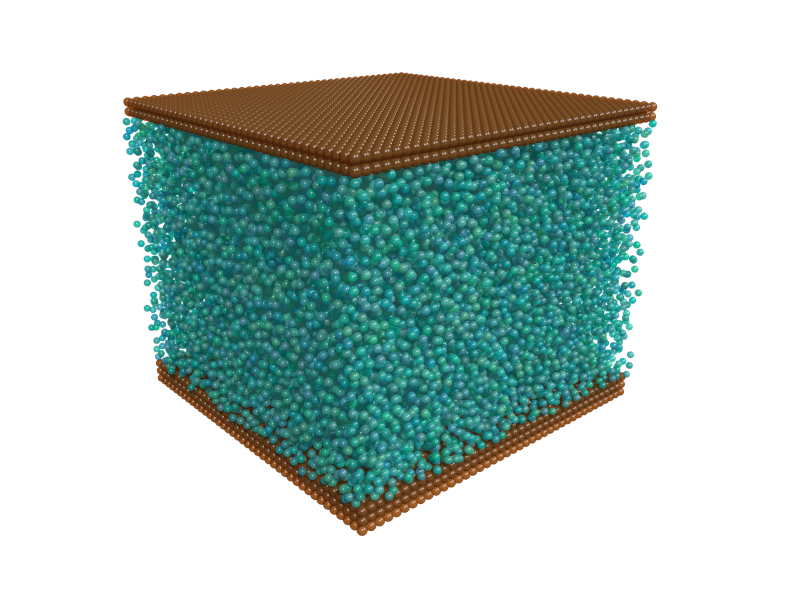
\includegraphics[width=.35\linewidth]{PRL3_gold2_wo_layers_wo_diffuse}
%    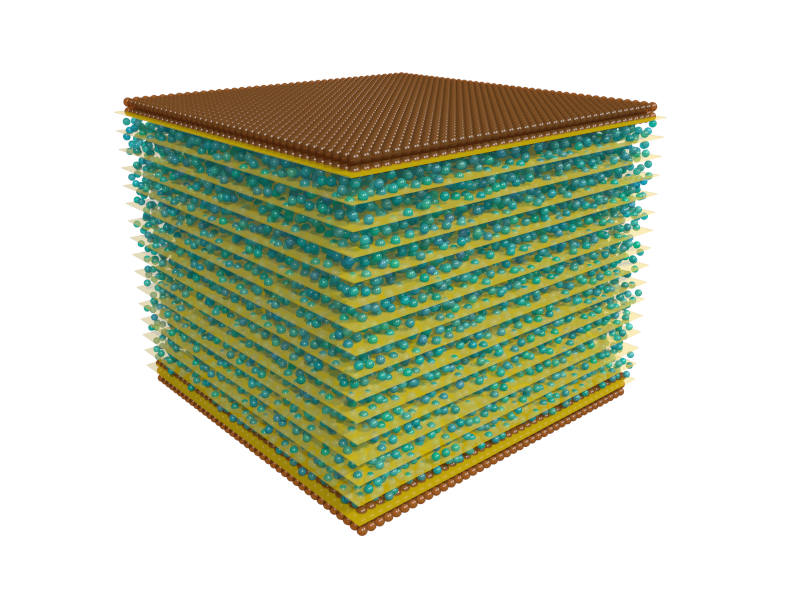
\includegraphics[width=.35\linewidth]{PRL3_gold2_wo_diffuse}
%      \end{center}
%    \item The characteristic function $\chi_\mu(z)$ and the finite element linear basis function $\Phi_\mu(z)$.
%  \begin{center}
%  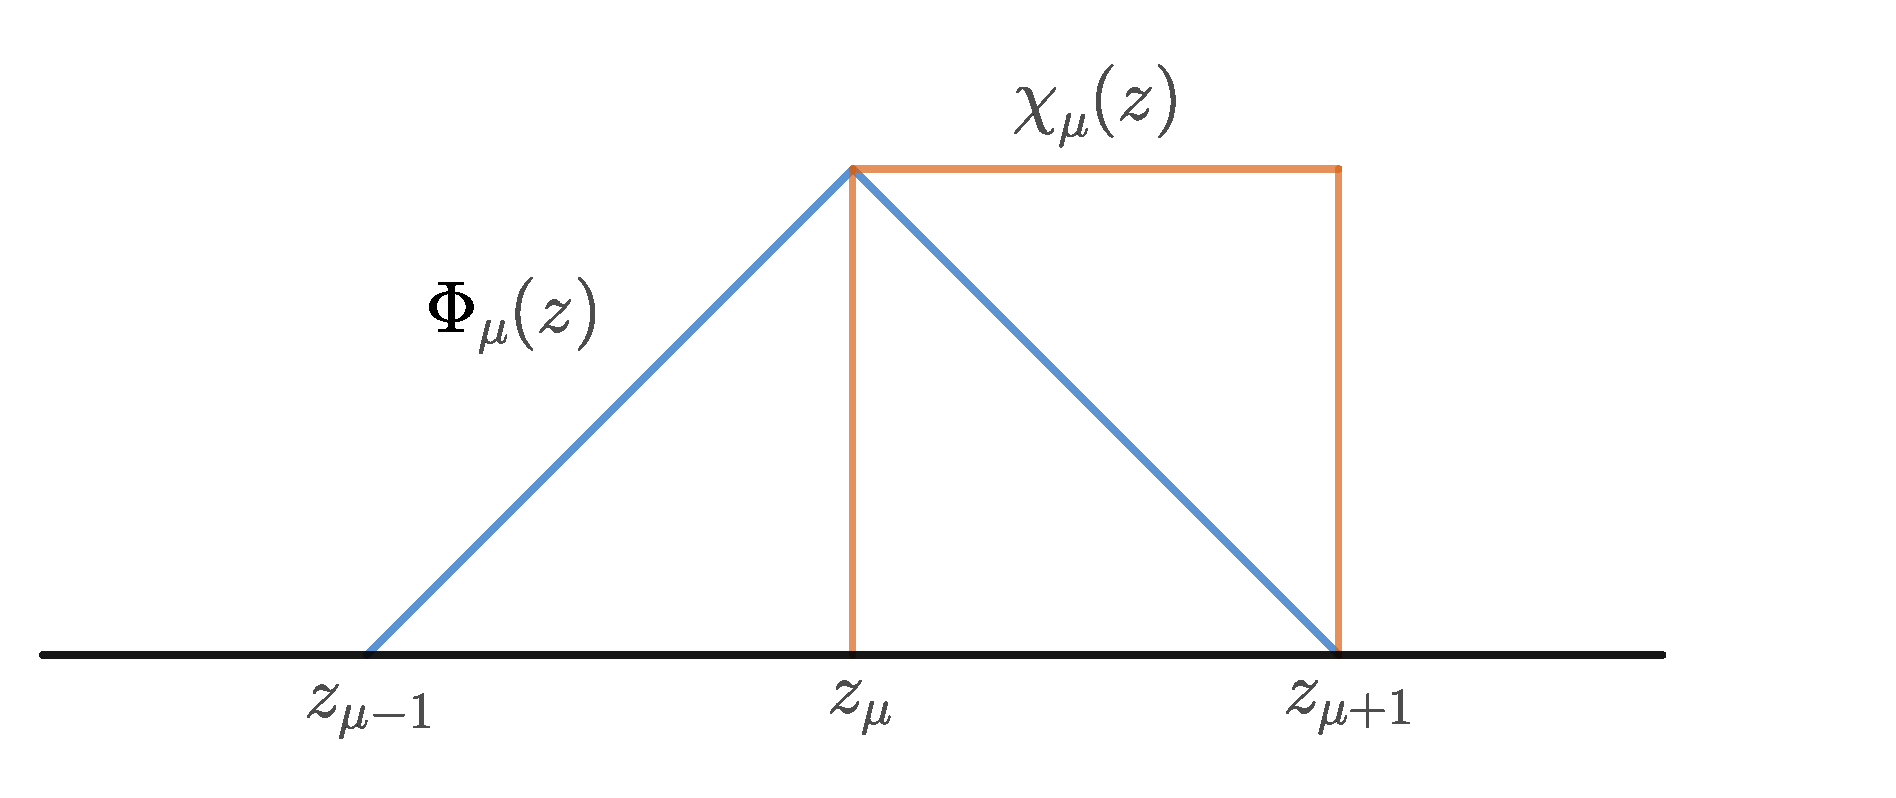
\includegraphics[scale=0.2]{psichi}
%\end{center}
%\end{itemize}
%\end{frame}
%
%\begin{frame}{The discrete basis function set}
%  \begin{itemize}
%    \item We can contruct \alert{continuum and discrete fields} from dual basis functions $\delta_{\mu}({\bf r})$ and $\psi_\mu({\bf r})$ 
%\begin{align}
%  v_\mu=\int d{\bf r}v({\bf r})\delta_\mu({\bf r}),&&
%    \overline{v}({\bf r}) =\sum_{\mu}v_\mu\psi_\mu({\bf r})
%\nonumber
%\end{align}
%\item
%The discrete  Dirac $\delta$ function is  defined in terms of  $\Phi_{\mu}(z)$
%\begin{align}
%  \delta_\mu({\bf r})\equiv\frac{\Phi_\mu({\bf r})}{{\cal V}_\mu}
%\nonumber
%\end{align}
%\item And the interpolant basis function takes the form
%  \begin{align}
%  \psi_\mu({\bf r})&
%  ={\cal V}_\mu \sum_\nu \left[M^{\Phi}\right]^{-1}_{\mu\nu} \Phi_\nu({\bf r})
%\nonumber
%\end{align}
%\item The usual mass matrix of the finite element method is 
%\begin{align}
%  M^\Phi_{\mu\nu}&=\int d{\bf r}\Phi_\mu({\bf r})\Phi_\nu({\bf r})
%\nonumber
%\end{align}
%\end{itemize}
%\end{frame}
%
%\begin{frame}{The discrete CG variables}
%  \begin{itemize}
%    \item The discrete CG variables
%\begin{align}
%  \hat{\rho}_\mu&= \sum_i^Nm_i\delta_\mu({\bf q}_i), &
%%\nonumber\\
%\hat{\bf g}_\mu&= \sum_i^N{\bf p}_i\delta_\mu({\bf q}_i)
%\nonumber
%\end{align}
%    \item The time derivatives
%\begin{align}
%  i{\cal L}  \hat{\rho}_{\mu}&=\sum_{i=1}^N{\bf p}_i\esc\boldsymbol{\nabla}\delta_\mu({\bf q}_i),&
%%\nonumber\\
%i{\cal L}  \hat{\bf g}_{\mu}&=\sum_{i=1}^N{\bf p}_i{\bf v}_i\esc\boldsymbol{\nabla}\delta_\mu({\bf q}_i)
%+\hat{\bf F}_\mu
%\nonumber
%\end{align}
%  \end{itemize}
%\end{frame}
%
%\begin{frame}{The discrete equations of nanohydrodynamics}
%  \begin{itemize}
%    \item The equation for the \alert{density}
%      \begin{align}
%\frac{d}{dt}\rho_\mu=&  \llg\overline{\rho} \; \overline{v}^{z}{\nabla}^{z}\delta_\mu \rlg
%        \nonumber
%      \end{align}
%    \item The \alert{normal component of the momentum}
%      \begin{align}
%    \frac{d}{dt}{{\bf g}}^{z}_\mu=&
%\llg\overline{\rho}\; \overline{v}^{z}\;\overline{v}^{z}{\nabla}^{z}\delta_{\mu}\rlg
%-\llg\overline{\rho}\delta_{\mu}{\nabla}^{z}\delta_{\nu}\rlg
%\frac{\partial  F}{\partial \rho_{\nu}}(\rho)
%+M_{\mu\nu}^{\bot}{\cal V}_\nu\tilde{v}^{z}_\nu
%\nonumber
%\end{align}
%\item The dissipative matrix is defined as
%\begin{align}
%M^{\bot}_{\mu\nu} 
%=&-\frac{\eta^\bot_{\mu\nu}-\eta^\bot_{\mu-1\nu}-\eta^\bot_{\mu\nu-1}+\eta^\bot_{\mu-1\nu-1}}{\Delta z^2}
%\nonumber \\
%&+\frac{{G}^\bot_{\mu\nu}-{G}^\bot_{\mu\nu-1}}{\Delta z}
%+\frac{{H}^\bot_{\mu\nu}-{H}^\bot_{\mu-1\nu}}{\Delta z}
%-{\gamma}^\bot_{\mu\nu}
%\nonumber
%\end{align}
%
%\item The \alert{parallel component}  ${\bf g}^\alpha_\mu$ for $\alpha
%=x,y$  of  the  discrete  momentum density
%\begin{align}
%    \frac{d}{dt}{{\bf g}}^\alpha_\mu=&-M_{\mu\nu}^{||}{\cal V}_\nu\tilde{v}^\alpha_\nu
%\nonumber
%\end{align}
%\end{itemize}  
%\end{frame}
%
%\begin{frame}{The transport kernels}
%\begin{align}
%\eta^{||}_{\mu\nu}&
%=\frac{1}{k_BT}\int_0^\tau  dt\left\langle 
%{\cal Q}\hat{\boldsymbol{\sigma}}^{xz}_\mu(t){\cal Q}\hat{\boldsymbol{\sigma}}^{xz}_\nu
%\right\rangle&&
%%\nonumber\\
%\eta^{\bot}_{\mu\nu}
%= \frac{1}{k_BT}\int_0^\tau  dt\langle 
%{\cal Q}\hat{\boldsymbol{\sigma}}^{zz}_\mu(t)
%{\cal Q}\hat{\boldsymbol{\sigma}}^{zz}_\nu\rangle
%\nonumber\\
%G^{||}_{\mu\nu}&
%=\frac{1}{k_BT} \int_0^\tau  dt
%\left\langle{\cal Q}\hat{\bf F}^{x}_\mu(t)
%{\cal Q}\hat{\boldsymbol{\sigma}}^{xz}_\nu
%\right\rangle&&
%%\nonumber\\
%G^{\bot}_{\mu\nu}=\frac{1}{k_BT} \int_0^\tau  dt
%\left\langle {\cal Q}\hat{\bf F}^{z}_\mu(t)
%{\cal Q}\hat{\boldsymbol{\sigma}}^{zz}_\nu
%\right\rangle
%\nonumber\\
%H^{||}_{\mu\nu}&
%=\frac{1}{k_BT} 
%\int_0^\tau  dt
%\left\langle{\cal Q}\hat{\boldsymbol{\sigma}}^{xz}_\mu(t){\cal Q}\hat{\bf F}^{x}_\nu\right\rangle&&
%%\nonumber\\
%H^\bot_{\mu\nu}=\frac{1}{k_BT} 
%\int_0^\tau  dt\left\langle {\cal Q}\hat{\boldsymbol{\sigma}}^{zz}_\mu(t){\cal Q}\hat{\bf F}^{z}_\nu\right\rangle
%\nonumber\\
%\gamma^{||}_{\mu\nu}&=
%\frac{1}{k_BT} \int_0^\tau  dt
%\left\langle 
%{\cal Q}\hat{\bf F}^{x}_\mu(t)
%{\cal Q}\hat{\bf F}^{x}_\nu\right\rangle&&
%%\nonumber\\
%\gamma^{\bot}_{\mu\nu}=
%\frac{1}{k_BT} \int_0^\tau  dt\left\langle 
%{\cal Q}\hat{\bf F}^{z}_\mu(t){\cal Q}\hat{\bf F}^{z}_\nu
%\right\rangle
%\nonumber
%\end{align}
%\end{frame}
%
%\begin{frame}{Summary}
%  \begin{itemize}
%    \item \alert{Isothermal hydrodynamic theory} for simple fluids in the presence of a solid sphere. 
%    \item Kawasaki-Gunton operator to obtain the evolution equations for the average of the CG variables. 
%    \item Markovian approximation: the CG variables should be slow in order to have memoryless equation. 
%    \item The theory describes the \alert{interaction fluid-solid} in terms of \alert{irreversible surfaces forces}.  
%    \item \alert{Hydrodynamic discrete theory for planar geometries} and flows involving discrete mass and momentum density variables defined in terms of finite element basis functions. 
%    \end{itemize}
%\end{frame}
%
%\section{The plateau problem and the corrected Green-Kubo formula}
%\begin{frame}{Plateau problem}
%  \begin{itemize}
%    \item Approximation of the linear integro-differential term 
%      \begin{align}
%  \frac{d}{dt}C(t)&=-L\esc C^{-1}(0)\esc C(t)
%        -\underbrace{\int_0^tdt' \Gamma(t-t')\esc C^{-1}(0)\esc  C(t')}_{M^* C^{-1}(0)C(t)=M^*c(t)}
%\nonumber
%\end{align}
%\item Rationale justifying the Markovian approximation 
%\begin{align}
%  \int_0^tdt' \Gamma(t-t')\esc c(t')&\simeq  \int_0^tdt' \Gamma(t-t')\esc  c(t)
%\equiv
%M^+(t)\esc c(t)
%\nonumber
%\end{align}
%%with the normalized correlation $c(t)$ as $C^{-1}(0)C(t)$.
%\item The \alert{projected} Green-Kubo running integral
%\begin{align}
%M^+(t)
%%&\equiv  \int_0^tdt' \Gamma(t') 
%%\nonumber\\
%& =\int_0^tdt' \llangle \left(\exp\{{\cal Q}i{\cal   L}t'\}{\cal Q}i{\cal L}\hat{A} \right){\cal Q} i{\cal L}\hat{A}^T\rrangle 
%\nonumber
%\end{align}
%\item The \alert{unprojected} Green-Kubo running integral is
%\begin{align}
%M(t)&\equiv  \int_0^{t} dt' \llangle \left(\exp\{i{\cal   L}t'\}i{\cal L}\hat{A} \right){\cal Q} i{\cal L}\hat{A}^T\rrangle
%\nonumber
%\end{align}
%\end{itemize}
%\end{frame}
%
%\begin{frame}{Plateau problem}
%  \begin{itemize}
%    \item After performing the running integrals
%\begin{align}
%M^+(t)&=
%  \llangle\left(\exp\{{\cal Q}i{\cal L}t\}  \hat{A}\right){\cal Q}i{\cal L}\hat{A}^{T} \rrangle
%\nonumber\\
%M(t)&=
%  \llangle\left(\exp\{i{\cal L}t\}  \hat{A}\right){\cal Q}i{\cal L}\hat{A}^{T} \rrangle
%\nonumber
%\end{align}
%\item $M^+(t)\approx M(t)$ when large separation of timescales. 
%\item $M(t)$ should have a plateau after a time $\tau$.
%\item For an ergodic system the correlations computed wiht the unprojected dynamics decay to zero
%\begin{align}
%  \lim_{t\to\infty}M(t)&= \lim_{t\to\infty} \llangle\left(\exp\{i{\cal L}t\}  \hat{A}\right){\cal Q}i{\cal L}\hat{A}^{T} \rrangle
%  \nonumber \\
%  &=
% \llangle  \hat{A}\rrangle\llangle{\cal Q}i{\cal L}\hat{A}^{T} \rrangle=0
% \nonumber
%\end{align}
%    \end{itemize}
%\end{frame}
%
%\begin{frame}{Corrected Green-Kubo formula}
%  \begin{itemize}
%    \item  
%Action  of Mori projector  operator on the phase  function $i{\cal
%  L}\hat{A}$
%\begin{align}
%{\cal Q} i{\cal L}\hat{A}  
%=
%i{\cal L}\hat{A}+L\esc C^{-1}(0)\esc \hat{A}  
%\nonumber
%\end{align}
%\item Therefore, we may express $M(t)$
%\begin{align}
%M(t)&=-\frac{d}{dt}C(t)-L\esc c(t)
%\nonumber
%\end{align}
%(Remember that $L=\langle \hat{A}i{\cal L}\hat{A}^T\rangle$)
%\item With $\frac{d}{dt}C(t)=-\lambda^*\cdot C(t)$ and $\lambda^*=(L+M*)\cdot C^{-1}(0)$ we obtain 
%\begin{align}
%M(\tau)&\simeq M^*\esc c(\tau)
%\nonumber
%\end{align}
%\item The \alert{new corrected Green-Kubo formula} does not suffer from the plateau problem by construction
%\begin{align}
%M^*&= \int_0^{\tau} dt \llangle {\cal Q} i{\cal L}\hat{A} (t)i{\cal L}\hat{A}^T\rrangle\esc  c^{-1}(\tau)
%\nonumber
%\end{align}
%\end{itemize}
%\end{frame}
%
%\begin{frame}{Corrected Green-Kubo formula}
%  \begin{itemize}
%\item We introduce the time dependent matrix 
%\begin{align}
%\Lambda(t)\equiv-    \frac{d}{dt}C(t)\esc C^{-1}(t)
%\nonumber
%\end{align}
%\item If the Markovian approximation is correct, after a time $\tau$, $\lambda(t)$ should become a time-independent matrix 
%\begin{align}
%  \lim_{t\to \infty}\Lambda(t)=\Lambda^*
%\nonumber
%\end{align}
%\item Therefore, the time-independent friction matrix $M^*$
%\begin{align}
%M^*&=  -L+ \Lambda^*\esc C(0)
%\nonumber
%\end{align}
%\end{itemize}
%\end{frame}
%
%\section{Space and time locality for unconfined fluids}
%\begin{frame}{The CG variables}
%\begin{figure}
%    \centering
%    \includegraphics[width=0.45\linewidth]{temp_wo_walls}
%    \includegraphics[width=0.45\linewidth]{temp_wo_walls_w_layers2}
%\end{figure}
%\begin{align}
%  \hat{\bf g}_\mu(z)= \sum_i^N{\bf p}_i\delta_\mu({\bf r}_i)&& 
%  i{\cal L}  \hat{g}_{\mu}(z)=-\frac{\hat{\sigma}^{xz}_{\mu}-\hat{\sigma}^{xz}_{\mu-1}}{\Delta z}
%\nonumber
%\end{align}
%\nonumber
%\end{frame}
%
%\begin{frame}{The Green-Kubo running integral $M(t)$ and $\eta(t)$}
%  \begin{itemize}
%    \item The Markovian dynamics given by Mori theory ($L=0$)
%\begin{align}
%    \frac{d}{dt}C(t) = -k_BTM^*\cdot c(t)
%    \nonumber
%\end{align}
%\item $M^*$ is related to the standard Green-Kubo running integral
%\begin{align}
%  M(t)&=\frac{1}{k_BT}\int_0^{t}dt' \llangle i{\cal L}\hat{g}(t')i{\cal L}\hat{g}^T\rrangle=-\frac{1}{k_BT}\frac{d}{dt}C(t)
%\nonumber
%\end{align}
%\item We may express $M(t)$ as $M(t)=-\Delta\cdot\eta(t)$, where $\Delta$ is the discrete Laplacian matrix and the nonlocal shear viscosity
%\begin{align}
%  \eta(t) &=\frac{1}{k_BT}\int_0^{t}dt' 
%  \llangle \hat{\sigma}^{xz}(t')\hat{\sigma}^{xz}\rrangle
%\nonumber
%\end{align}
%%\item Link between the momentum correlation matrix and the stress correlation matrix
%%\begin{align}
%%\frac{d}{dt}C(t)&= k_BT \Delta\esc \eta(t)
%%\nonumber
%%\end{align}
%\end{itemize}
%\end{frame}
%
%\begin{frame}{The friction matrix $M^*$ and the nonlocal shear viscosity matrix}
%\begin{itemize}
%\item Link between the momentum correlation matrix and the stress correlation matrix
%  \begin{align}
%  \frac{d}{dt}C(t)&= k_BT \Delta\esc \eta(t)
%  \nonumber
%  \end{align}
%\item By analogy
%  \begin{align}
%   M(t)=-\Delta\cdot\eta(t)&& \rightarrow &&M^*=-\Delta\cdot\eta^*
%  \nonumber
%  \end{align}
%\item The Markovian dynamics becomes
%  \begin{align}
%\frac{d}{dt}C(t)&=  k_BT\Delta\esc \eta^*\esc c(t)
%\nonumber
%\end{align}
%\item We would like to obtain $\eta^*$ from $\eta(t)$
%  \begin{align}
%    \Delta\cdot\eta(t)=\Delta\cdot\eta^*\cdot c(t)
%    \nonumber
%  \end{align}
%\item $\Delta$ and $c(t)$ are not invertible!
%\end{itemize}
%\end{frame}
%
%\begin{frame}{Fourier space}
%  \begin{itemize}
%    \item The unitay matrix and its inverse
%\begin{align}
%  E_{\mu\nu}&=\frac{1}{\sqrt{N_{\rm bin}}}\exp\left\{i\frac{2\pi}{N_{\rm bin}}\mu\nu\right\}
%  \nonumber \\
%  E^{-1}_{\mu\nu}&=\frac{1}{\sqrt{N_{\rm bin}}}\exp\left\{-i\frac{2\pi}{N_{\rm bin}}\mu\nu\right\}
%\nonumber
%\end{align} 
%    \item $E_{\mu}$ and $E_{\mu\nu}^{-1}$ diagonalizes any traslation invariant and periodic matrix $A_{\mu\nu}$
%      \begin{align}
%      \tilde{A}=E^{-1}\cdot A\cdot E
%      \nonumber
%    \end{align}
%  \end{itemize}
%\end{frame}
%
%\begin{frame}{The nonlocal viscosity and nonlocal kinematic viscosity}
%  \begin{itemize}
%  \item Therefore
%\begin{align}
%%  \frac{d}{dt}\tilde{C}(t)&=  k_BT\tilde{\Delta}\esc \tilde{\eta}^*\esc \tilde{c}(t)
%%\nonumber\\
%  \tilde{\Delta}\esc \tilde{\eta}(t) =\tilde{\Delta}\esc \tilde{\eta}^*\esc \tilde{c}(t)&& \rightarrow
%  &&\tilde{\eta}_{\mu\mu}^*=\frac{\tilde{\eta}_{\mu\mu}(t) }{\tilde{c}_{\mu\mu}(t)}
%\nonumber
%\end{align}
%%\item The eigenvalue $\tilde{\eta}_{00}$ is given by
%%\begin{align}
%%    \tilde{\eta}_{00}(t)=\frac{N_{\rm bin}}{V_T}\eta_0(t)
%%    \nonumber
%%\end{align}
%%  where the local shear viscosity is defined as
%%\begin{align}
%%  \eta_0(t) &\equiv \frac{V_T}{k_BT}\int_0^t dt'\llangle \hat{\sigma}_T^{xz}(t')\hat{\sigma}_T^{xz}
%%\rrangle
%%\nonumber
%%\end{align}
%\item The nonlocal kinematic viscosity is defined as
%\begin{align}
%\nu^*&\equiv  \eta^*\esc{\cal V}\esc \rho^{-1}
%\nonumber
%\end{align}
%where ${\cal V}$ is a diagonal matrix that contains the volume ${\cal V}_{\mu}$ of the bins and $\rho$ is the mass density matrix
%\item In Fourier space $\nu_{\mu}$ is a diagonal matrix
%\begin{align}
%  \tilde{\nu}_\mu^*&=  \frac{{\cal V}_\mu \tilde{\eta}_\mu^*}{\tilde{\rho}_\mu}
%  \nonumber
%\end{align}
%\item And the dynamic equation for the correlations
%  \begin{align}
%    \frac{d}{dt}C(t)=\Delta\cdot\nu^*\cdot C(t)
%    \nonumber
%  \end{align}
% \end{itemize}
% \end{frame}
%
%\begin{frame}{Local predictions}
%  \begin{itemize}
%
%\item The local approximation of the nonlocal viscosity matrix $nu$ is
%\begin{align}
%\nu_{\mu\mu'}&\simeq \nu_0 \delta_{\mu\mu'}
%  \nonumber
%\end{align}
%where the local kinematic viscosity is given by 
%\begin{align}
%\nu_0&\equiv \sum_{\mu'}\nu_{\mu\mu'} \quad \quad \quad\forall \mu
%\nonumber
%\end{align}
%\item Therefore, the \alert{local in space prediction}
%%\begin{align}
%%  \frac{d}{dt}{C}(t)=&\nu_0{\Delta}\esc { C}(t)
%%  \nonumber
%%\end{align}
%\begin{align}
%  C(t)&=\exp\left\{\Delta\esc \nu_0 (t-\tau) \right\}C(\tau)
%\nonumber
%\end{align}
%    \item The \alert{local in time prediction}
%\begin{align}
%  C(t)&=\exp\left\{\Delta\esc \nu^* (t-\tau) \right\}C(\tau)
%\nonumber
%\end{align}
%\end{itemize}
%\end{frame}
%
% \begin{frame}{Simulations}
%   \begin{enumerate}
%     \item Validation the Markovian approximation.
%     \item The nonlocal viscosity ($\eta(t)$ and $\eta^*(t)$). 
%     \item The nonlocal kinematic viscosity ($\nu(t)$ and $\nu^*(t)$). 
%     \item Prediction of the correlations (local and nonlocal). 
%   \end{enumerate}
% \end{frame}
%
% \begin{frame}{Simulation set up}
%   \begin{itemize}
%     \item Simulation of $28749$ particles interacting with a \alert{LJ potential} truncated at $\sigma=2.5$.
%     \item Box size $40x40x30$.
%     \item $dt=0.002$ in reduced units.
%     \item \alert{Equilibration stage}
%       \begin{itemize}
%         \item Langevin thermostat for $10^5$ timesteps: $T=2.0$, $\rho=0.6$.
%         \item NVE microcanonical conditions for a further $10^5$ timesteps.
%          \end{itemize}
%        \item \alert{Production stage}
%       \begin{itemize}
%         \item $1.5\times10^6$ timesteps.
%         \item $z$ axis binned in $60$ bins $\mu$. \alert{$\Delta z=0.5\sigma$}.
%         \item $g_{\mu}^x(t)$ and $\rho_{\mu}(t)$ recorded every $10$ timesteps. 
%         \end{itemize}
%     \end{itemize}
% \end{frame}
%
% \begin{frame}{The correlation matrix $C(t)$}
%   \begin{itemize}
% \item
%   The correlation matrix $C(t)$ at $t=0$ (left) and $t=0.6$ (right)
%\begin{figure}[h!]
%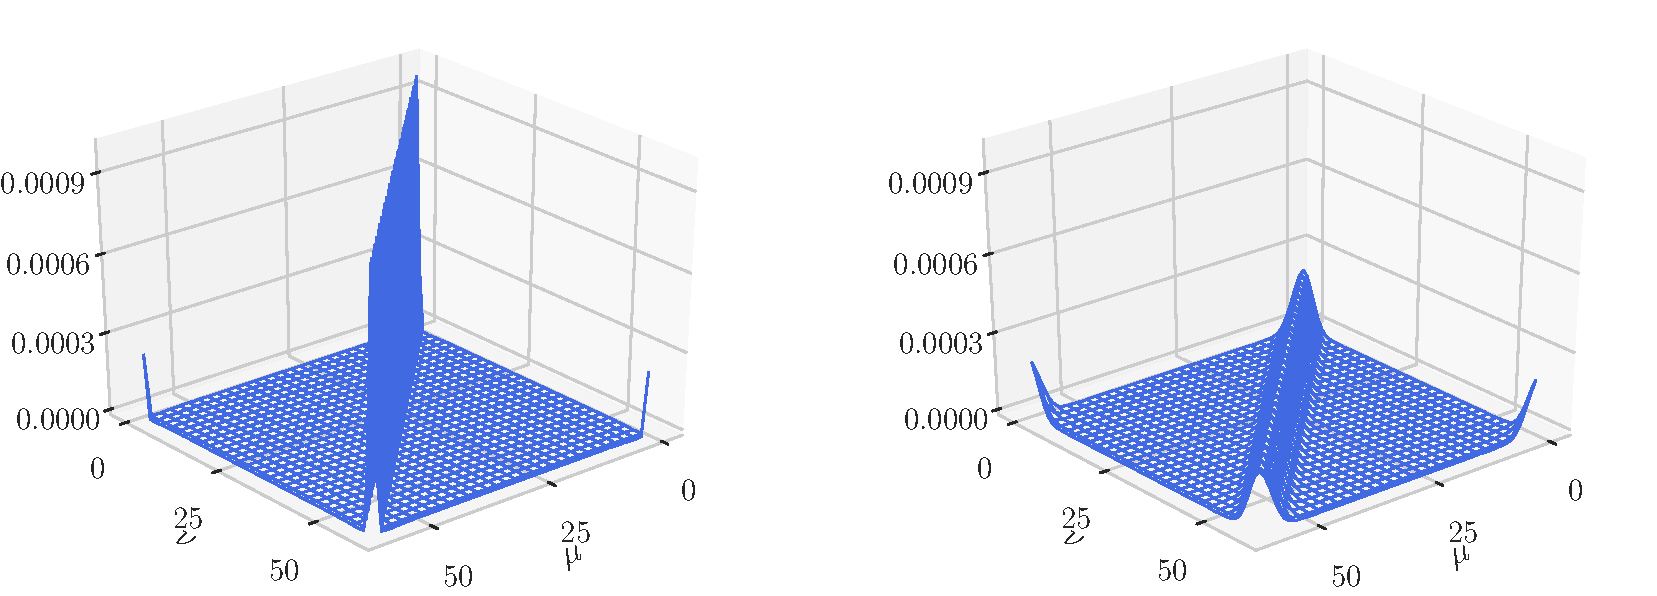
\includegraphics[width=\linewidth]{Ct-matrix-PBC}
%\end{figure}
%\item  The evolution of the different eigenvalues $\tilde{C}_{\mu\mu}(t)$. %The horizontal  line  at  the   value  $2\times10^{-5}$,  signaling  the
%  %threshold below which statistical errors give spurious results.
%\begin{figure}[h!]
%  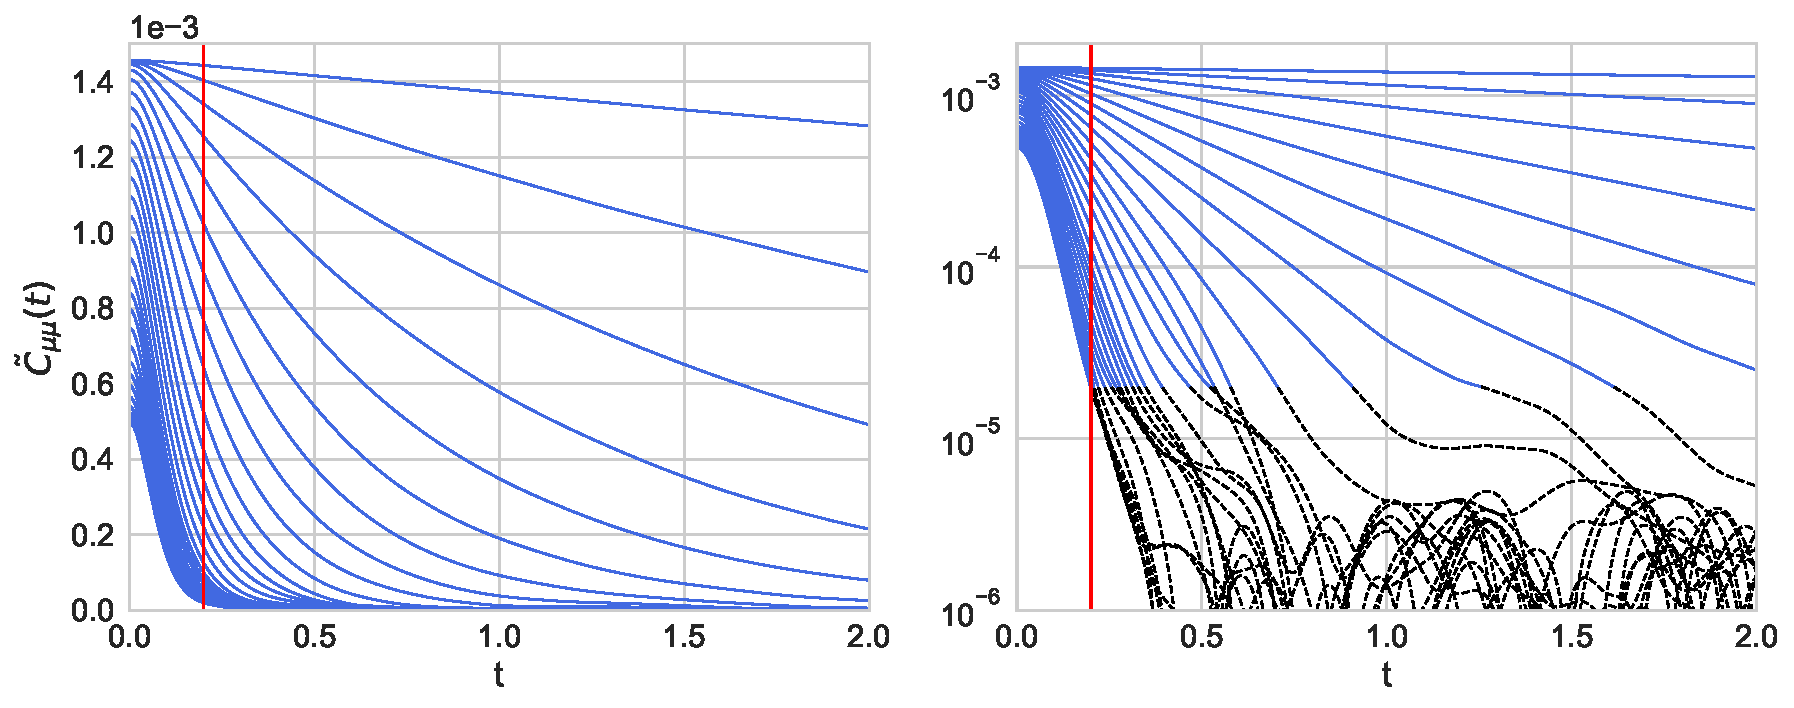
\includegraphics[width=\linewidth]{CtFourier-PBC-exp}
%\end{figure}
%\end{itemize}
%\end{frame}
%
%\begin{frame}{Validation of the Markovian approximation}
%\begin{figure}[h!]
%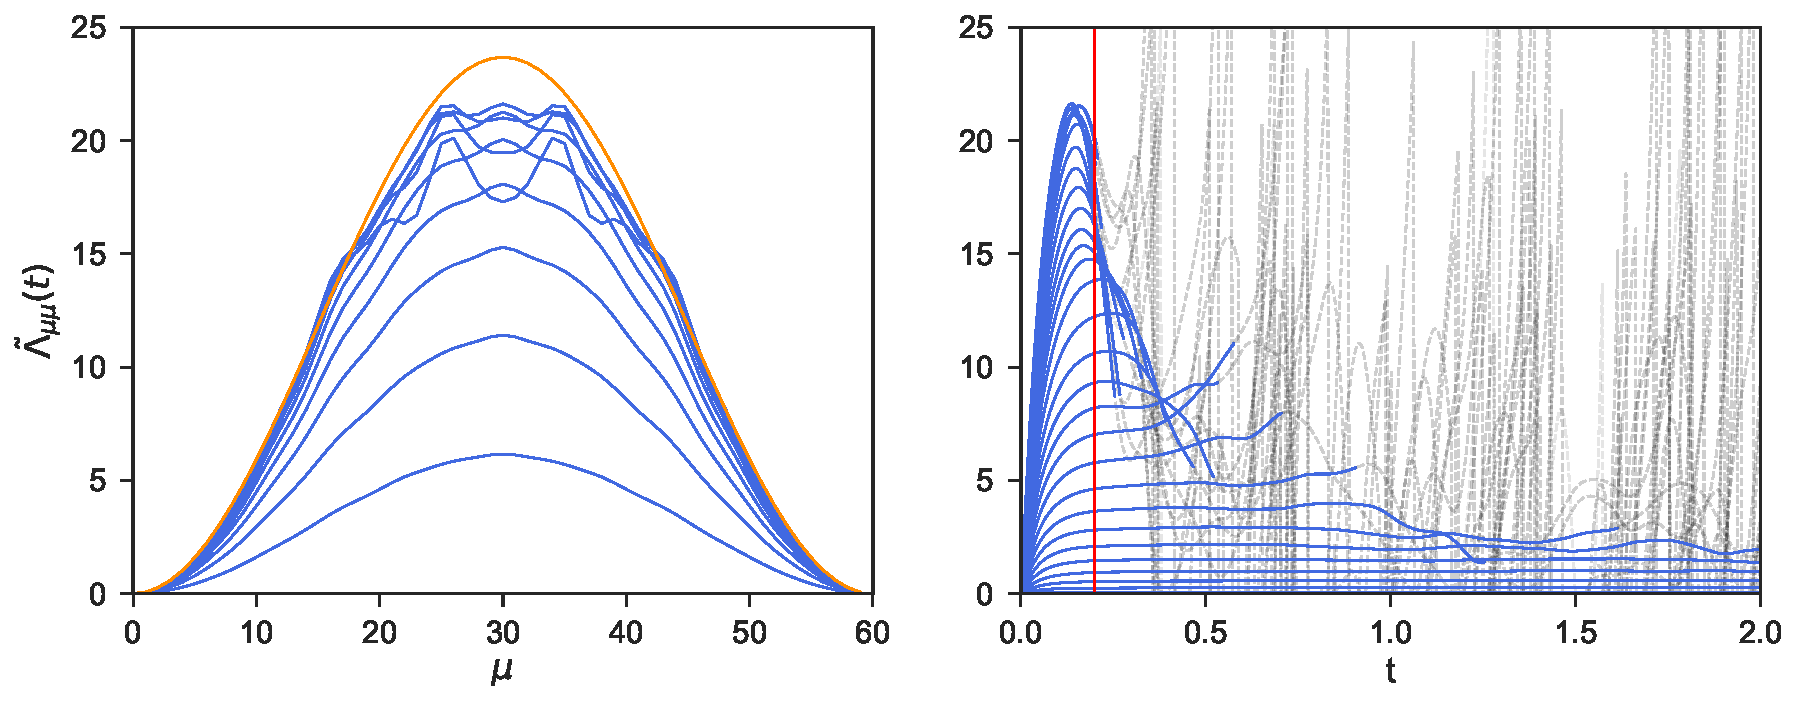
\includegraphics[width=\linewidth]{LambdatFourier-PBC}
%\end{figure}
%In  the left  panel, in
%  ascending  order the  plotted times  go  from $t=0$  to $t=0.20$  in
%  intervals of $0.02$.  The orange line is the local approximation
%  with a  value of the local  kinematic viscosity of
%  $\nu_0=1.48$.
% \end{frame}
%\begin{frame}{The nonlocal viscosity}
%\begin{figure}
%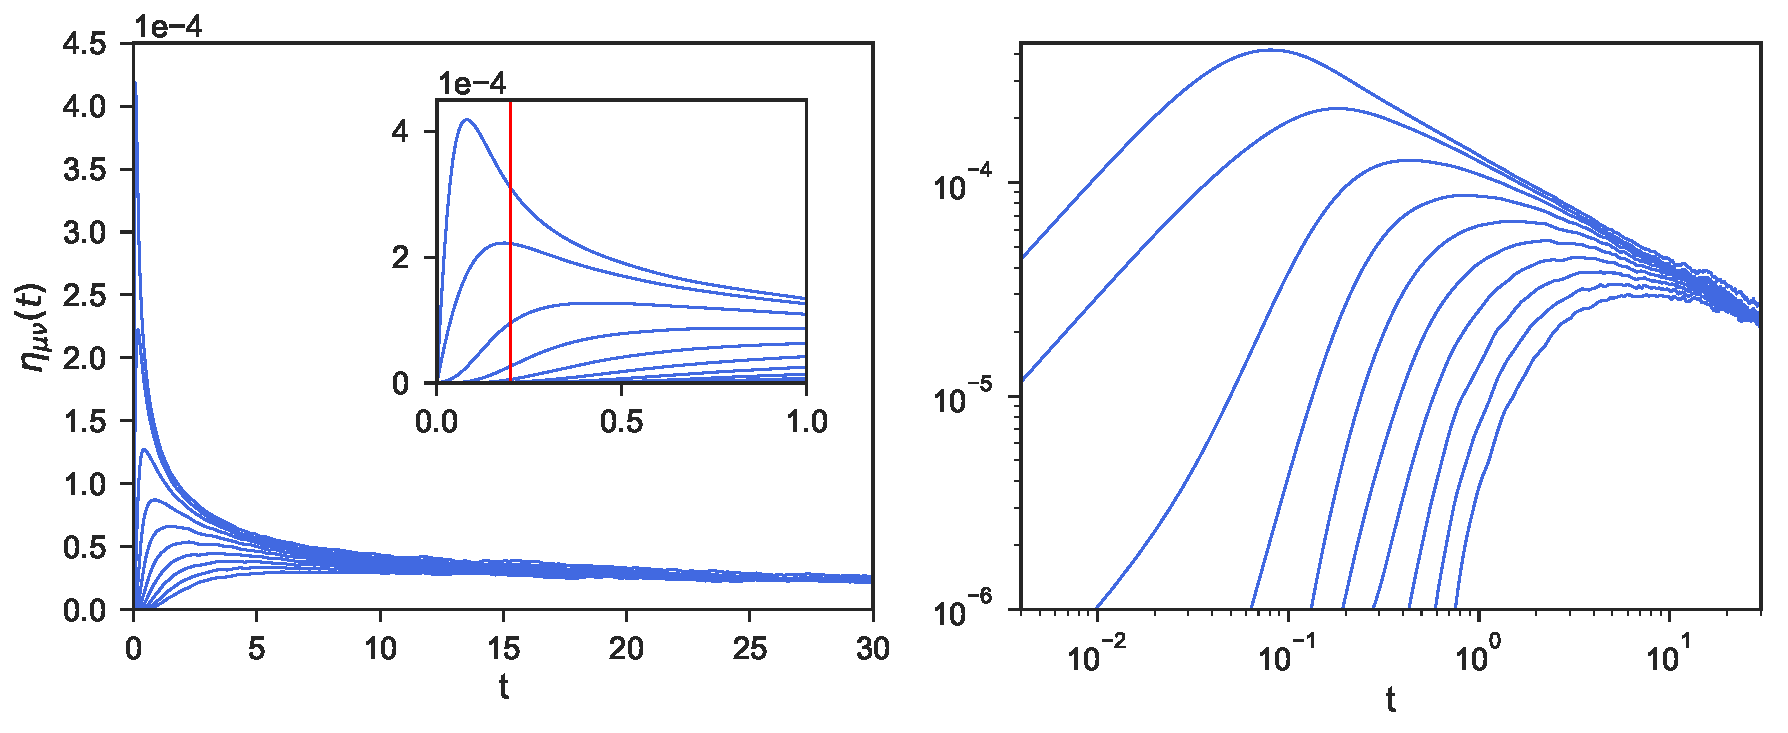
\includegraphics[width=\linewidth]{Etat-PBC}
%\end{figure}
%The nonlocal viscosity $\eta_{\mu\nu}(t)$ as a function of time, for $\mu=30$ and, in descending order, $\nu=30-40$. 
%\end{frame}
%
%\begin{frame}{The nonlocal viscosity $\tilde{eta}^*$}
%  \begin{align}
%  \tilde{\eta}^*_{\mu\mu}=\frac{\tilde{\eta}_{\mu\mu}(t)}{\tilde{c}_{\mu\mu}(t)}
%  \nonumber
%  \end{align}
%\begin{figure}[h!]
%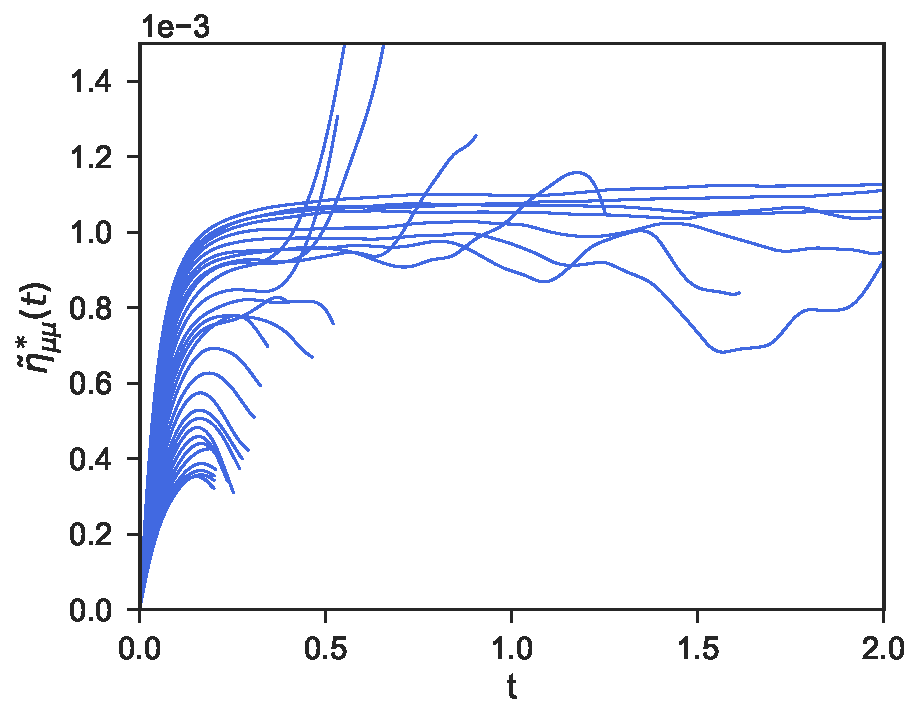
\includegraphics[width=0.5\linewidth]{EtaStartFourier-PBC}
%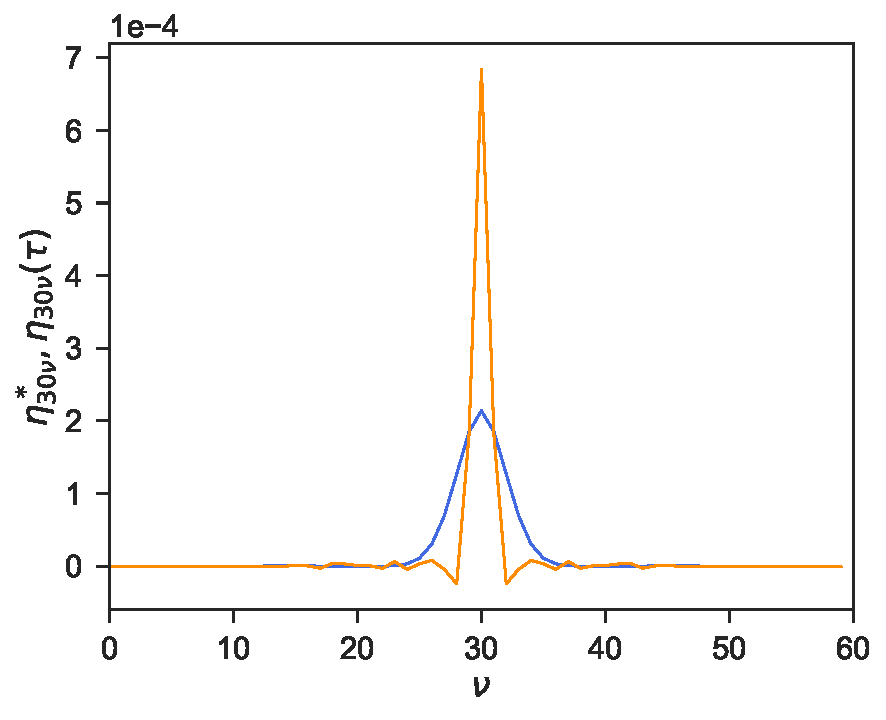
\includegraphics[width=0.5\linewidth]{CompareEtas-PBC}
%\end{figure}
%\end{frame}
%
%\begin{frame}{The nonlocal kinematic viscosity $\tilde{\nu}^*$}
%\begin{figure}[h!]
%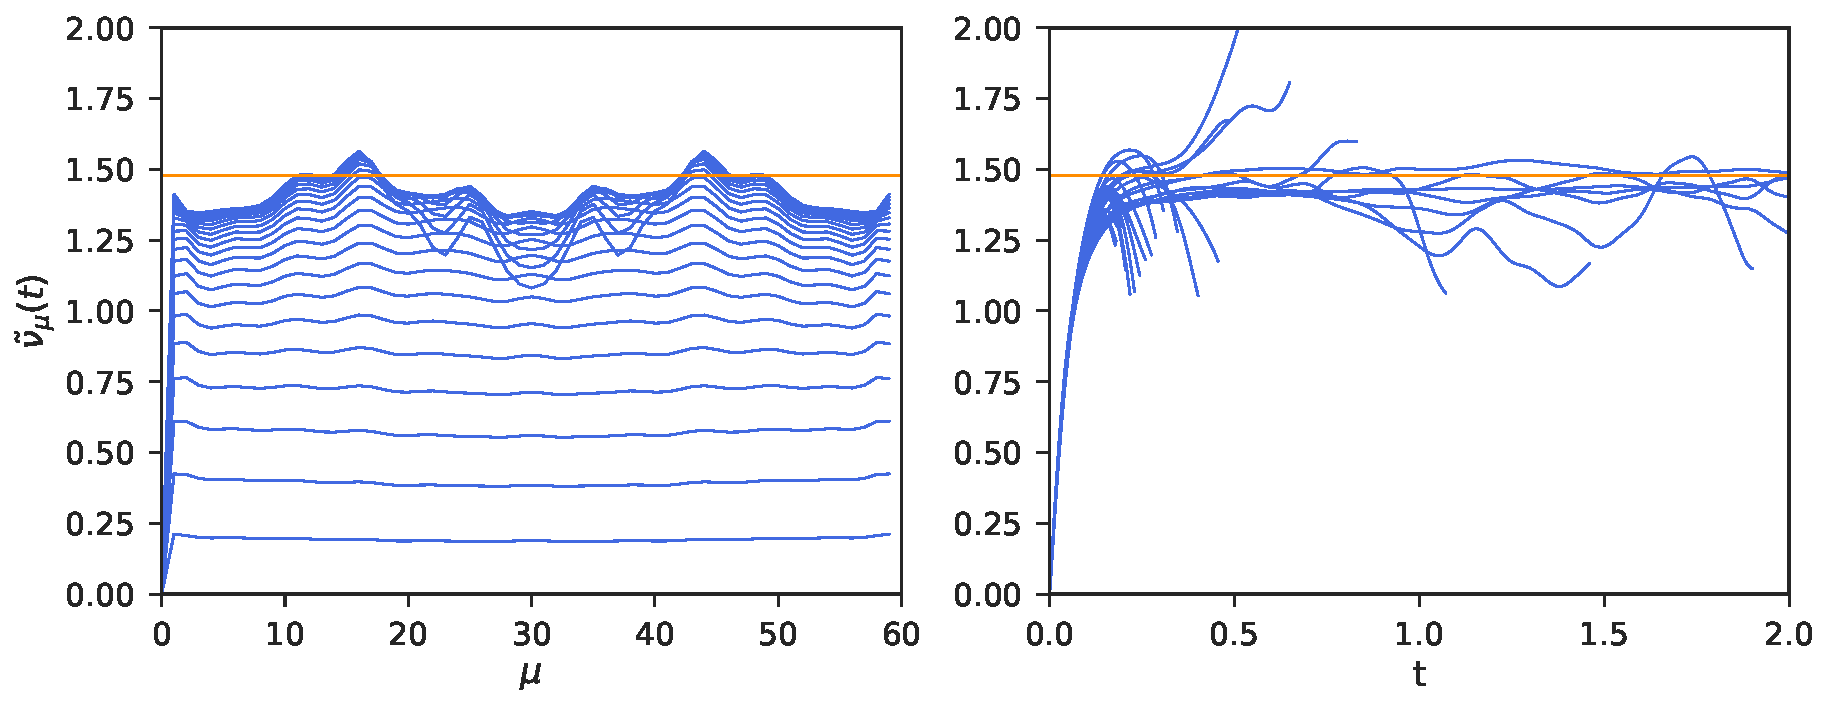
\includegraphics[width=\linewidth]{KinVisctFourier-PBC}
%\end{figure}
%The eigenvalues of the nonlocal kinematic viscosity matrix as a function of the mode index por times from $t=0$ to $t=0.2$ in ascending order in intervals of $0.01$. The orange line at $\nu_0=1.48$ is plotted in order to guide the eye in the plateau region.
%\end{frame}
%
%\begin{frame}{The local kinematic viscosity $\nu_0$}
%  \begin{align}
%    \nu_0(t)=\eta_0(t)/\rho^{\rm eq}
%    \nonumber
%  \end{align}
%\begin{figure}[h!]
%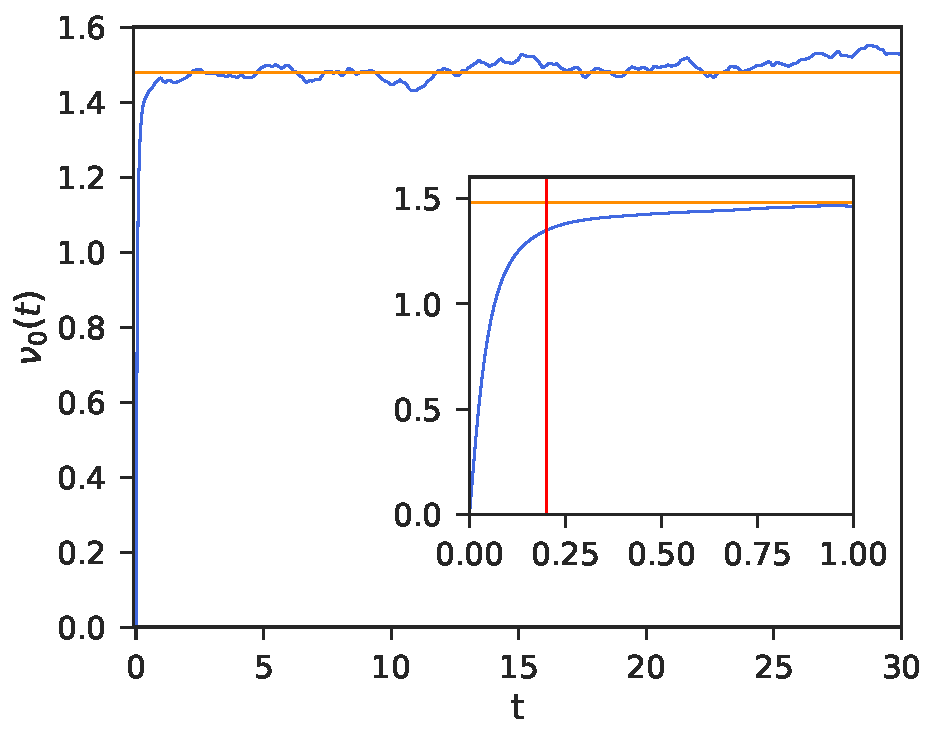
\includegraphics[scale=0.41]{KinVisc0t-PBC}
%\end{figure}
%The line at $\nu_0=1.48$ from the literature \cite{Woodcock2006}.
%\end{frame}
%
%\begin{frame}{Autocorrelation predictions $C_{\mu\mu}(t)$}
%\begin{figure}[h!]
%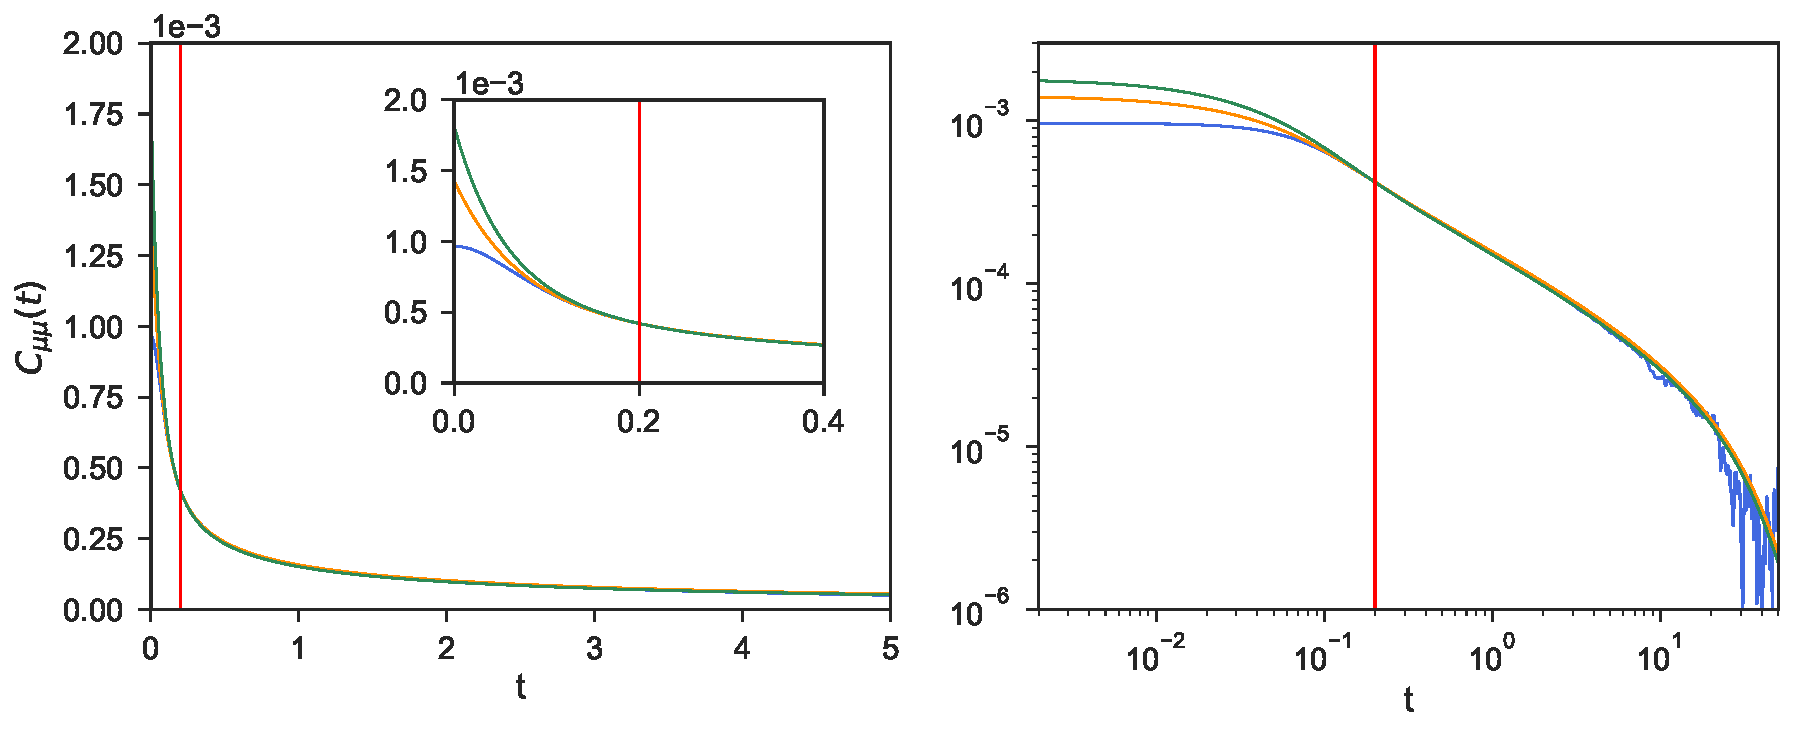
\includegraphics[width=\linewidth]{Predictionsmumu-PBC}
%\end{figure}
%{\color{blue} Blue}: Simulation results. \\
%{\color{orange} Orange}: nonlocal predictions.\\ 
%{\color{green} Green}: local predictions.\\
%\end{frame}
%
%\begin{frame}{Cross correlation predictions $C_{\mu\mu+1}(t)$}
%\begin{figure}[h!]
%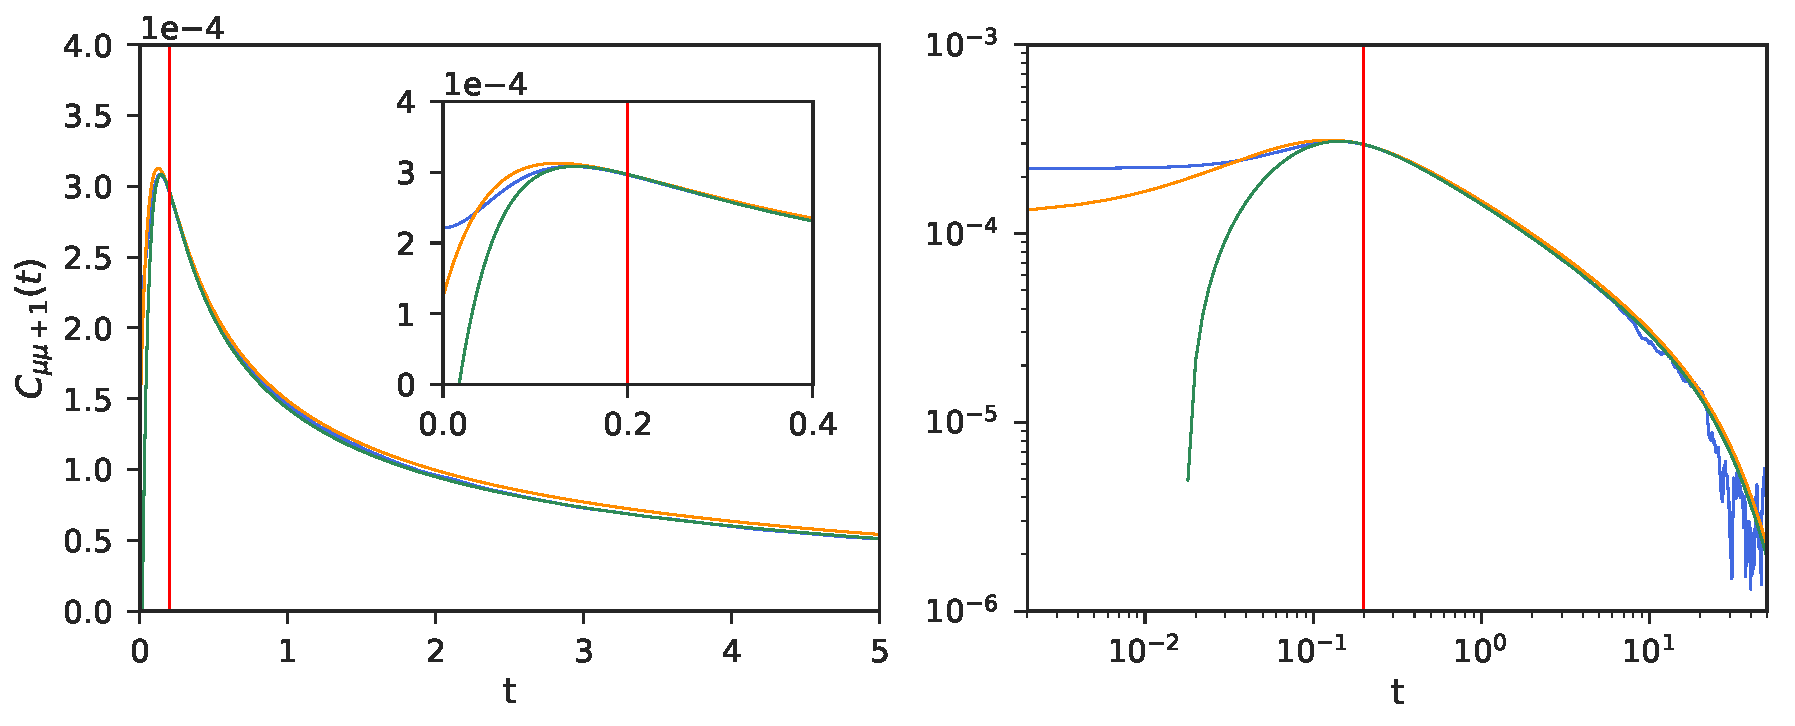
\includegraphics[width=\linewidth]{Predictionsmumu+1-PBC}
%\end{figure}
%{\color{blue} Blue}: Simulation results. \\
%{\color{orange} Orange}: nonlocal predictions.\\ 
%{\color{green} Green}: local predictions.\\
%\end{frame}
%
%\begin{frame}{Summary}
%  \begin{itemize}
%    \item Simple case: unconfined fluid.
%    \item Equation for the correlations
%      \begin{align}
%        \frac{d}{dt}C(t)=-k_BTM^*\cdot c(t)
%        \nonumber
%      \end{align}
%    \item Fourier space in order to observe a plateau in $\Lambda$ after a time $\tau=0.2$.
%    \item Plateau in the nonlocal viscosity $\tilde{\eta}^*$ and nonlocal kinematic viscosity $\tilde{\nu}^*$
%    \item Local kinematic viscosity $\nu_0$ equal to the value of the literature.
%    \item After a time $\tau=0.2$ the nonlocal aproximation and the local approximation gives us excelent results. 
%  \end{itemize}
%\end{frame}
%
%\section{Markovian behaviour near solids}
%\begin{frame}{The system and the CG variables}
%\begin{itemize}
%  \item The system
%\begin{figure}
%    \centering
%    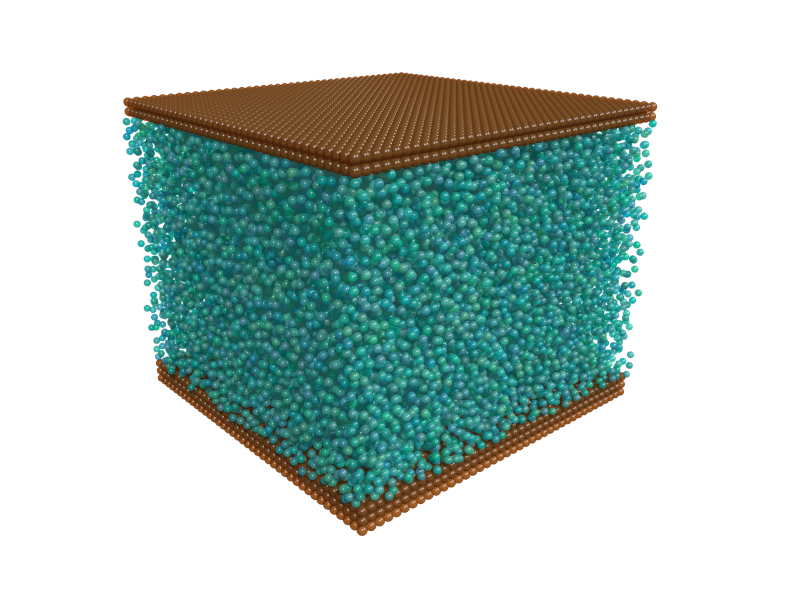
\includegraphics[width=0.45\linewidth]{PRL3_gold2_wo_layers_wo_diffuse}
%    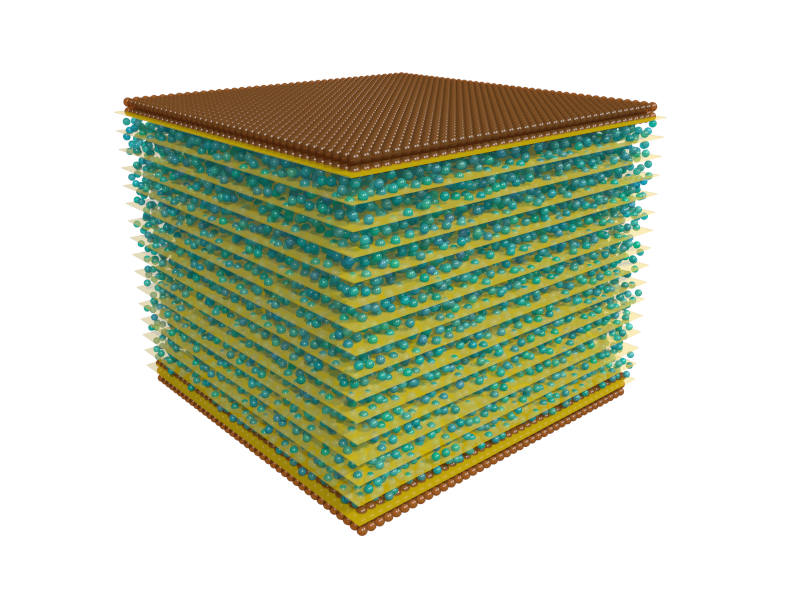
\includegraphics[width=0.45\linewidth]{PRL3_gold2_wo_diffuse}
%\end{figure}
%\item The CG variable and its correlation
%\begin{align}
%  \hat{\bf g}^x_\mu= \sum_i^N{\bf p}_i\delta_\mu({\bf q}_i), && 
%  \hat{g}^T=(\hat{\bf   g}^x_1,\cdots,\hat{\bf  g}^x_{N_{\rm   bin}}), &&
%  C(t)=\llangle \hat{g}(t) \hat{g}^T\rrangle 
%\nonumber
%\end{align}
%
%\item The predictions
%\begin{align}
%  C(t)^{\rm predict} = {\rm exp}{-\Lambda^*(t-\tau)}C(\tau)
%  \nonumber
%\end{align}
%\end{itemize}
%\end{frame}
%
%\begin{frame}{Reciprocal space}
%\begin{itemize}
%  \item Spectral decomposition
%\begin{align}
%  C(t)&=\sum_\mu^{N_{\rm bin}}\tilde{C}_\mu(t) u_\mu(t) \otimes u_\mu^T(t)
%\nonumber
%\end{align}
%
%\item The unitary matrix $E(t)$ diagonalizes the correlation matrix
%\begin{align}
%  E^{-1}(t)\esc C(t)\esc E(t)=\tilde{C}(t),
%\nonumber
%\end{align}
%
%\item Evolution of the diagonal matrix $\tilde{C}(t)$
%\begin{align}
%\frac{d}{dt}  \tilde{C}(t)&=-\tilde{\Lambda}^*\esc \tilde{C}(t)
%  +\frac{d }{dt}(E^{-1}(t)) \esc C(t)\esc E(t)
%  +E(t)\esc C(t)\esc \frac{d }{dt}E(t)  
%\nonumber
%\end{align}
%
%\item The time dependence of the unitary matrix if very weak
%\begin{align}
%\frac{d}{dt}  \tilde{C}(t)&\simeq-\tilde{\Lambda}^*\esc \tilde{C}(t)
%\nonumber
%\end{align}
%
%\item Evolution of the eigenvalues $\tilde{C}_{\mu}(t)$
%\begin{align}
%  \tilde{C}_\mu(t)&=\exp\{-\tilde{\Lambda}_{\mu\mu} (t-\tau)\}  \tilde{C}_\mu(\tau)
%  \nonumber
%\end{align}
%\end{itemize}
%\end{frame}
%
%\begin{frame}{Simulation set up}
%   \begin{itemize}
%     \item Simulation of $28175$ fluid particles interacting with a \alert{LJ potential} truncated at $\sigma=2.5$.
%     \item Two solid walls in the $xy$ plane confine the fluid.  
%     \item Box size $40x40x33$. 
%     \item $dt=0.002$ in reduced units.
%     \item \alert{Equilibration stage}
%       \begin{itemize}
%         \item Langevin thermostat for $10^5$ timesteps: $T=2.0$, $\rho=0.6$.
%         \item NVE microcanonical conditions for a further $10^5$ timesteps.
%          \end{itemize}
%        \item \alert{Production stage}
%       \begin{itemize}
%         \item $12\times10^6$ timesteps.
%         \item $z$ axis binned in $66$ bins $\mu$ \alert{$\Delta z=0.5\sigma$} or $33$ bins $\mu$ \alert{$\Delta z=2\sigma$}.
%         \item $g_{\mu}^x(t)$ recorded every $2$ timesteps. 
%         \end{itemize}
%     \end{itemize}
%\end{frame}
%
%\begin{frame}{Thin bins ($\Delta z=0.5\sigma$)}
%  \begin{itemize}
%    \item $C_{\mu\nu}(t)$ for  $t=0$ (left) and $t=0.6$ (right).
%\begin{figure}[h!]
%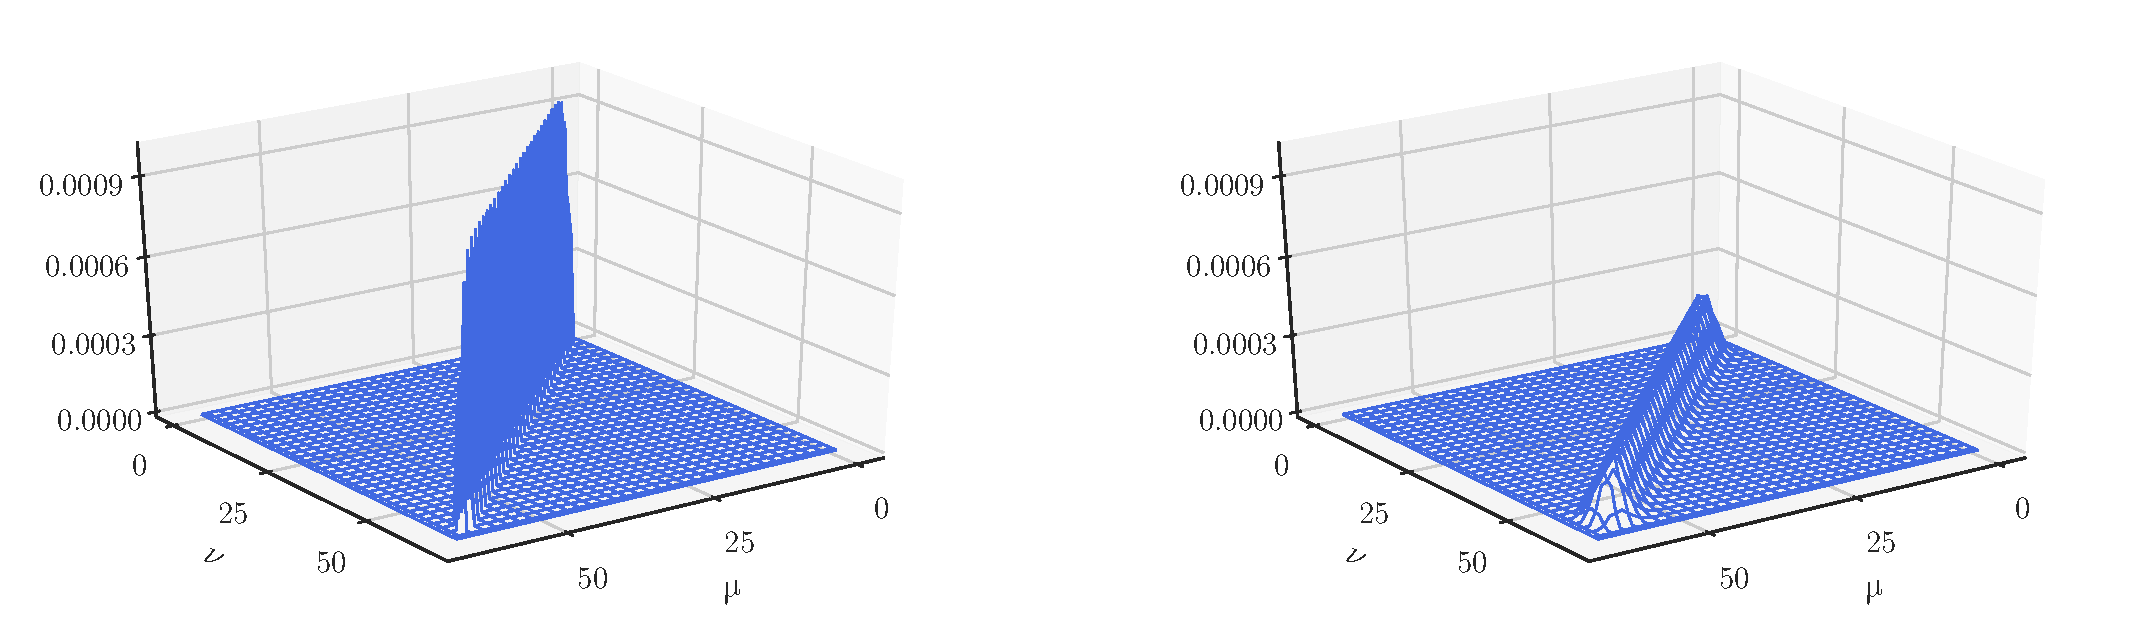
\includegraphics[width=\linewidth]{Ct-matrix-WALLS-66nodes}
%\end{figure}
%\item Evolution of different eigenvalues $\tilde{C}_{\mu\nu}(t)$
%\begin{figure}[h!]
%  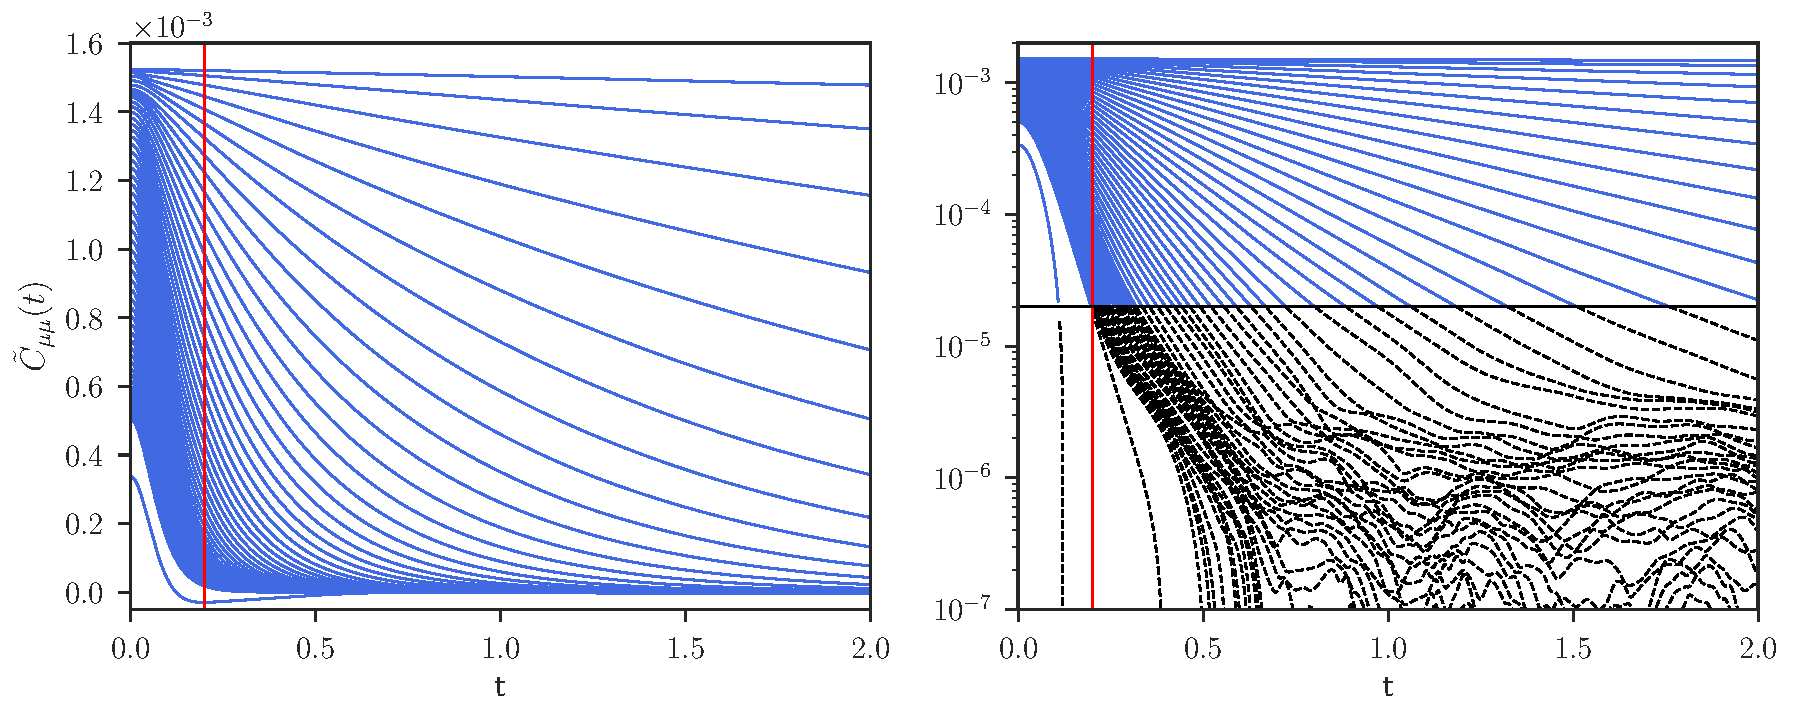
\includegraphics[width=\linewidth]{CtRec-WALLS-66nodes-exp}
%\end{figure}
%\end{itemize}
%\end{frame}
%
%\begin{frame}{$\tilde{\Lambda}(t)$ ($\Delta z=0.5\sigma$)}
%Diagonal elements  $\tilde{\Lambda}_{\mu\mu}(t)$ of $\Lambda(t)$ in the reciprocal space. After a time $\tau=0.2$ we observe a nice plateau for the lower modes. 
%\begin{figure}[h!]
%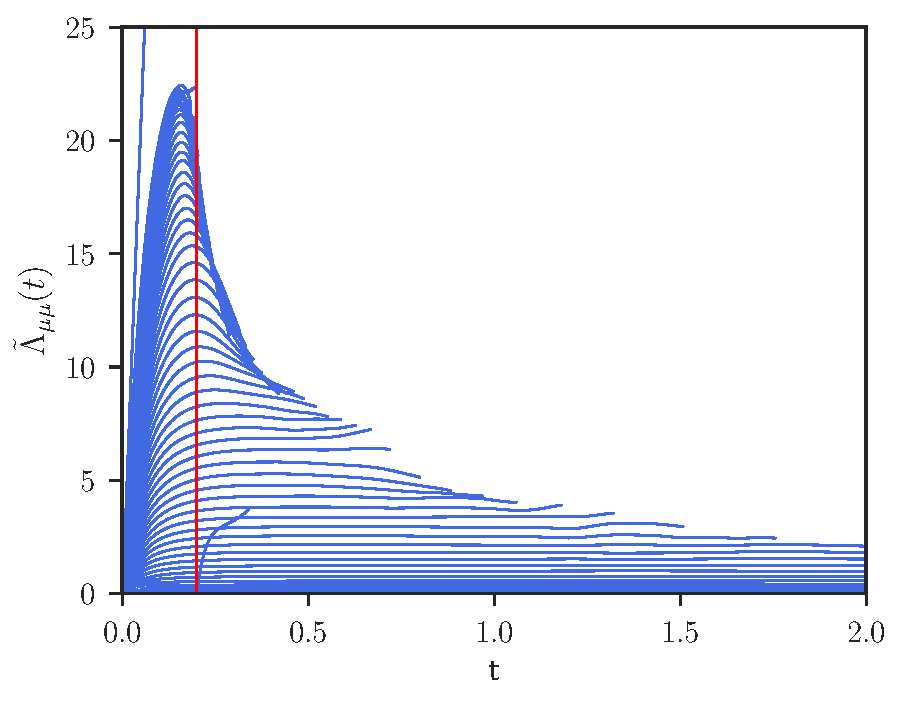
\includegraphics[scale=0.5]{LambdatRec-WALLS-66nodes}
%\end{figure}
%\end{frame}
%
%\begin{frame}{Eigenvalues and eigenvectors near the walls ($\Delta z=0.5\sigma$)}
%    The eigenvalues $\tilde{C}_{\mu}(t)$ of the correlation matrix $C(t)$ for $\mu=59,60$ which are identical and superimpose (left) and the corresponding eigenvectors $u_{\mu}$ in blue and orange, respectively (right).
%  \begin{figure}[h!]
%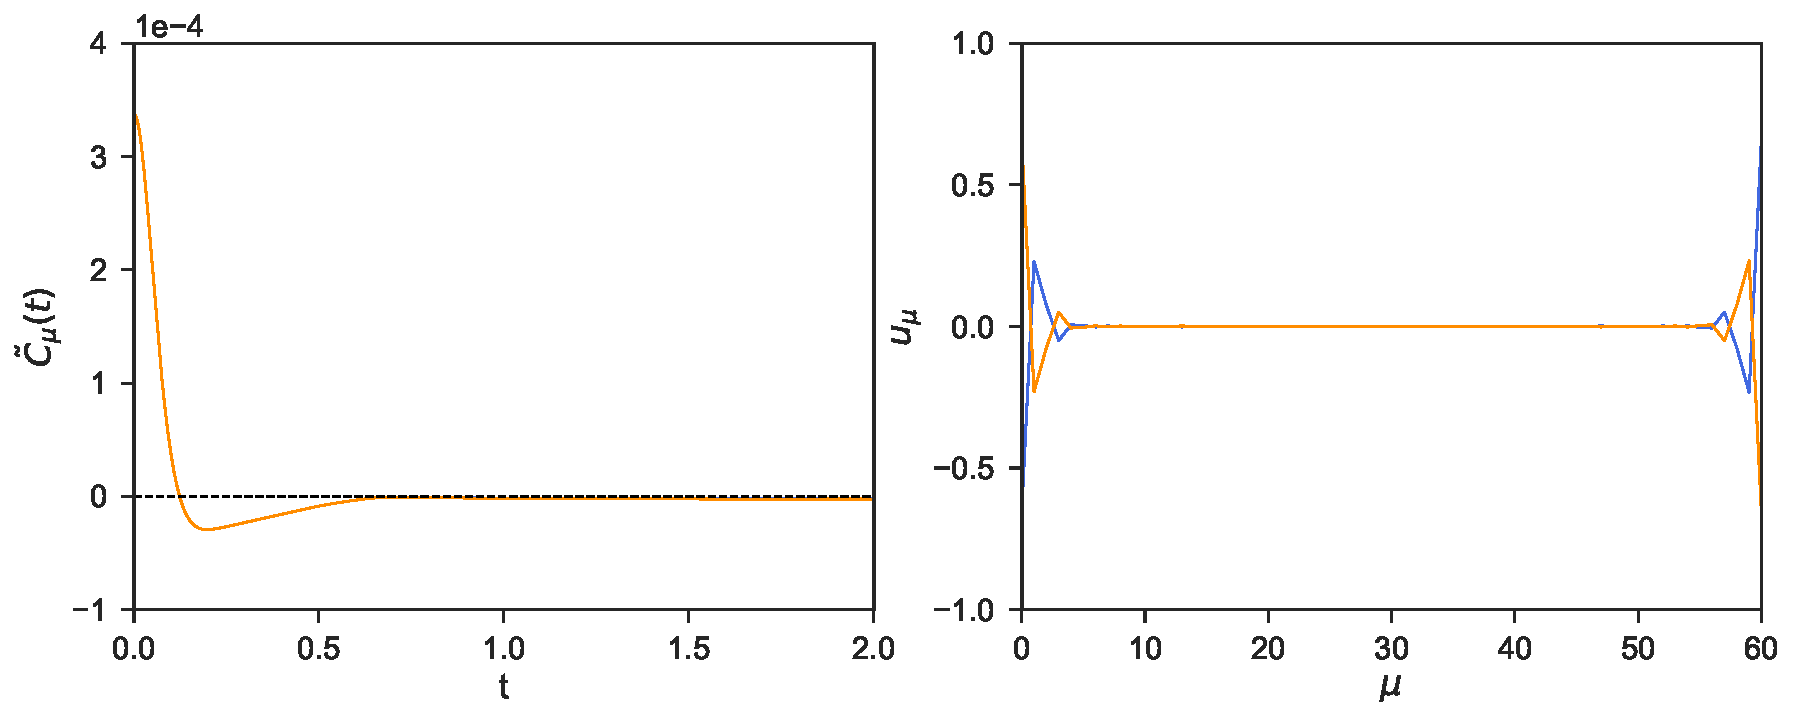
\includegraphics[width=\linewidth]{EigenvaluesVectors-WALLS-66nodes}
%\end{figure}
%\end{frame}
%
%\begin{frame}{Predicted correlations in the bulk ($\Delta z=0.5\sigma$)}
%  In the middle of the canal the predicted (orange) correlation fits perfectly the measured (blue) correlation after a time $\tau=0.2$
%\begin{figure}[h!]
%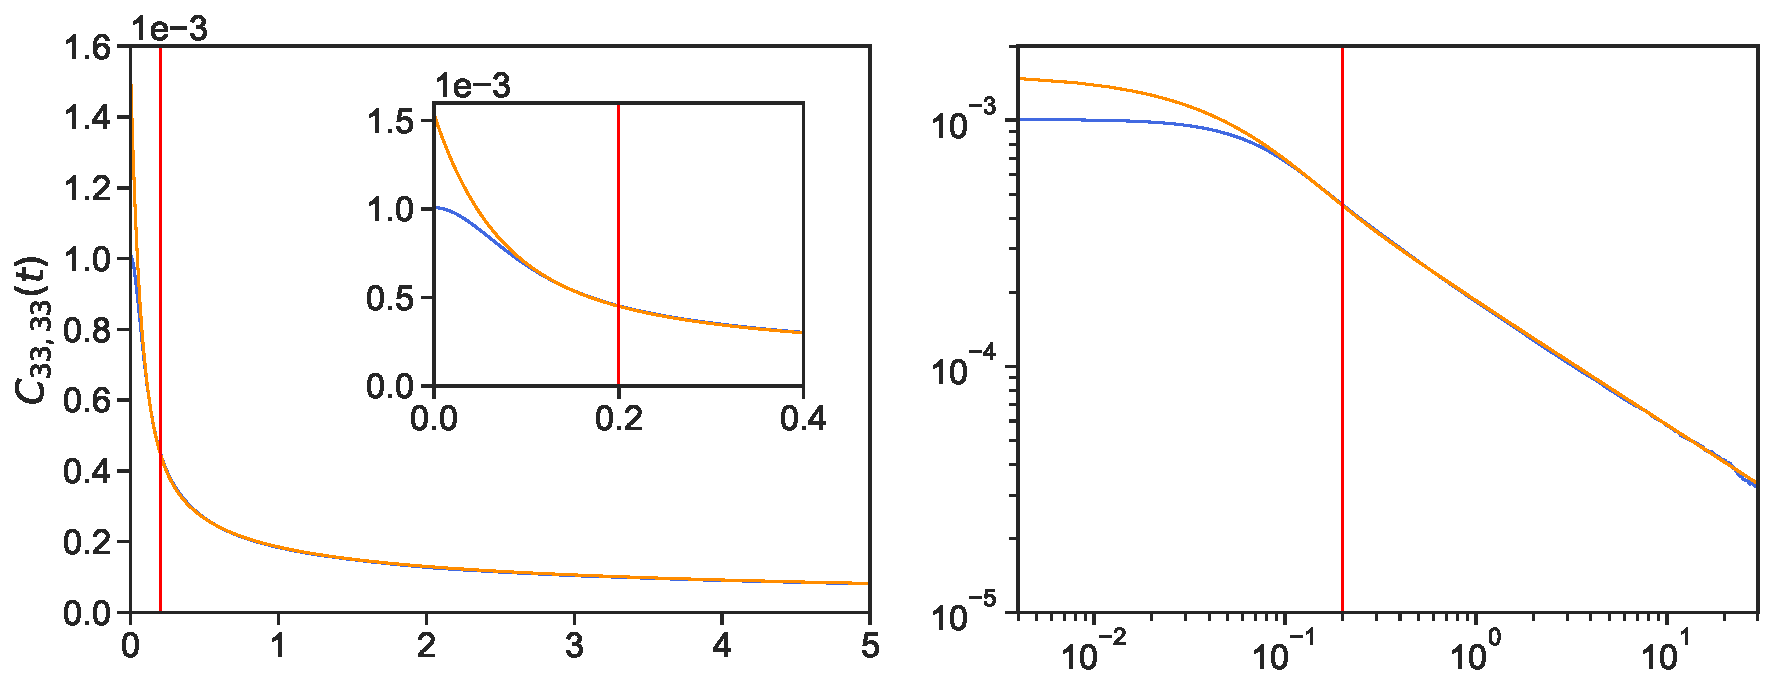
\includegraphics[width=\linewidth]{Predictions-canal-WALLS-66nodes-defense}
%\end{figure}
%\end{frame}
%
%\begin{frame}{Predicted correlations near the walls ($\Delta z=0.5\sigma$)}
%\begin{figure}[h!]
%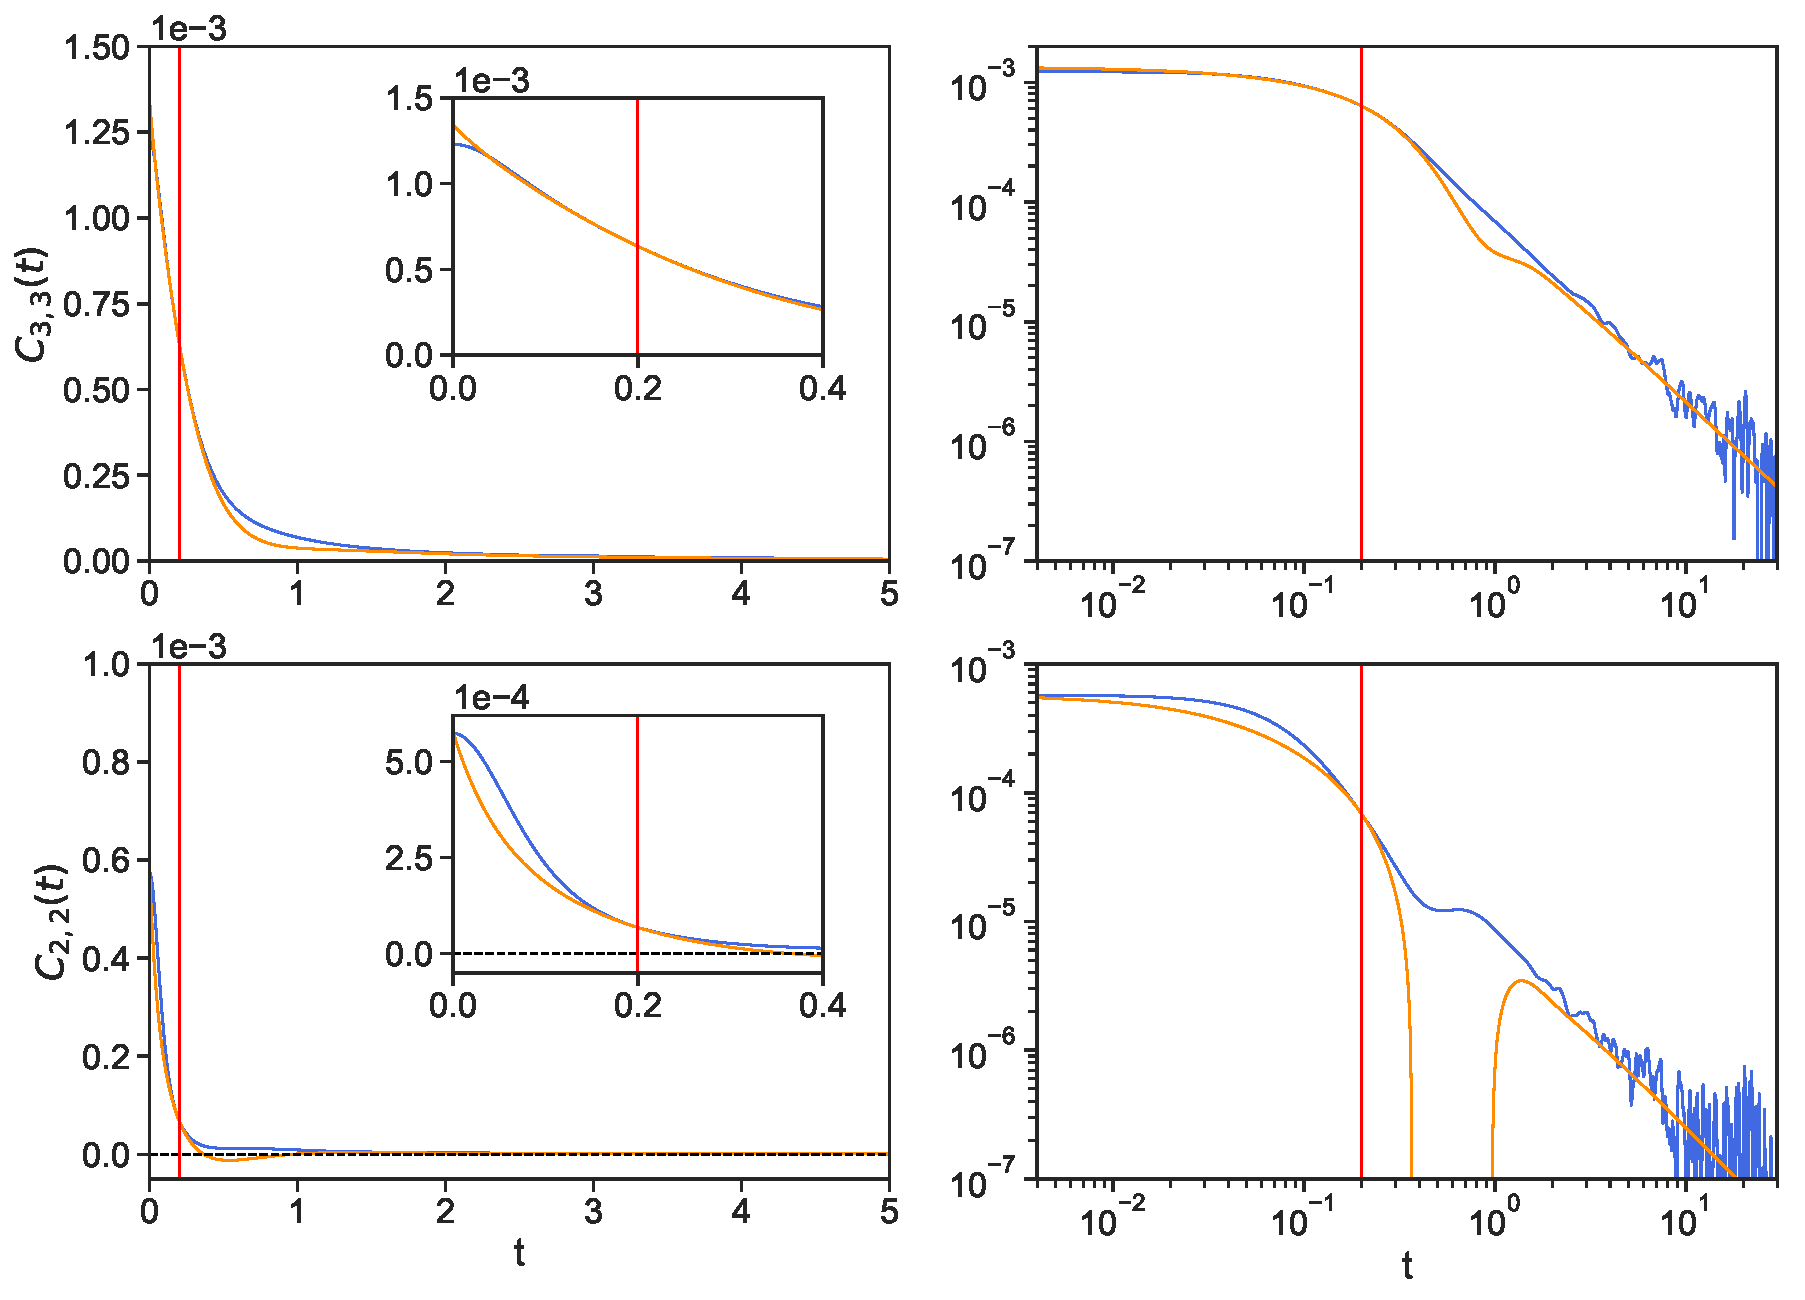
\includegraphics[width=\linewidth]{Predictions-WALLS-66nodes-defense}
%\end{figure}
%\end{frame}
%
%\begin{frame}{Eigenvalues $\tilde{C}_{\mu\mu}(t)$ ($\Delta=2\sigma$)}
%Evolution of different eigenvalues $\tilde{C}_{\mu\nu}(t)$. Also  plotted are  a vertical line  at $t=\tau=0.3$.
%\begin{figure}[h!]
%  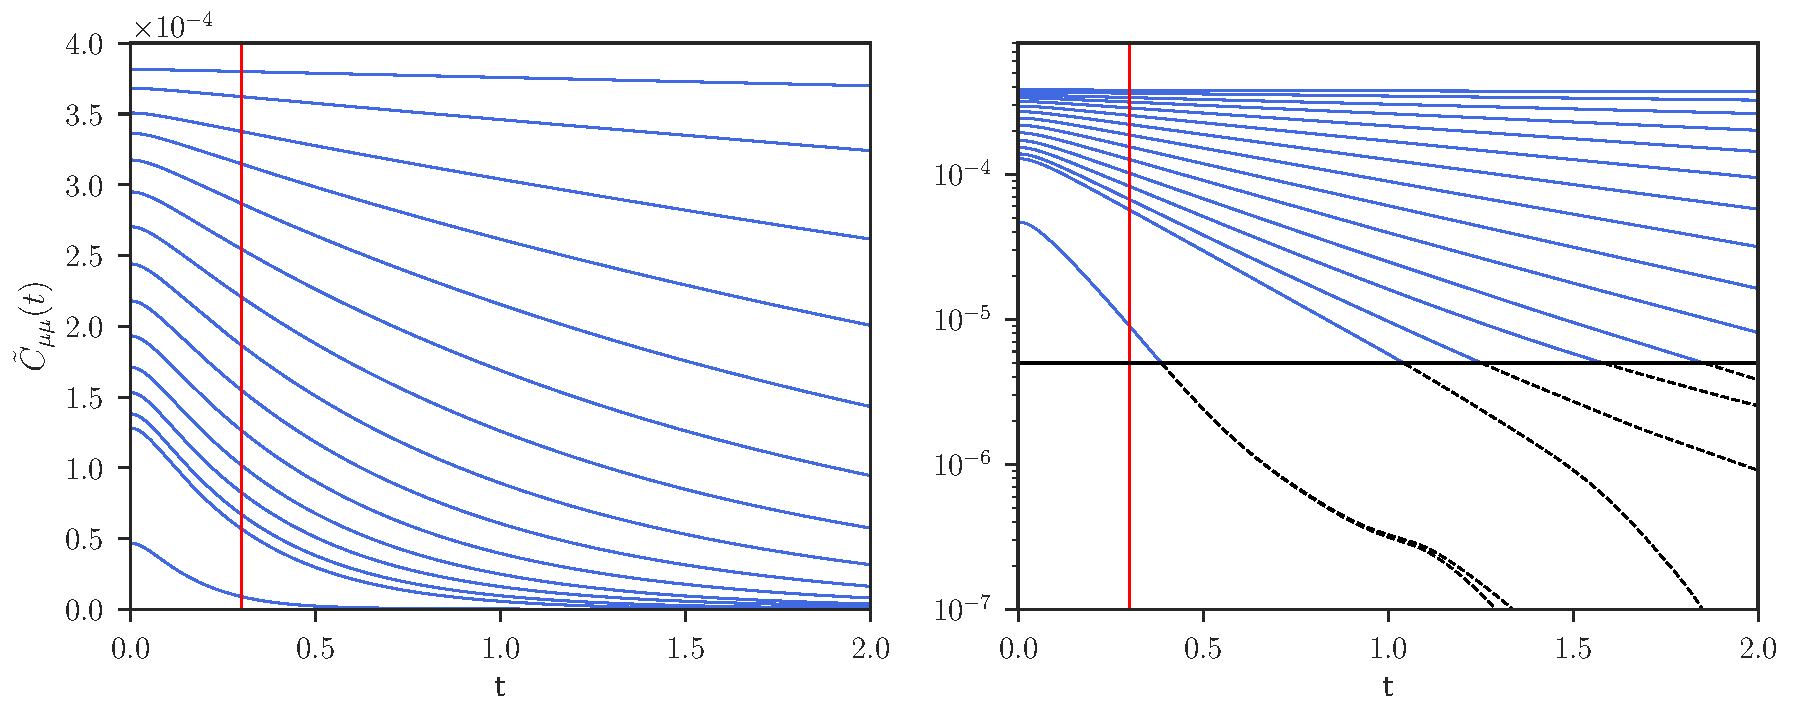
\includegraphics[width=\linewidth]{CtRec-WALLS-17nodes-exp}
%\end{figure}
%\end{frame}
%
%\begin{frame}{Eigenvectors near the walls ($\Delta z=2\sigma$)}
% The eigenvectors correspondings to the two largest eigenvalues of $\Lambda(t)$ for a confined fluid.
%  \begin{figure}[h!]
%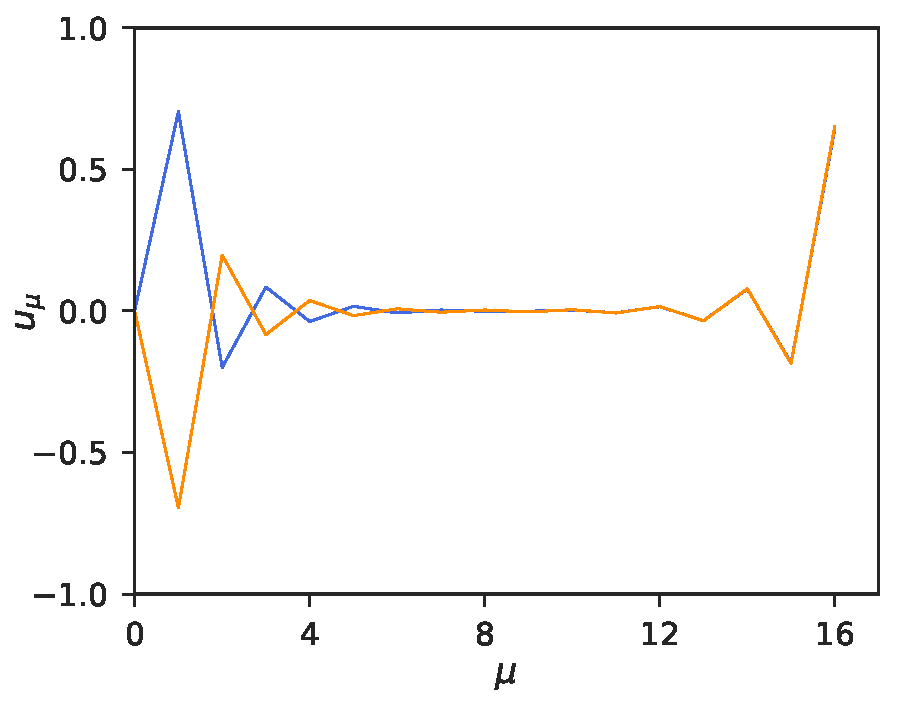
\includegraphics[scale=0.5]{Eigenvectors-WALLS-17nodes}
%\end{figure}
%\end{frame}
%
%\begin{frame}{$\tilde{\Lambda}(t)$ for thick bins ($\Delta z=2\sigma$)}
%    Diagonal elements  $\tilde{\Lambda}_{\mu\mu}(t)$ of $\Lambda(t)$ in the reciprocal space
%\begin{figure}[h!]
%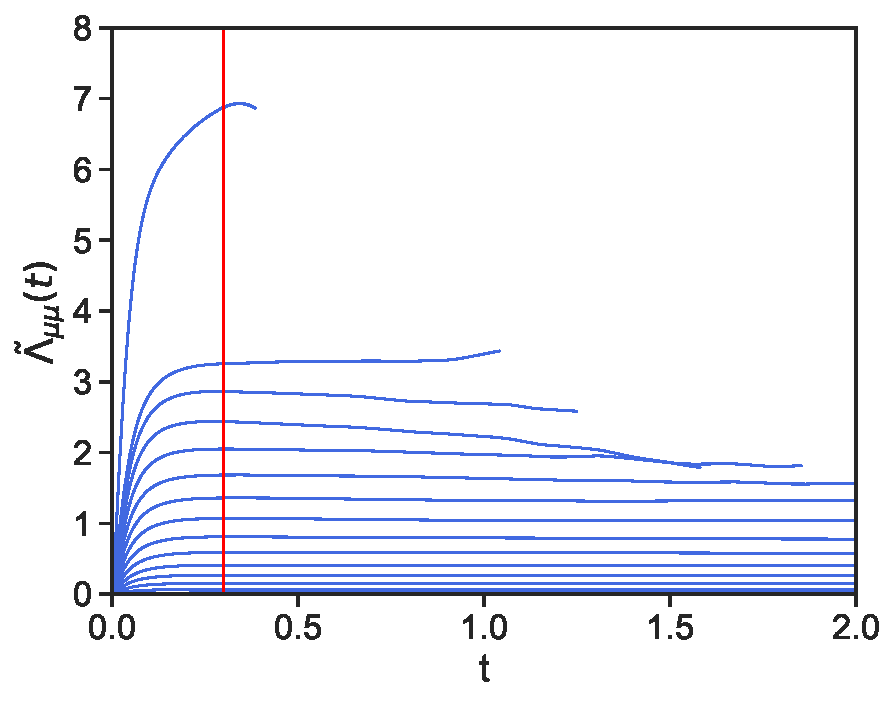
\includegraphics[scale=0.5]{LambdatRec-WALLS-17nodes}
%\end{figure}
%\end{frame}
%
%
%\begin{frame}{Predicted auto-correlations ($\Delta z=2\sigma$)}
%\begin{figure}[h!]
%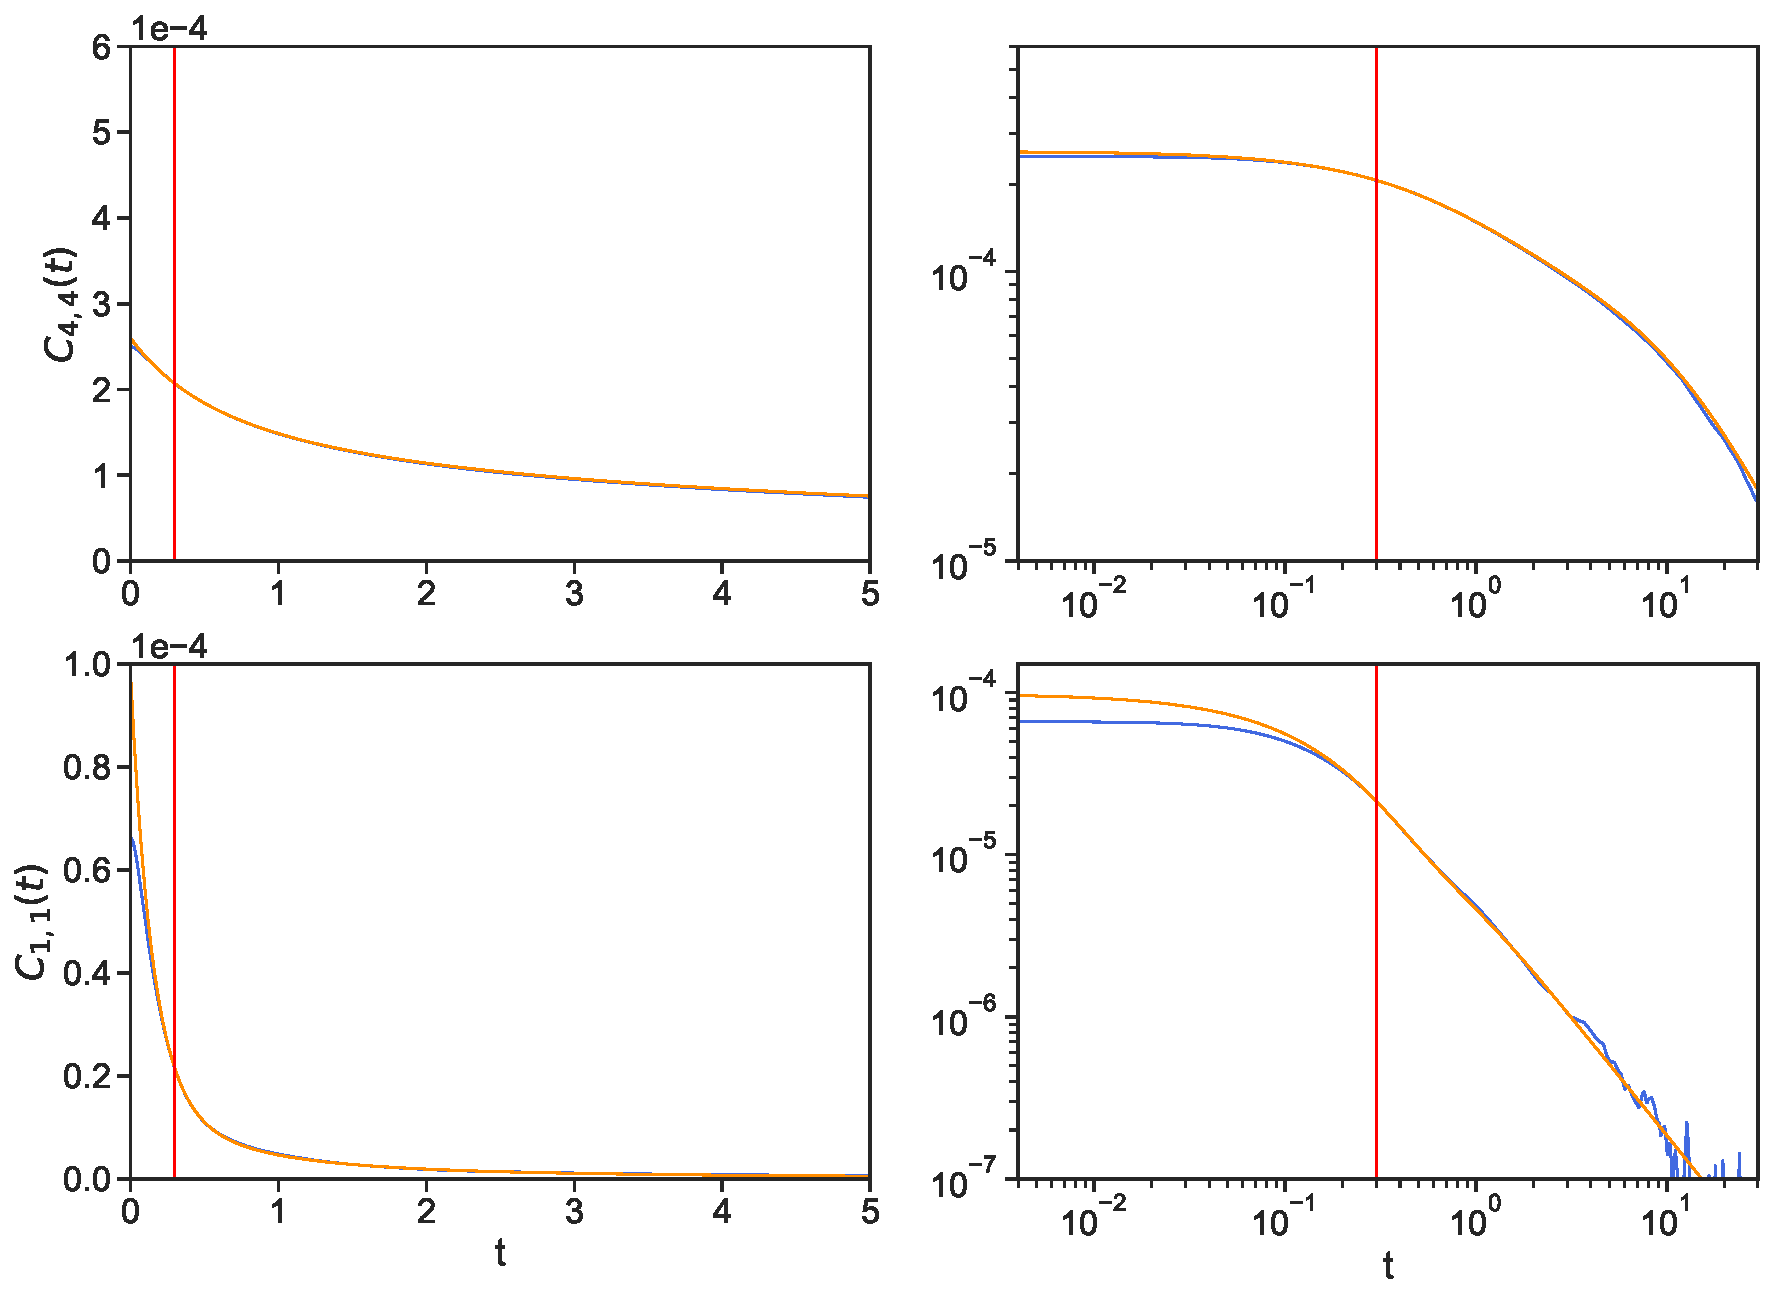
\includegraphics[width=\linewidth]{Predictions-WALLS-17nodes-defense}
%\end{figure}
%\end{frame}
%
%\begin{frame}{Predicted cross-correlations ($\Delta z=2\sigma$)}
%\begin{figure}[h!]
%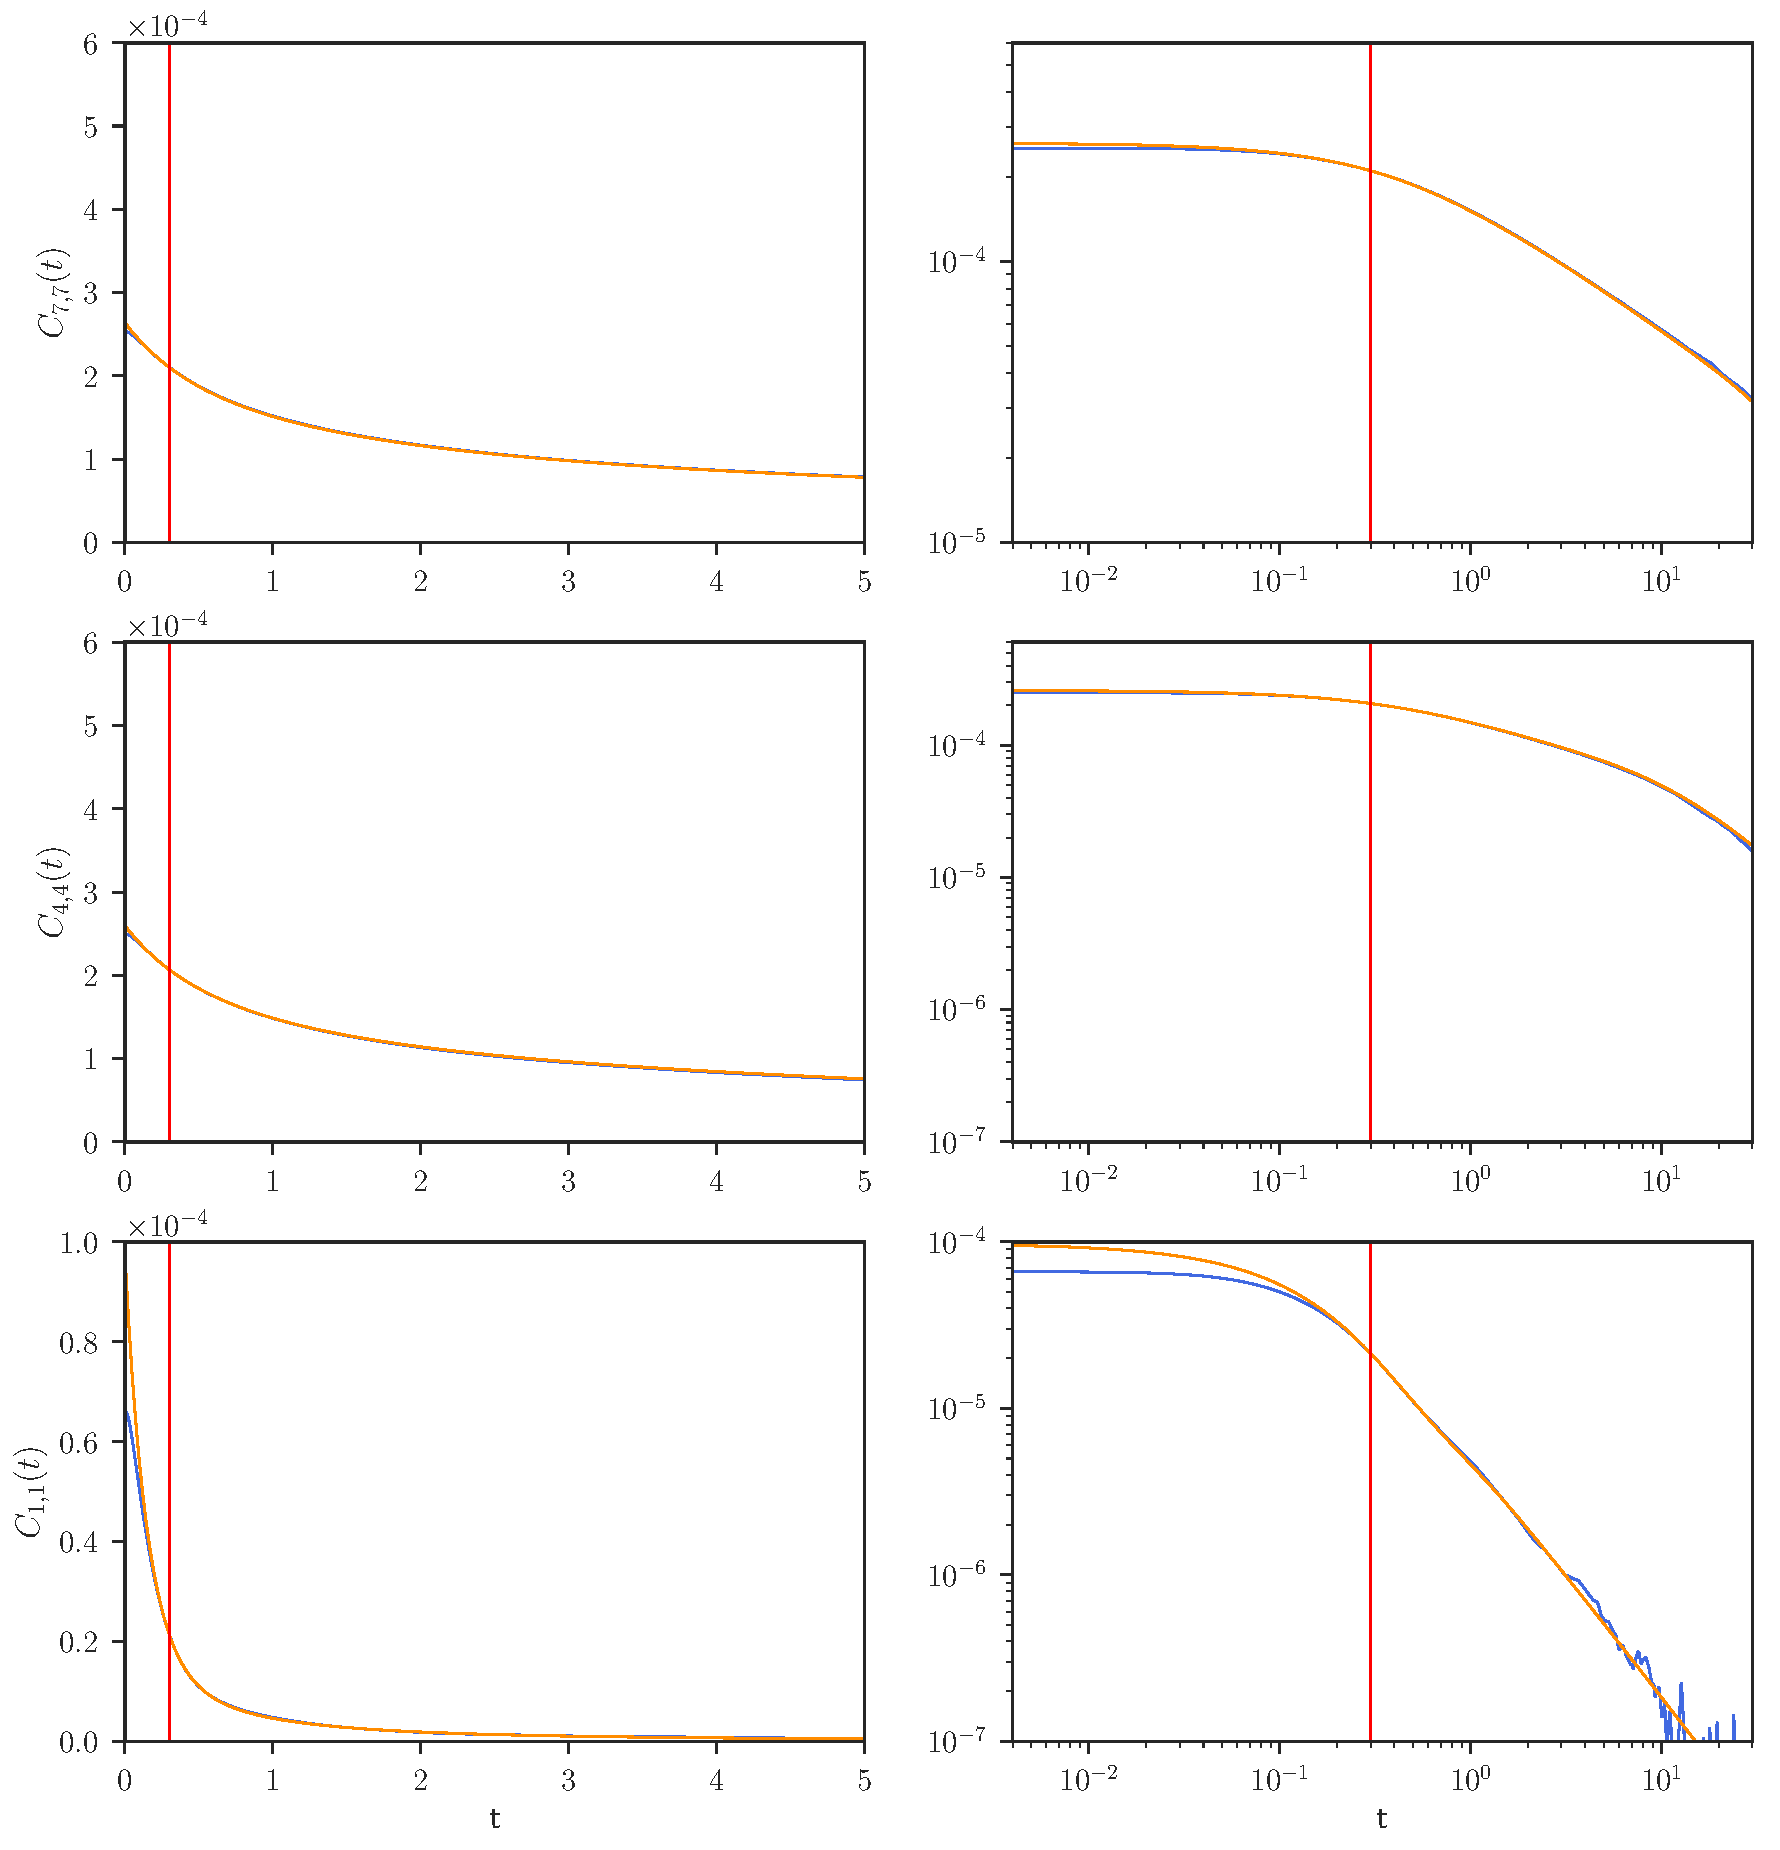
\includegraphics[width=\linewidth]{PredictionsCross-WALLS-17nodes}
%\end{figure}
%\end{frame}
%  
%\begin{frame}{The density}
%\begin{figure}[h!]
%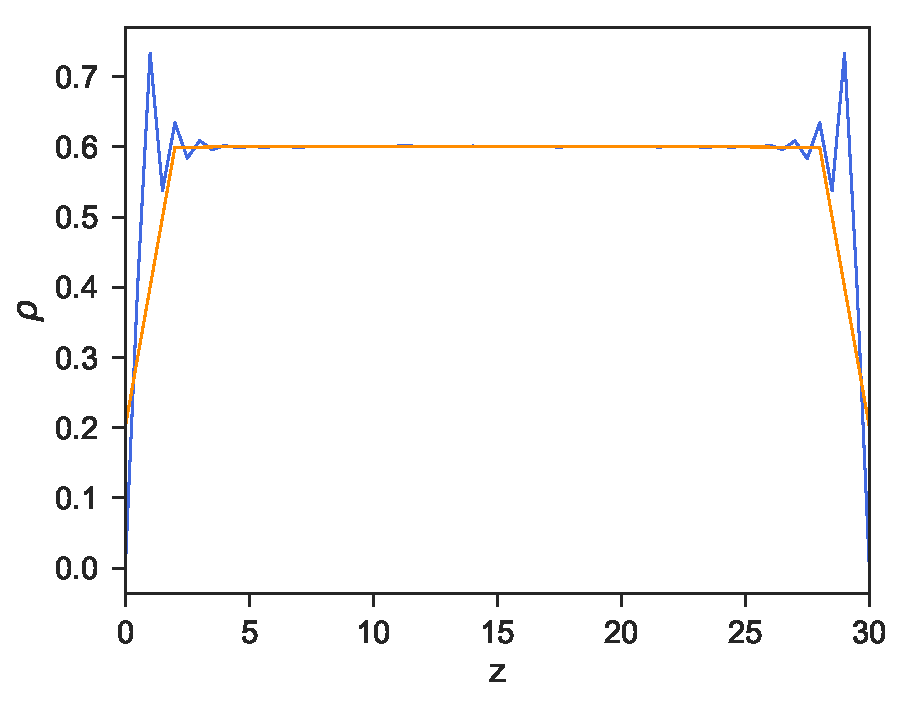
\includegraphics[scale=0.41]{DensityProfile-WALLS}
%\end{figure}
%\end{frame}
%
%\begin{frame}{Summary}
%  \begin{itemize}
%    \item
%    \item
%    \item 
%   \end{itemize}
%\end{frame}
%
%\section{The slip boundary condition}
%\begin{frame}{Overview}
%  \begin{itemize}
%    \item Compute the viscosity and friction kernels that appear in the discrete hydrodynamic theory: $\eta$, $G$, $H$ and $\gamma$. We will use a bin size of $\Delta=2\sigma$ (Markovian behaviour near walls).
%    \item Prediction of $C(t)$ and the average, $g^x(t)$, with these kernels. 
%    \item Derive the Navier slip boundary condition: explicit expression for the slip length.
%    \end{itemize}
%\end{frame}
%
%\begin{frame}{The tine derivative of $C(t)$}
%  \begin{itemize}
%    \item The time derivative of the CG variable $\hat{g}(t)$
%\begin{align}
%  i{\cal L}\hat{g}_\mu(z) &=\hat{F}_\mu(z)-\frac{\hat{\sigma}_\mu(z)-\hat{\sigma}_{\mu-1}(z)}{\Delta z}
%  \nonumber
%\end{align}
%where $\hat{F}_{\mu}=\hat{\bf F}^x_{\mu}$ and $\hat{\sigma}_{\mu}=\hat{\sigma}_{\mu}^{xz}$.
%\item We may express $i{\cal L}\hat{g}$ in a more compact form  
%\begin{align}
%  i{\cal L}\hat{g}&= \hat{F}+ F^T\esc\hat{\sigma}
%  \nonumber
%\end{align}
%\item Time derivative of the correlation matrix 
%  \begin{align}
%    \frac{d}{dt}C(t)=-k_BTM(t)
%    \nonumber
%  \end{align}
%  where $M(t)$ is given by 
%\begin{align}
%M(t)&= \frac{1}{k_BT}\int_0^t dt'\langle i{\cal L}\hat{g}(t')i{\cal L} \hat{g}^T\rangle
%\nonumber
%\end{align}
%  \end{itemize}
%\end{frame}
%
%\begin{frame}{The Green-Kubo running integrals}
%
%  \begin{itemize}
%    \item The matrix $M(t)$ can be expressed as 
%      \begin{align}
%{M}(t)&=F^T\esc{\eta}(t)\esc F+{G}(t)\esc F+F^T\esc{H}(t)+{\gamma}(t),
%\nonumber
%\end{align}
%
%    \item Where the Green-Kubo integrals are
%\begin{align}
%\eta_{\mu\nu}(t)
%&=\frac{1}{k_BT}\int_0^t dt'
%\left\langle \hat{\boldsymbol{\sigma}}^{xz}_{\mu}(t')\hat{\boldsymbol{\sigma}}^{xz}_{\nu}
%\right\rangle
%\nonumber\\
%  G_{\mu\nu}(t)&=\frac{1}{k_BT}\int_0^t dt'
%\left\langle\hat{\bf F}^x_\mu(t')
%\hat{\boldsymbol{\sigma}}^{xz}_\nu
%\right\rangle
%\nonumber\\
%H_{\mu\nu}(t)&=
%\frac{1}{k_BT}\int_0^t dt'
%\left\langle\hat{\boldsymbol{\sigma}}^{xz}_\mu(t')\hat{\bf F}^{x}_\nu\right\rangle
%\nonumber\\
%  \gamma_{\mu\nu}(t)
%&=\frac{1}{k_BT}\int_0^t dt'
%\left\langle 
%\hat{\bf F}^{x}_\mu(t')
%\hat{\bf F}^{x}_\nu\right\rangle
%\nonumber
%\end{align}
%
%\item Therefore, $\frac{d}{dt}C(t)=-k_BTM(t)$ may be expressed as
%\begin{align}
%  \frac{d}{dt}C(t)&=-k_BT\left[{F}^T\esc{\eta}(t)\esc{F}+{G}(t)\esc{F}+{F}^T\esc{H}(t)+{\gamma}(t)\right]
%\nonumber
%\end{align}
%\end{itemize}
%\end{frame}
%
%\begin{frame}{No plateau in the Green-Kubo integrals}
%$\eta_{10,10}(t)$ (middle of the channel), $\gamma_{1,1}$ (blue) and $\gamma_{2,2}$ (orange). 
%\begin{figure}[]
%  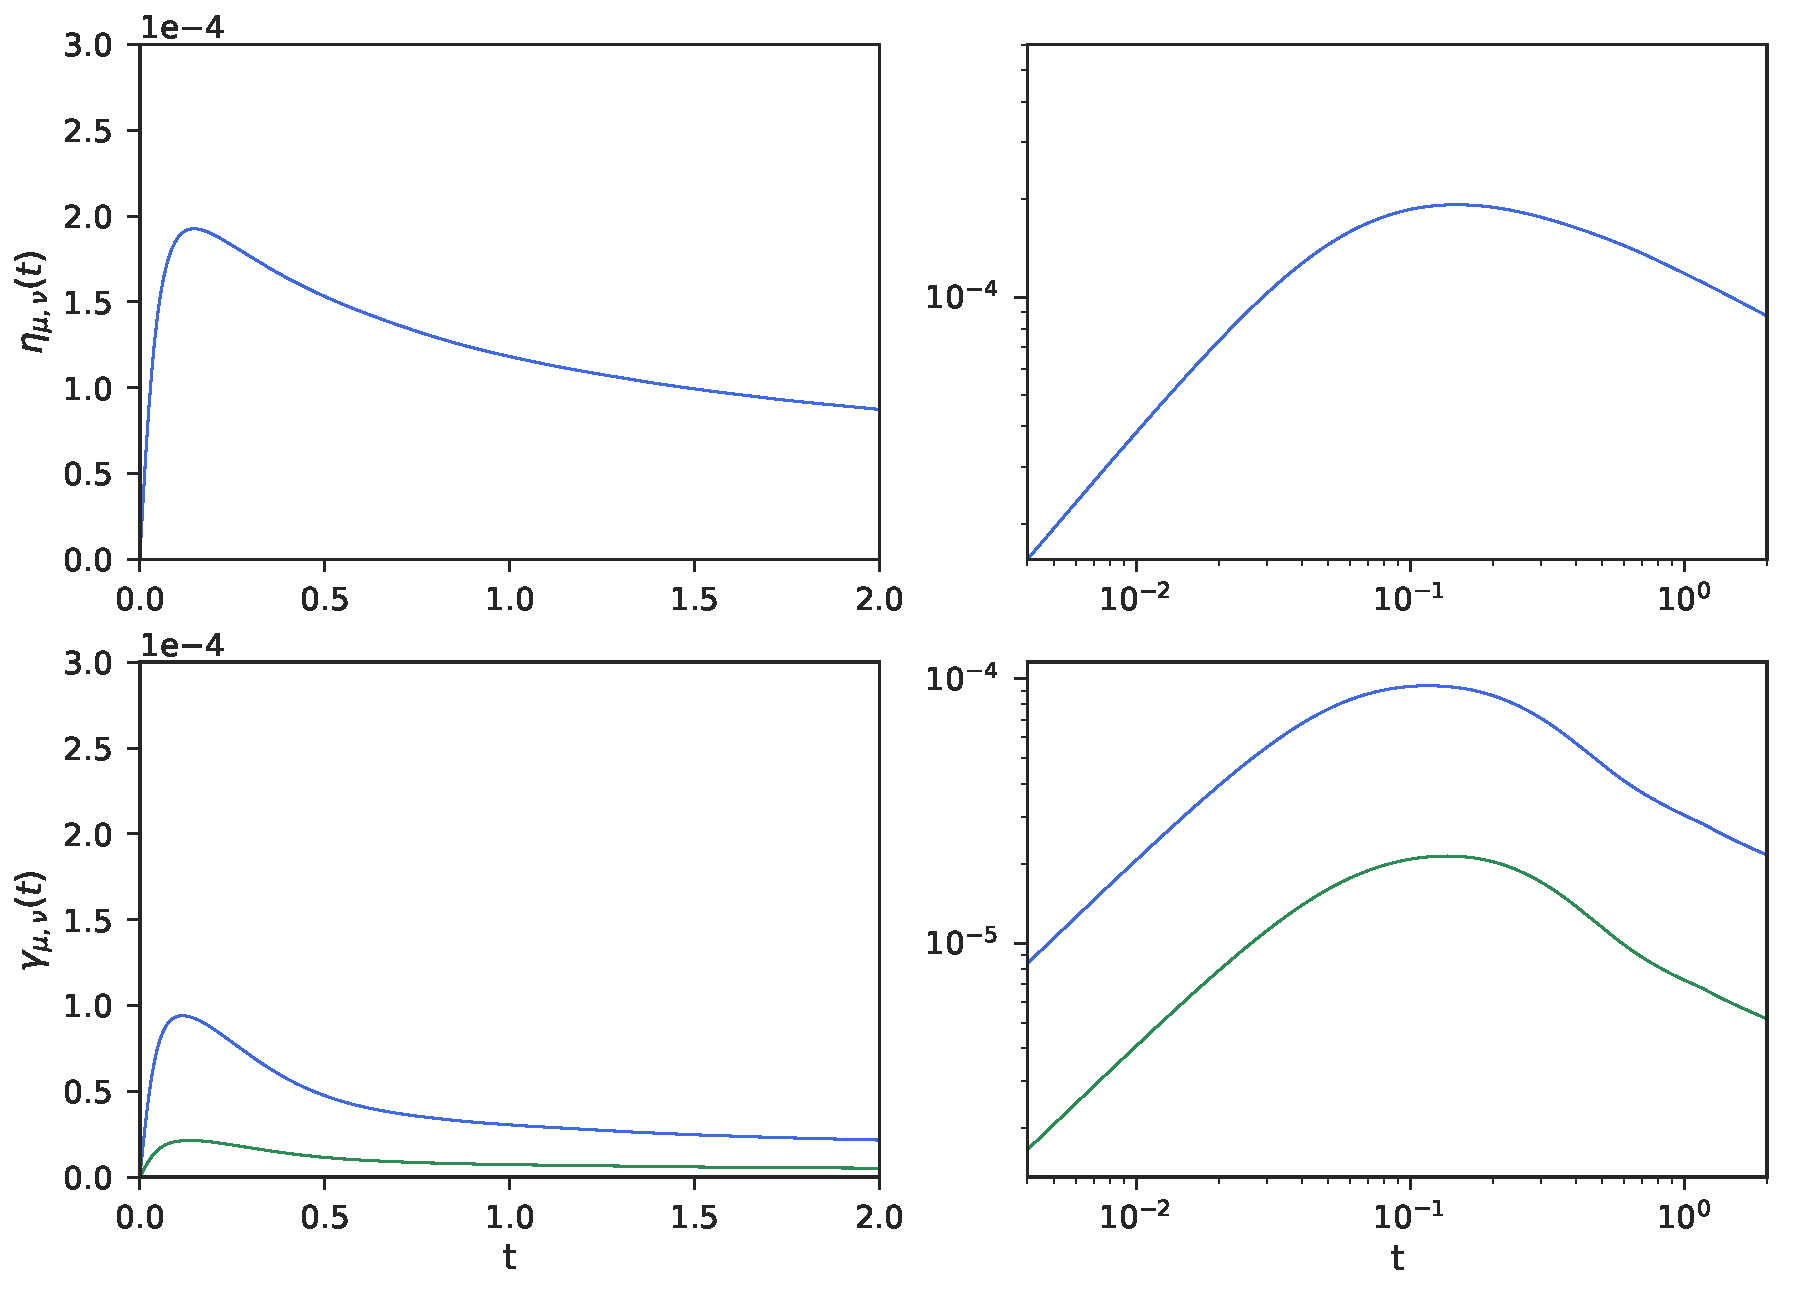
\includegraphics[scale=0.33]{NoPlateau-WALLS-17nodes}
%\end{figure}
%\end{frame}
%
%\begin{frame}{The dynamics of the discrete transverse momentum}
%  \begin{itemize}
%    \item Corrected Green-Kubo formula 
%      \begin{align}
%        M^*=M(\tau)\cdot c^{-1}(\tau)
%        \nonumber
%      \end{align}
%    \item The Markovian dynamics given by Mori theory ($L=0$) 
%      \begin{align}
%        \frac{d}{dt}C(t)=-k_BT^*\cdot C^{-1}(0)C(t)
%        \nonumber
%      \end{align}
%  \item 
%    \begin{align}
%      \frac{d}{dt}C(t)=-k_BT\left[{F}^T\esc{\eta}(t)\esc{F}+{G}(t)\esc{F}+{F}^T\esc{H}(t)+{\gamma}(t)\right]
%      \nonumber
%      \end{align}
%      $\downarrow$
%\begin{align}
%\frac{d}{dt}C(t) =
%-k_BT\left[{F}^T{\eta}(\tau)\esc{F} +{G}(\tau)\esc F+F^T\esc{H}(\tau)+{\gamma}(\tau)\right]& \nonumber \\
%\times C^{-1}(\tau) \esc C(t)&
%\nonumber
%\end{align}
%
%\end{itemize}
%\end{frame}
%
%\begin{frame}{The equation for the average of the discrete momentum field}
%  \begin{itemize}
%    \item Algo
%\begin{align}
%   \frac{d}{dt}g(t)= -k_BT \left[{F}^T{\eta}(\tau)\esc{F}
%+{G}(\tau)\esc{F}
%+F^T\esc{H}(\tau)+{\gamma}(\tau)\right]& \nonumber \\
%\times C^{-1}(\tau)\esc  g(t)& 
%\nonumber
%\end{align}
%\item In terms of the velocity 
%\begin{align}
%  \frac{d}{dt}g(t)&= -\left[{F}^T{\eta}(\tau)\esc{F}
%+{G}(\tau)\esc{F}
%+F^T\esc{H}(\tau)+{\gamma}(\tau)\right]&& \nonumber \\
%\times {\cal V} \esc c^{-1}(\tau)\esc v(t)&& \nonumber \\
% &= - {\cal V}\esc M^*\esc v(t) 
%\nonumber
%\end{align}
%\item It is equivalent to 
%\begin{align}
%   \frac{d}{dt}g(t)&=  - {\cal V}\esc M(\tau)\esc \overline{v}(t)
%\nonumber
%\end{align}
%\item The scaled velocity field $\overline{v}(t)=c^{-1}(\tau)\esc  v$.
%\end{itemize}
%\end{frame}
%
%\begin{frame}{The dynamics with the scaled velocity field}
%  \begin{itemize}
%    \item The  components $\overline{\bf  v}^x_\mu$  of
%$\overline{v}$ are
%\begin{align}
%  \overline{\bf v}^x_\mu&=\sum_{\nu}\overline{\rho}_{\mu\nu}^{-1}{\bf g}^x_\nu
%\nonumber
%\end{align}
%\item The rescaled mass density is 
%\begin{align}
%  \overline{\rho}_{\mu\nu}&=\frac{C_{\mu\nu}(\tau)}{k_BT}  {\cal V}_\mu
%  \nonumber
%\end{align}
%\item The explicit form of the evolution of the average of the discrete momentum field 
%\begin{align}
%  \frac{d}{dt}{\bf g}^x_\mu(t)=&
%-\sum_{\nu} {\cal V}_\nu \frac{\left[\eta_{\mu\nu}-\eta_{\mu-1\nu}-\eta_{\mu\nu-1}+\eta_{\mu-1\nu-1}\right]}{\Delta z^2}\overline{\bf v}^x_\nu
%\nonumber \\
%&+\sum_{\nu} {\cal V}_\nu\frac{\left[G_{\mu\nu}-G_{\mu\nu-1}\right]}{\Delta z}\overline{\bf v}^x_\nu
%\nonumber\\
%&+\sum_{\nu} {\cal V}_\nu\frac{\left[H_{\mu\nu}-H_{\mu-1\nu}\right]}{\Delta z}
%\overline{\bf v}^x_\nu
%-\sum_{\nu} {\cal V}_\nu\gamma_{\mu\nu}\overline{\bf v}^x_\nu,
%\nonumber
%\end{align}
%    \end{itemize}
%\end{frame}
%
%\begin{frame}{Evolution of the flow in NEMD simulations}
%  \begin{itemize}
%  \item Plug flow simulation.
%  \item We add to the thermal velocity of each fluid atom the same velocity ${\bf V}=(v_0,0,0)$
%    \begin{itemize}
%      \item Nonequilibrium plug flow parallel to the wall. 
%      \item Increase the temperature of the system. 
%      \end{itemize}
%    \item We rescale the resulting velocities to remain at the same temperature. 
%    \item Repeat the procedure with different initial configurations. 
%  \end{itemize}
%\end{frame}
%
%\begin{frame}{Evolution of the flow in NEMD simulations - Predictions}
%  \begin{itemize}
%    \item Mori theory of the evolution of the average $\hat{{\bf g}}^x(t)$ 
%      \begin{align}
%        \frac{d}{dt}g(t) = \Lambda^*\esc g(t)
%        \nonumber
%      \end{align}
%      where the relaxation matrix is $\Lambda^*=k_BTM^*\esc C^{-1}(0)$
%    \item Matrix exponential solution
%\begin{align}
%  g(t)=\exp\{-\Lambda^* (t-\tau)\}\esc g(\tau)
%\nonumber
%\end{align}
%    \end{itemize}
%\begin{figure}[!h]
%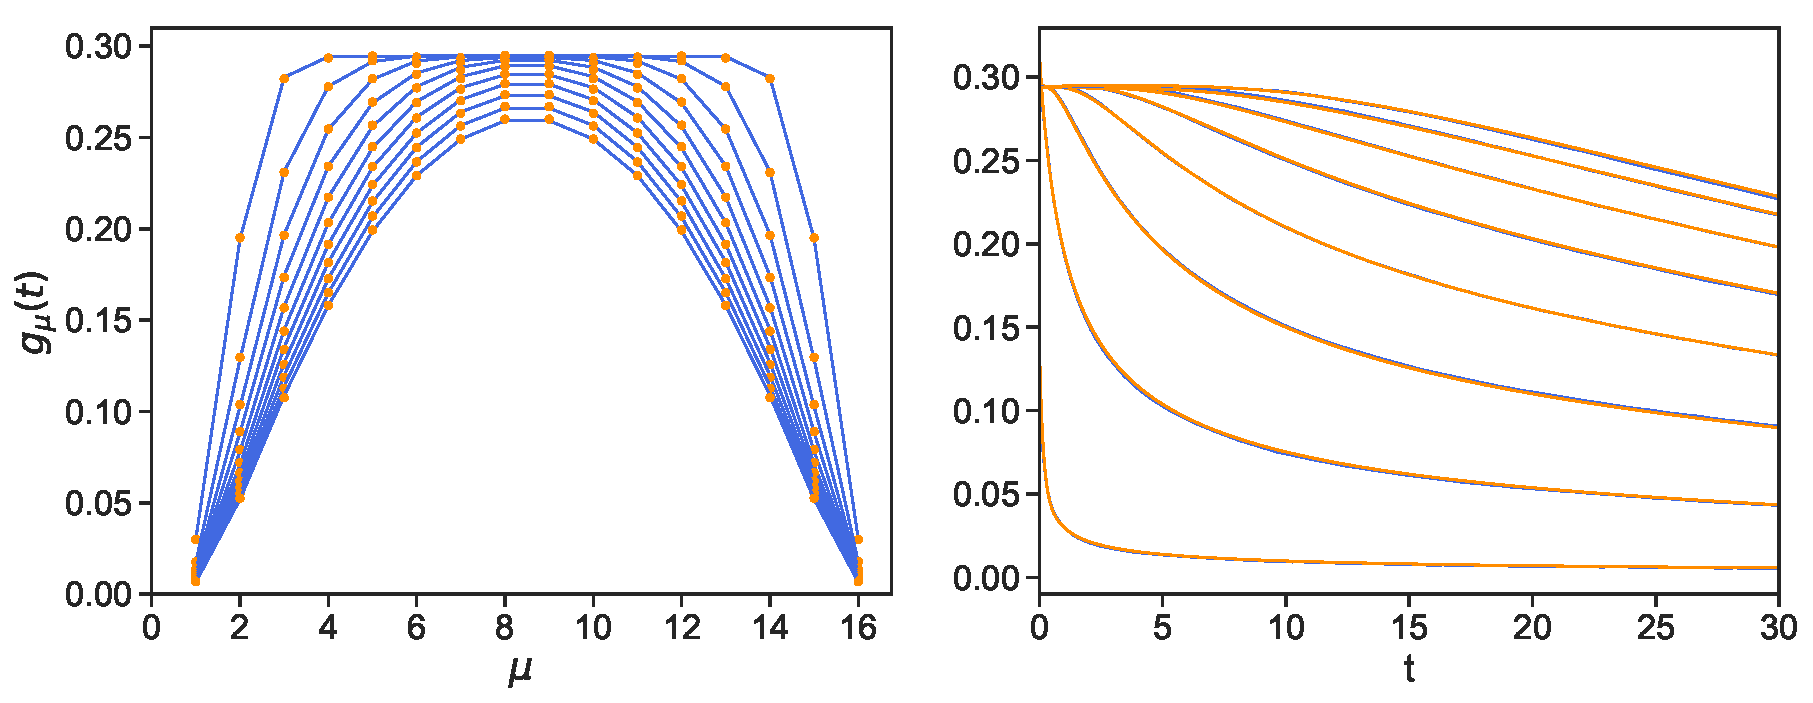
\includegraphics[width=\linewidth]{gxtPredictions-17nodes-WALLS-defense}
%\end{figure}
%\end{frame}
%
%\begin{frame}{The boundary slab}
%  \begin{itemize}
%    \item Boundary slab of fluid which is made of $B$ bins.
%    \item The momentum ${\bf P}_B^x$ of this slab
%\begin{align}
%{\bf P}_B^x&\equiv  \sum^{B}_{\mu=0}{\cal    V}_\mu    \hat{\bf    g}^x_\mu=\sum_i^N{\bf    p}_iU_B(z_i)
%  \nonumber
%\end{align}
%\item The function $U_B(z)$ counts the number of particles near the wall
%\begin{align}
%  U_B(z)=\sum_\mu^{B}{\cal    V}_{\mu}\delta_\mu(z)  
%  \nonumber
%\end{align}
%\begin{figure}[]
%  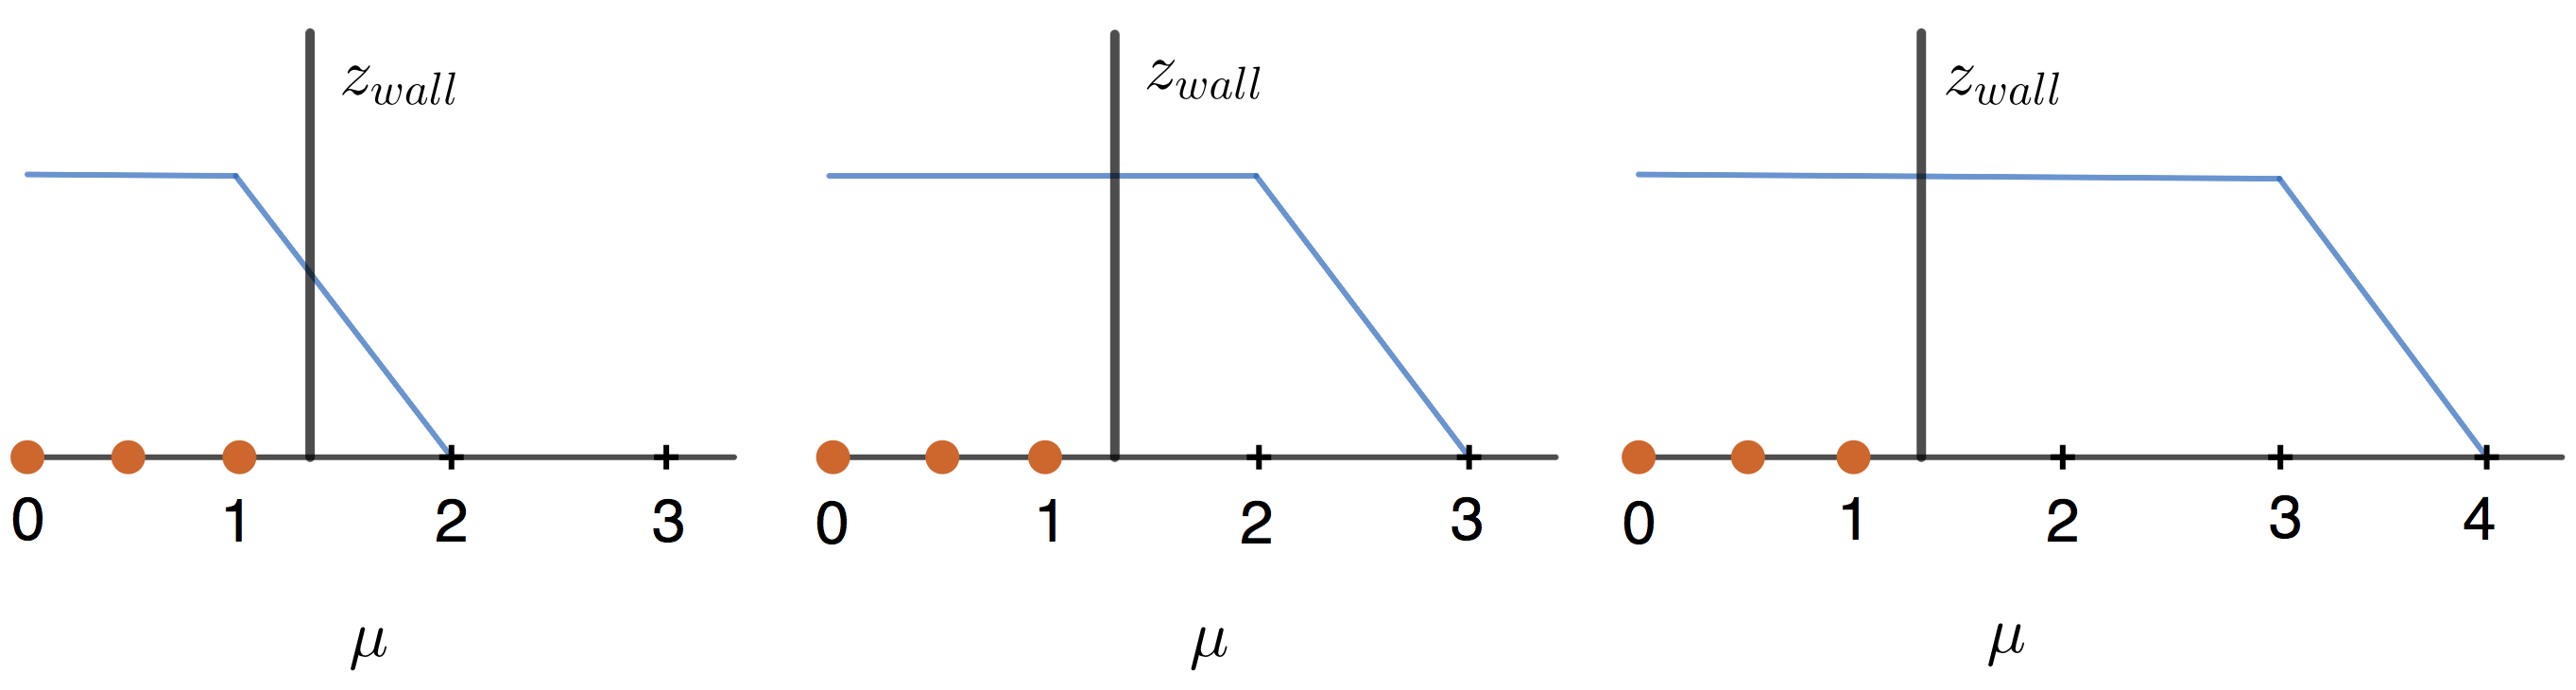
\includegraphics[width=\linewidth]{SchemeBSlab-defense}
%\end{figure}
%    \end{itemize}
%\end{frame}
%
%\begin{frame}{The mechanical balance}
%  \begin{itemize}
%    \item The total force on the slab
%\begin{align}
%{\bf F}^x_B(t)&=\frac{d}{dt} \sum^{B}_{\mu=0}{\cal V}_\mu  {\bf g}^x_\mu(t)
%\nonumber
%\end{align}
%\item In terms of the local transport coeffients 
%\begin{align}
%\frac{1}{S}{\bf F}^x_B=  \sum_{\nu} {\cal V}_\nu 
%\left[\eta_{B\nu}-G_\nu \right]\frac{\overline{\bf v}^x_{\nu+1}-\overline{\bf v}^x_{\nu}}{\Delta z}
%-\sum_{\nu=0} {\cal V}_\nu\left[\gamma_{\nu}-H_{B\nu}\right]\overline{\bf v}^x_\nu,
%\nonumber
%\end{align}
%where the following local transport coefficients have been defined
%\begin{align}
%  G_\nu\equiv \frac{1}{S} \sum^{B}_{\mu=1}{\cal V}_\mu G_{\mu\nu}, &&
%\gamma_{\nu}\equiv  \frac{1}{S}\sum^{B}_{\mu=1}{\cal V}_\mu \gamma_{\mu\nu}
%\nonumber
%\end{align}
%    \end{itemize}
%\end{frame}
%
%\begin{frame}{Transport coefficients}
%  \begin{figure}[]
%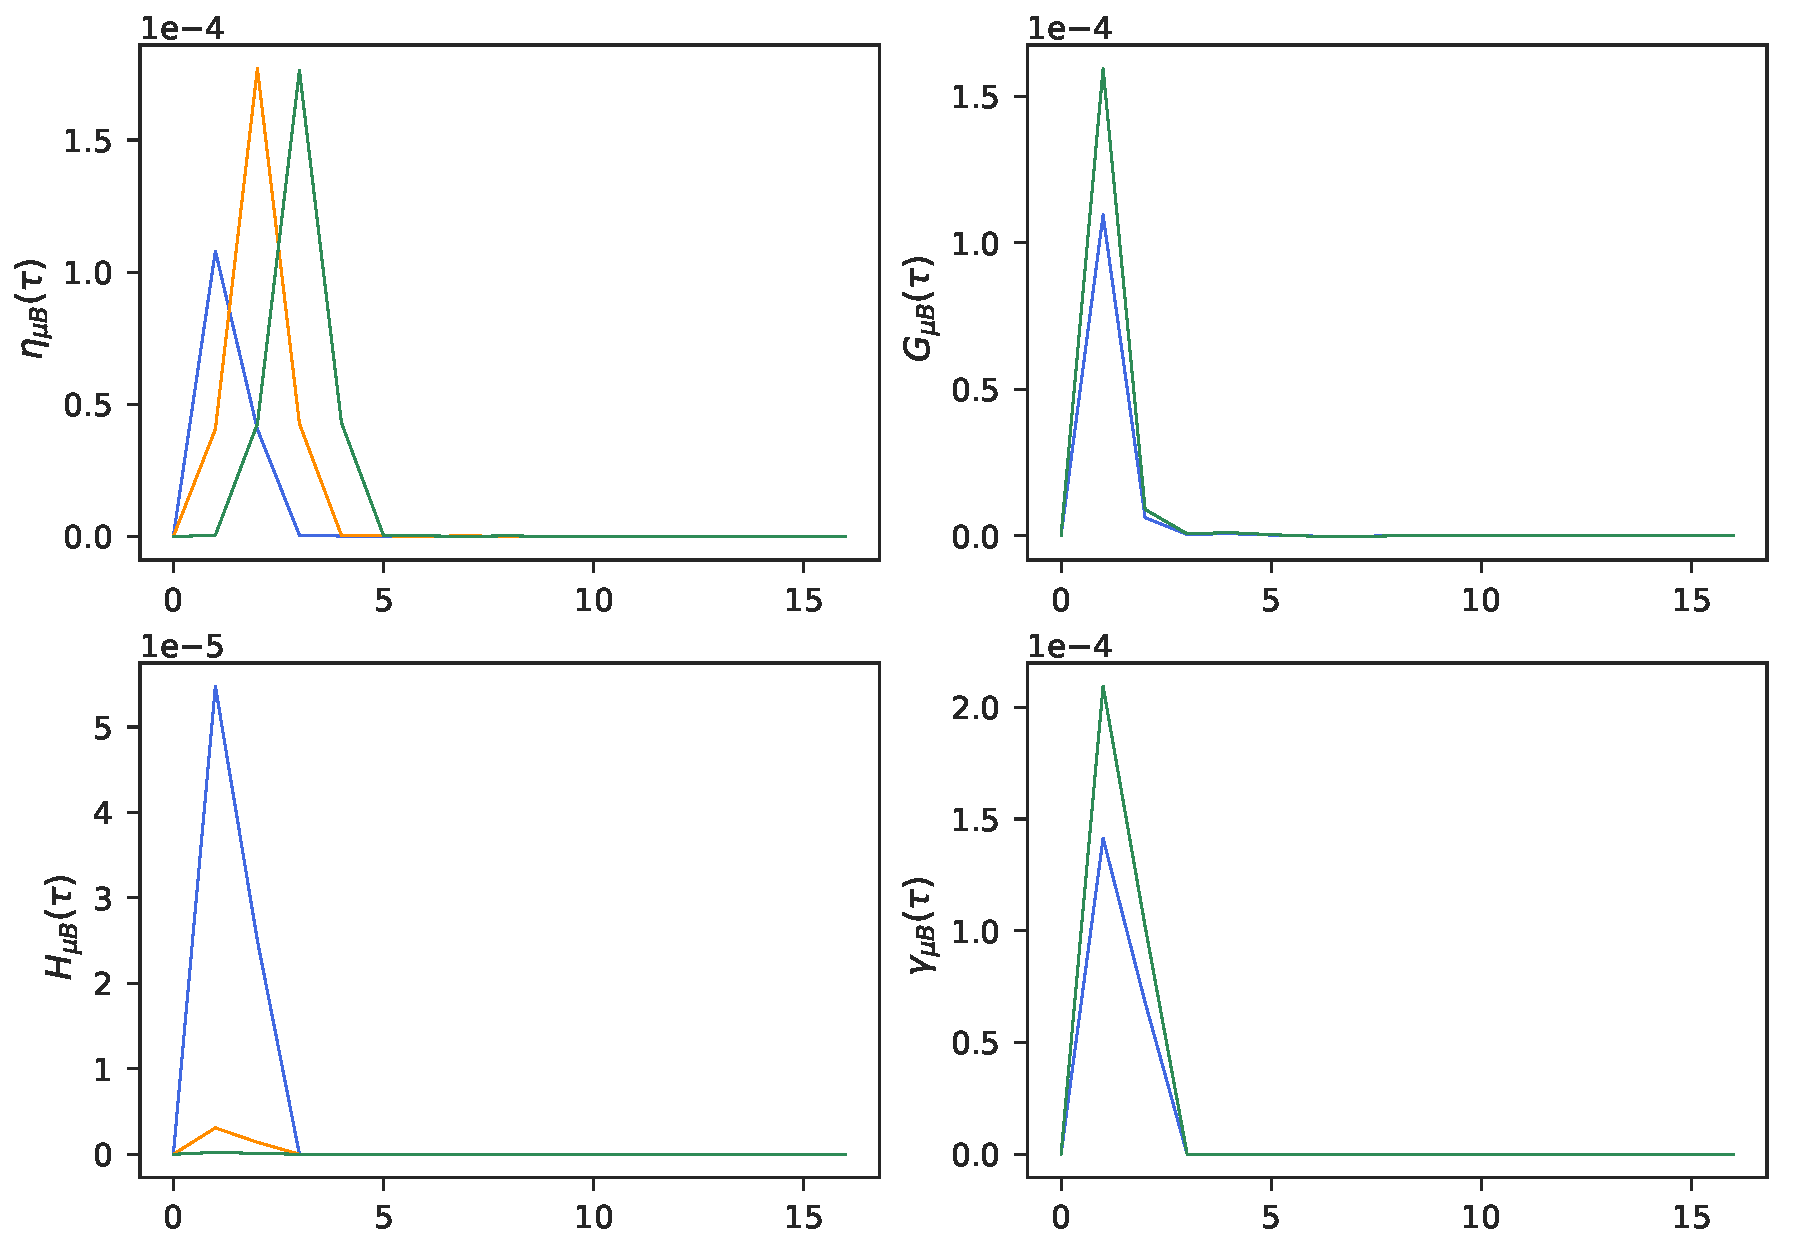
\includegraphics[width=\linewidth]{transportMatrices-17nodes-WALLS}
%\end{figure}
%\end{frame}
%
%\begin{frame}{The boundary condition}
%  \begin{itemize}
%    \item Assume that the velocity inside the boundary slab is linear
%\begin{align}
%\overline{\bf v}^x_{\mu}&=  \overline{\bf v}^x_{\rm wall}+\dot{\overline{\gamma}}_{\rm wall}(\mu\Delta z-z_{\rm wall})
%\nonumber
%\end{align}
%\item With $B=2$ the force on the boundary is due to the velocity of nodes $\mu=1,2,3,4$
%\begin{align}
%\frac{1}{S}{\bf F}^x_B=  \sum_{\nu=1}^{B+1} {\cal V}_\nu 
%\left[\eta_{B\nu}-G_\nu \right]\frac{\overline{\bf v}^x_{\nu+1}-\overline{\bf v}^x_{\nu}}{\Delta z}
%-\sum_{\nu=1}^{B} {\cal V}_\nu\left[\gamma_{\nu}-H_{B\nu}\right]\overline{\bf v}^x_\nu
%\nonumber
%\end{align}
%\item Therefore
%\begin{align}
%\frac{1}{S}{\bf F}^x_B&=\eta'\dot{\overline{\gamma}}_{\rm wall}
%-\gamma'\overline{\bf v}^x_{\rm wall}
%\nonumber
%\end{align}
%\item  We have introduced the transport coefficients
%\begin{align}
%  \eta'=   \eta - G, &&
%\gamma'=  \gamma-H
%\nonumber
%\end{align}
%    \end{itemize}
%\end{frame}
%
%\begin{frame}{Check mechanical balance for B=2}
%\begin{align}
%  {\color{green} \frac{1}{S}{\bf F}^x_B}={\color{blue}
%-\gamma'\overline{\bf v}^x_{\rm wall}
%\sum_{\nu=1}^{B+1} {\cal V}_\nu 
%\left[\eta_{B\nu}-G_\nu \right]\frac{\overline{\bf v}^x_{\nu+1}-\overline{\bf v}^x_{\nu}}{\Delta z}
%-\sum_{\nu=1}^{B} {\cal V}_\nu\left[\gamma_{\nu}-H_{B\nu}\right]\overline{\bf v}^x_\nu
%}
%\nonumber
%\end{align}
%\begin{figure}[]
%  \centering
%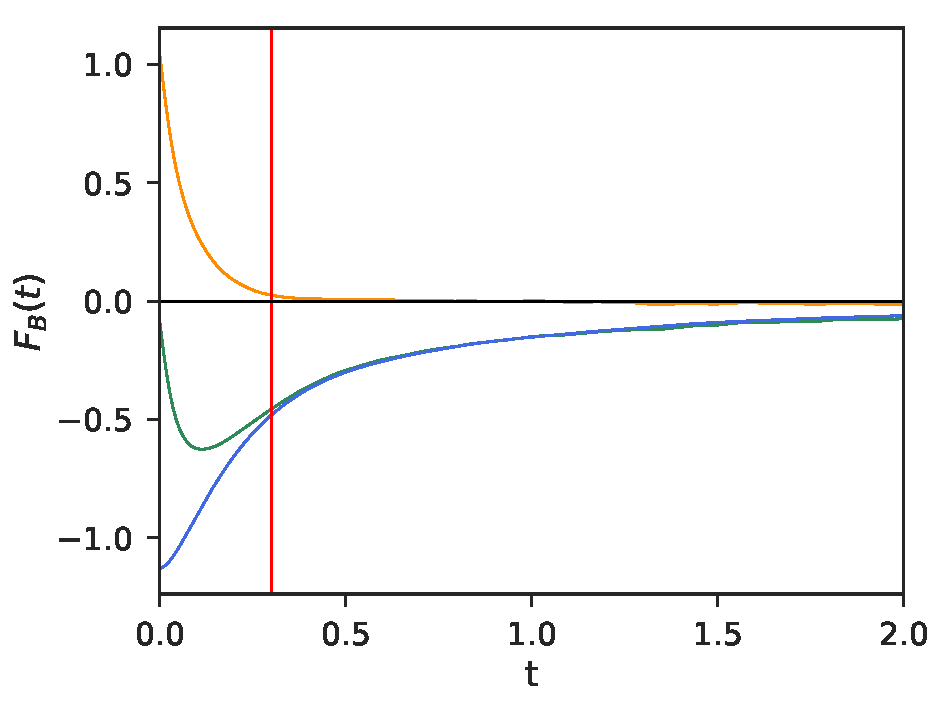
\includegraphics[scale=0.5]{checkMecBalance-17nodes-WALLS}
%\end{figure}
%\end{frame}
%
%\begin{frame}{The slip length}
%  \begin{itemize}
%    \item
%When the force on the boundary slab vanishes,
%$ {\bf F}^x_B(t)\simeq 0$, we obtain the Navier
%slip boundary condition
%\begin{align}
%\overline{\bf v}^x_{\rm wall}&=\delta\dot{\overline{\gamma}}_{\rm wall}
%\nonumber
%\end{align}
%\item with the slip length given by
%\begin{align}
%  \delta =\frac{\eta'}{\gamma'}
%\nonumber
%\end{align}
%\end{itemize}
%\end{frame}
%
%\begin{frame}{}
%  \Note{O figura de la slip lenght o derivación microscópica de la slip lenght}
%\end{frame}
%\end{document}
